\chapter[Desenvolvimento]{Desenvolvimento}
\label{cap:desenvolvimento}

Este capítulo tem como objetivo de relatar a implementação da proposta descrita no Capítulo \ref{cap:metodologia} e as atualizações que foram realizadas durante o desenvolvimento.

\section[Modificações na Arquitetura]{Modificações na Arquitetura}
\label{sec:modificacoes-arquitetura}

Foram efetuadas mudanças na arquitetura do \textit{frontend} descrita na Subseção \ref{arquitetura-frontend}. Durante o desenvolvimento da US01, os autores notaram uma vulnerabilidade na forma que as requisições ao \textit{backend} estavam sendo realizadas. Ao serem chamadas diretamente pela página, o usuário conseguia ver detalhes sensíveis das requisições no console do navegador: sua URL (\textit{Uniform Resource Locator}) completa, revelando o endereço do \textit{backend}, o corpo da requisição e também sua resposta. Isso pode ser observado nas Figuras \ref{fig:endpointExpostoURL}, \ref{fig:endpointExpostoCorpo} e  \ref{fig:endpointExpostoResposta}.

\clearpage

\begin{landscape}
    \setlength{\oddsidemargin}{\evensidemargin}
    \numeracaoPaisagem
    \begin{figure}[H]
        \centering
        \caption{Exposição da URL completa da requisição ao usuário.} 
        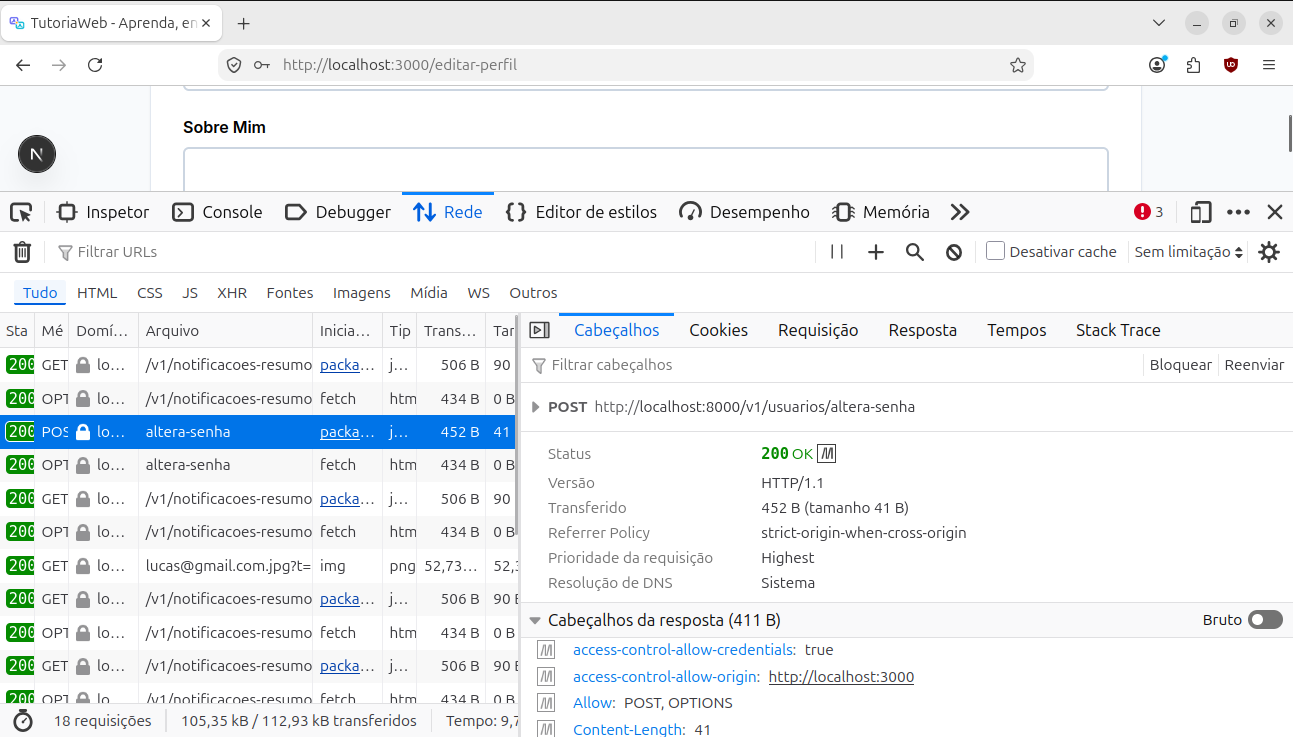
\includegraphics[width=1.9\textwidth, height=0.90\textheight, keepaspectratio]{figuras/endpointExpostoURL.png}
    
    
        Fonte: Autoria própria.
        
        \vspace{0.2cm}
            
        \label{fig:endpointExpostoURL}
    \end{figure}
\end{landscape}

\clearpage

\begin{landscape}
    \setlength{\oddsidemargin}{\evensidemargin}
    \numeracaoPaisagem
    \begin{figure}[H]
        \centering
        \caption{Exposição do corpo da requisição ao usuário.} 
        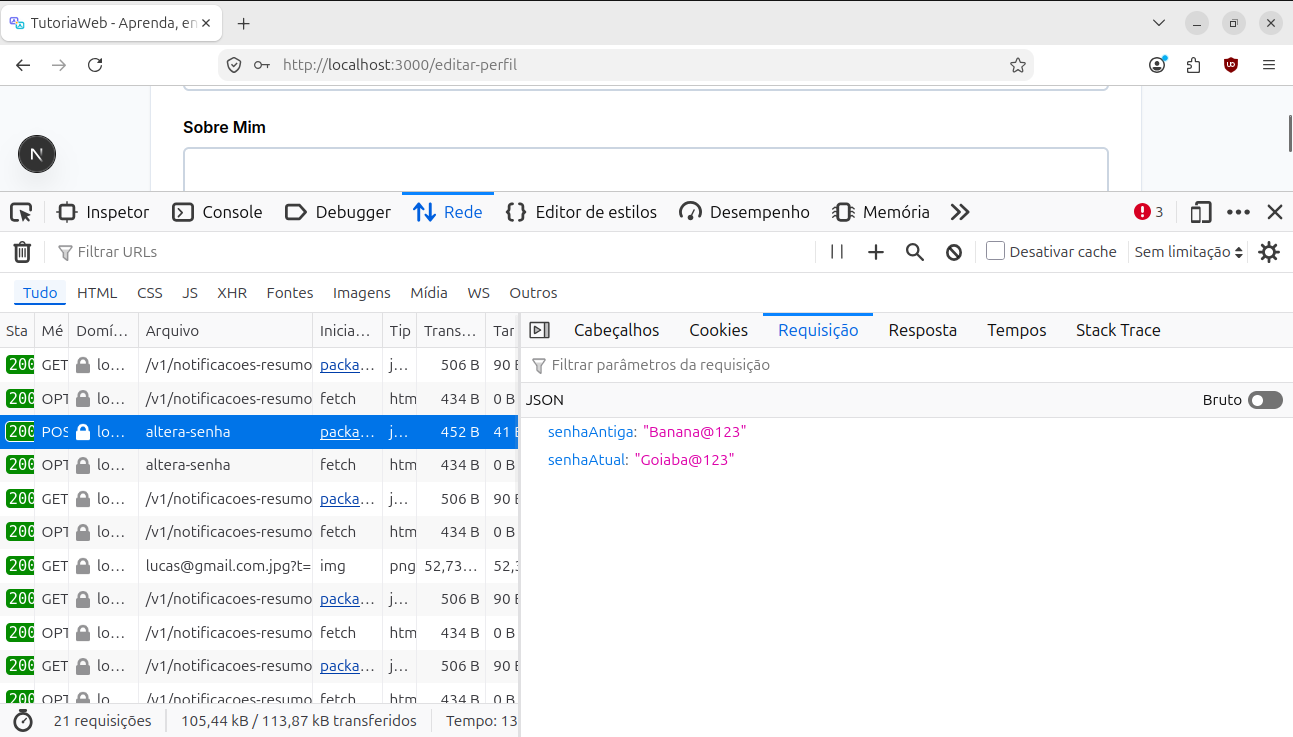
\includegraphics[width=1.9\textwidth, height=0.90\textheight, keepaspectratio]{figuras/endpointExpostoCorpo.png}
    
    
        Fonte: Autoria própria.
        
        \vspace{0.2cm}
            
        \label{fig:endpointExpostoCorpo}
    \end{figure}
\end{landscape}


\clearpage

\begin{landscape}
    \setlength{\oddsidemargin}{\evensidemargin}
    \numeracaoPaisagem
    \begin{figure}[H]
        \centering
        \caption{Exposição da resposta da requisição ao usuário.} 
        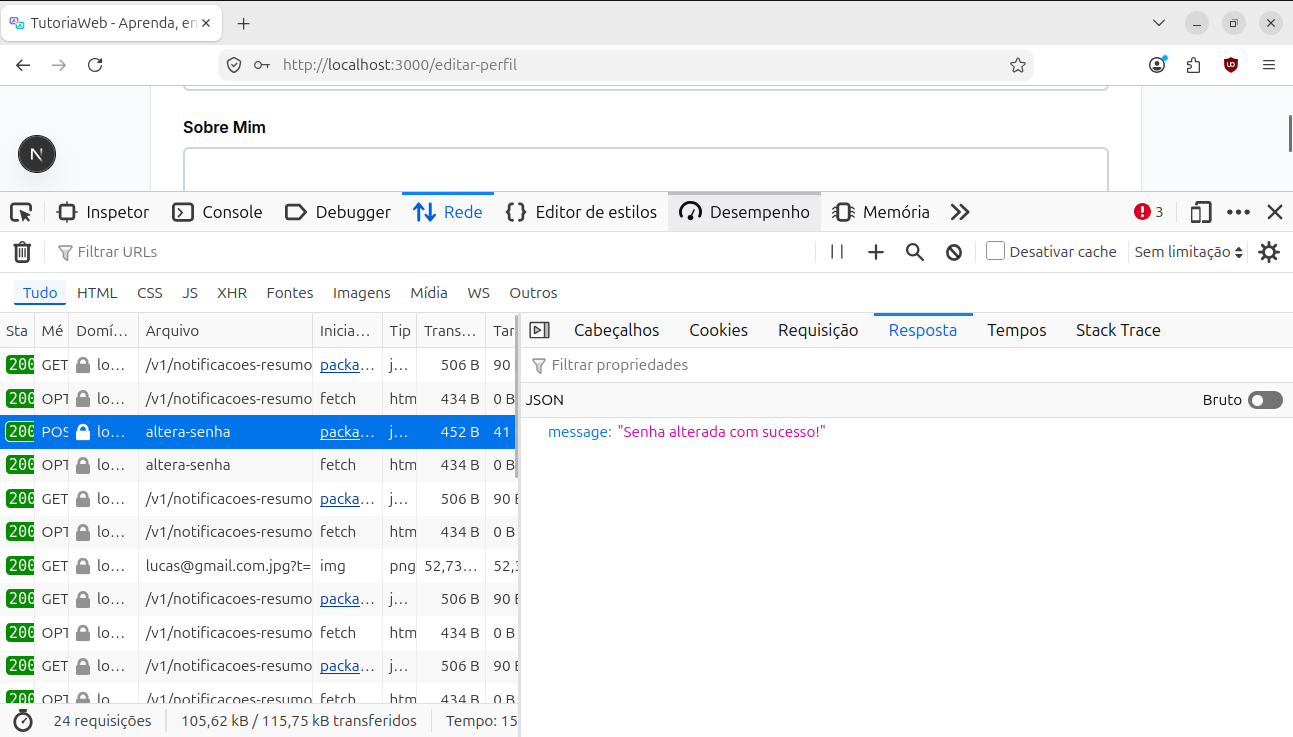
\includegraphics[width=1.9\textwidth, height=0.90\textheight, keepaspectratio]{figuras/endpointExpostoResposta.png}
    
    
        Fonte: Autoria própria.
        
        \vspace{0.2cm}
            
        \label{fig:endpointExpostoResposta}
    \end{figure}
\end{landscape}

Essa vulnerabilidade representava um sério risco à segurança da aplicação, uma vez que usuários maliciosos poderiam usar essas informações para prejudicar o \textit{backend} da aplicação, realizando sucessivas requisições \textit{POST} para sobrecarregar o banco de dados ou requisições \textit{PUT} e \textit{PATCH} para alterar registros do banco.

A solução dos autores foi utilizar as \textit{Server Actions} do Next.js. Server Actions são requisições assíncronas que são executadas pelo servidor \cite{nextjs2026}. Essa característica faz com que os \textit{logs} e processamento da requisição sejam realizados inteiramente pelo servidor, podendo retornando apenas o resultado para o cliente (no caso, a página da aplicação).

A arquitetura foi modificada para incluir \textit{Server Actions} intermediárias entre a página e o backend. A página não executa uma requisição diretamente para o \textit{backend}, e sim uma \textit{Server Action} que realiza a requisição e retorna seus resultados para a página. Essa mudança resolveu a vulnerabilidade, visto que as informações sensíveis são ocultadas do console, sendo exibido apenas a própria rota da página atual, os dados enviados (mas sem revelar a estrutura do corpo da requisição) e o código de resultado da \textit{Server Action}. Isso pode ser observado na Figuras \ref{fig:ocultacaoURL}, \ref{fig:ocultacaoCorpo} e \ref{fig:ocultaçãoResponse}.

\clearpage

\begin{landscape}
    \setlength{\oddsidemargin}{\evensidemargin}
    \numeracaoPaisagem
    \begin{figure}[H]
        \centering
        \caption{Ocultação da URL da requisição ao usuário.} 
        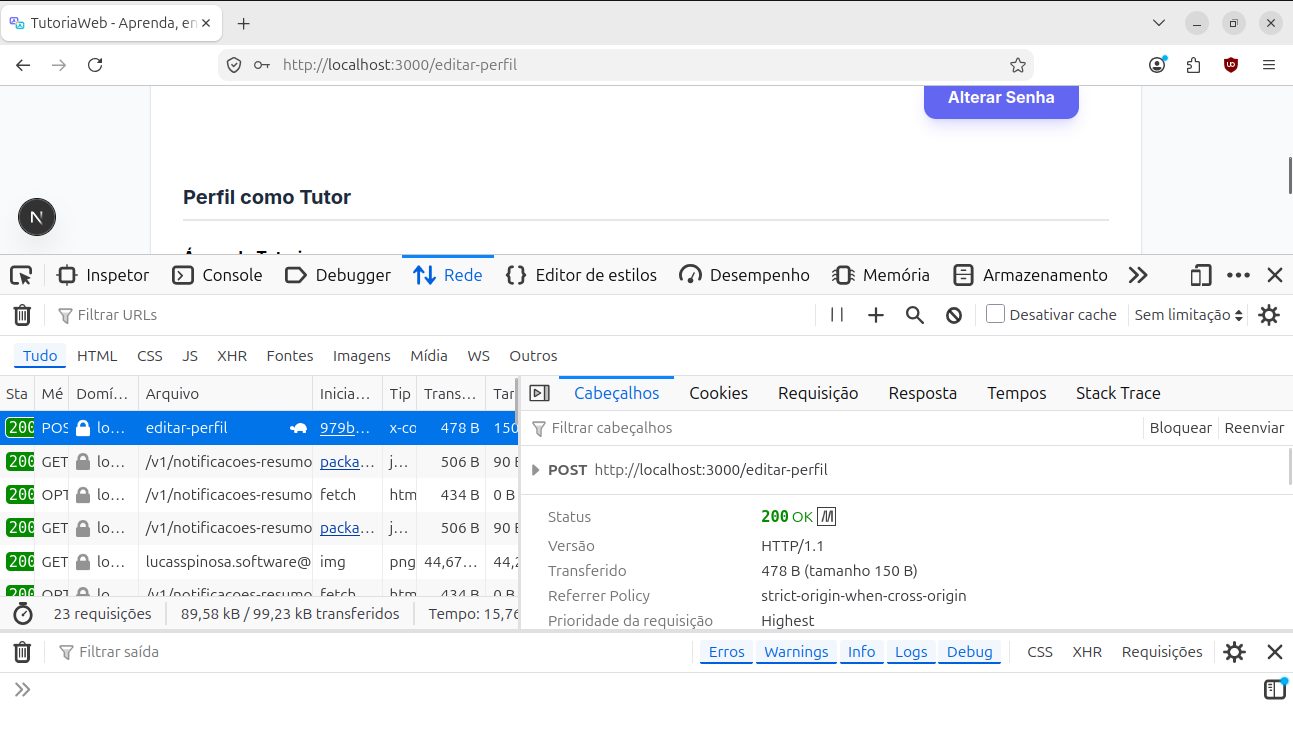
\includegraphics[width=1.9\textwidth, height=0.90\textheight, keepaspectratio]{figuras/ocultacaoURL.png}
    
        Fonte: Autoria própria.
        
        \vspace{0.2cm}
            
        \label{fig:ocultacaoURL}
    \end{figure}
\end{landscape}

\clearpage

\begin{landscape}
    \setlength{\oddsidemargin}{\evensidemargin}
    \numeracaoPaisagem
    \begin{figure}[H]
        \centering
        \caption{Ocultação do corpo da requisição ao usuário.} 
        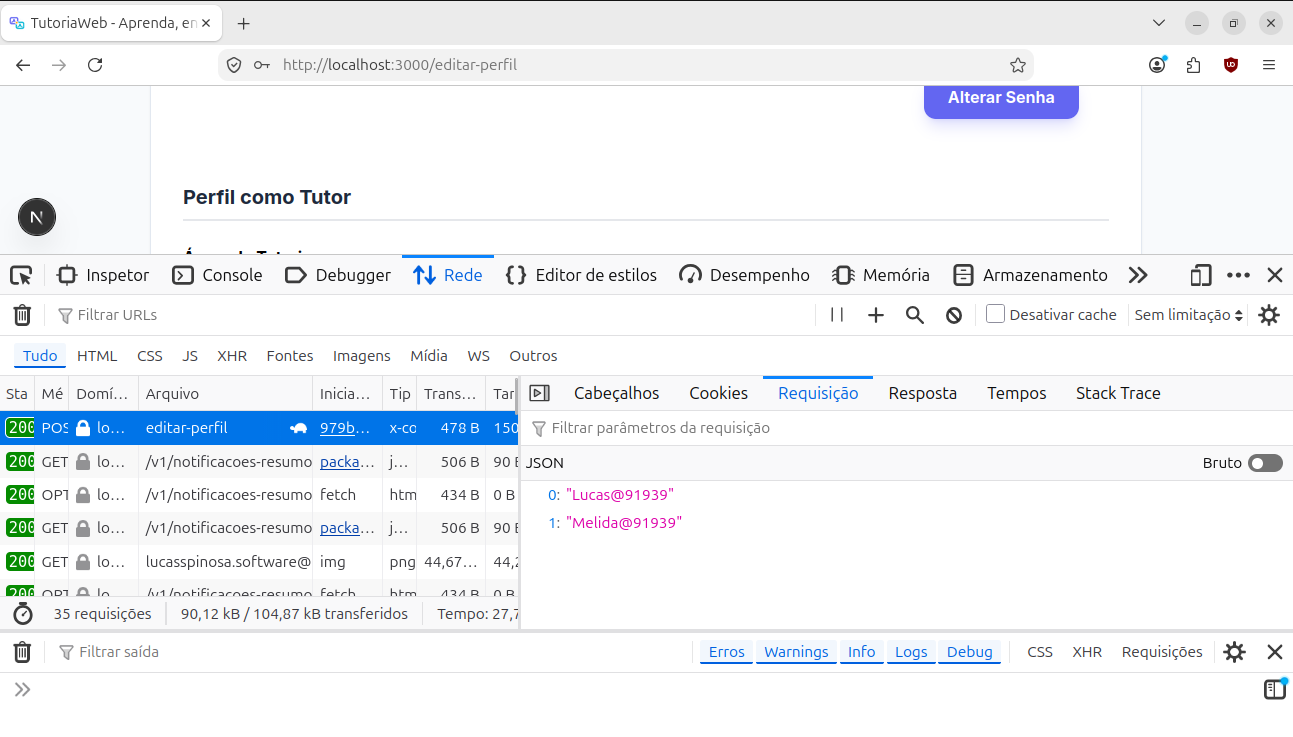
\includegraphics[width=1.9\textwidth, height=0.90\textheight, keepaspectratio]{figuras/ocultacaoCorpo.png}
    
    
        Fonte: Autoria própria.
        
        \vspace{0.2cm}
            
        \label{fig:ocultacaoCorpo}
    \end{figure}
\end{landscape}


\clearpage

\begin{landscape}
    \setlength{\oddsidemargin}{\evensidemargin}
    \numeracaoPaisagem
    \begin{figure}[H]
        \centering
        \caption{Ocultação da resposta da requisição ao usuário.} 
        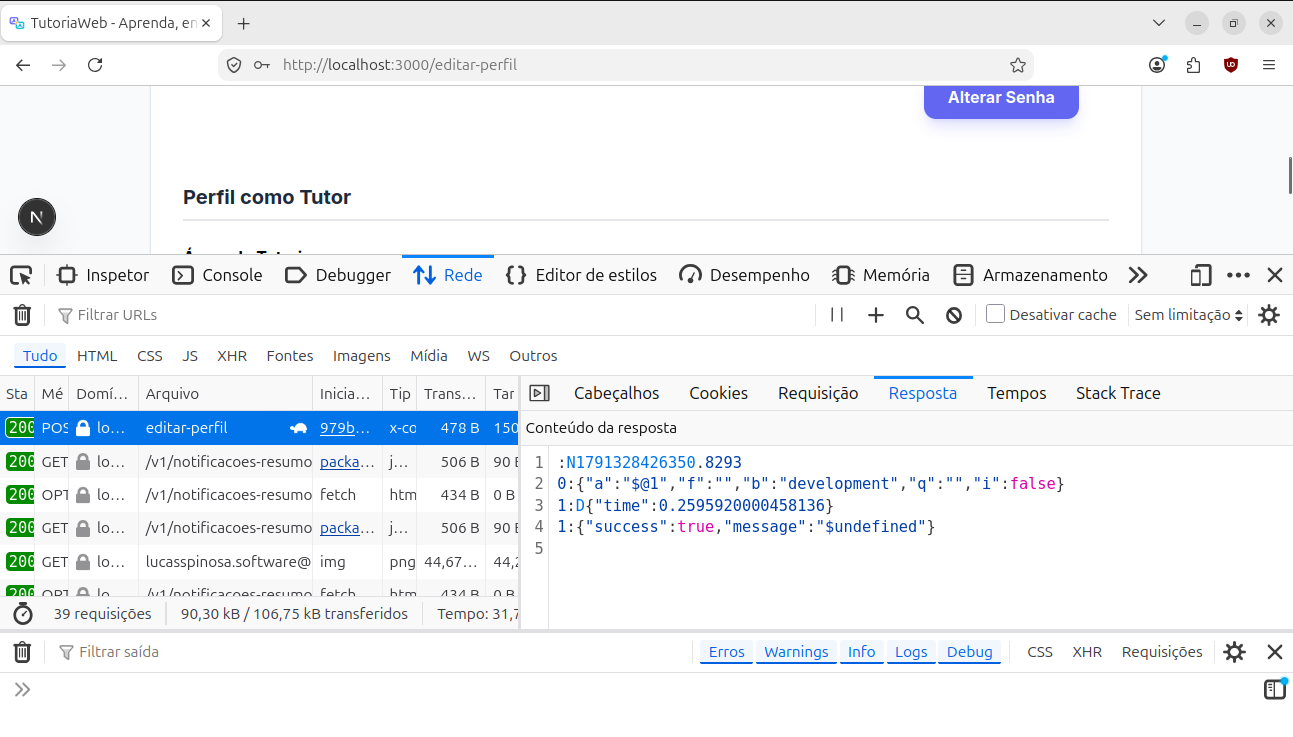
\includegraphics[width=1.9\textwidth, height=0.90\textheight, keepaspectratio]{figuras/ocultaçãoResponse.png}
    
    
        Fonte: Autoria própria.
        
        \vspace{0.2cm}
            
        \label{fig:ocultaçãoResponse}
    \end{figure}
\end{landscape}

Essa mudança na arquitetura causou a criação da pasta \textit{actions} dentro da pasta \textit{services}, de modo que \textit{actions} contém arquivos com as \textit{Server Actions} e \textit{services} contém as funções de requisição ao \textit{backend}. Foi também criada a pasta \textit{types}, que contém interfaces de dados usados no \textit{frontend} da aplicação, como respostas das requisições e estruturas de corpos de requisições. Uma representação visual da arquitetura final pode ser observada na Figura \ref{fig:ArquiteturaFinal}.

\begin{figure}[h!]
    \centering
    \caption{Representação Arquitetural Final.} 
    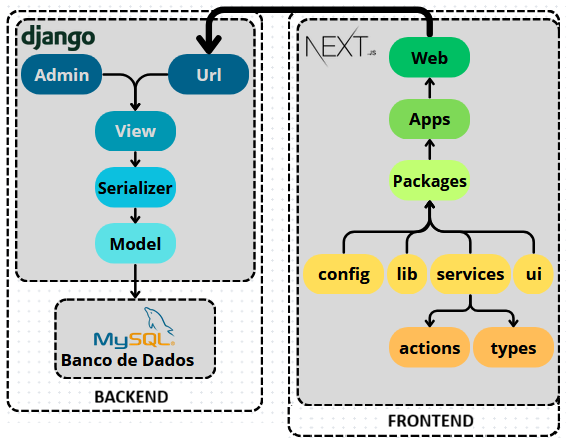
\includegraphics[width=0.70\textwidth]{figuras/Arquitetura Final.png}


    Fonte: Autoria própria.
    
    \vspace{0.2cm}
        
    \label{fig:ArquiteturaFinal}
\end{figure}

\section[Desenvolvimento da Aplicação]{Desenvolvimento da Aplicação}
\label{sec:desenvolvimento}

Durante o desenvolvimento da aplicação, optou-se pela divisão de cada US entre \textit{backend} e \textit{frontend}, sendo criadas as tarefas de cada área para cada US no Trello, conforme pode ser observado nas Figuras \ref{fig:trelloFront} e \ref{fig:trelloBack}.

\clearpage

\begin{figure}
    \centering
    \caption{Tarefa de \textit{frontend} no Trello.} 
    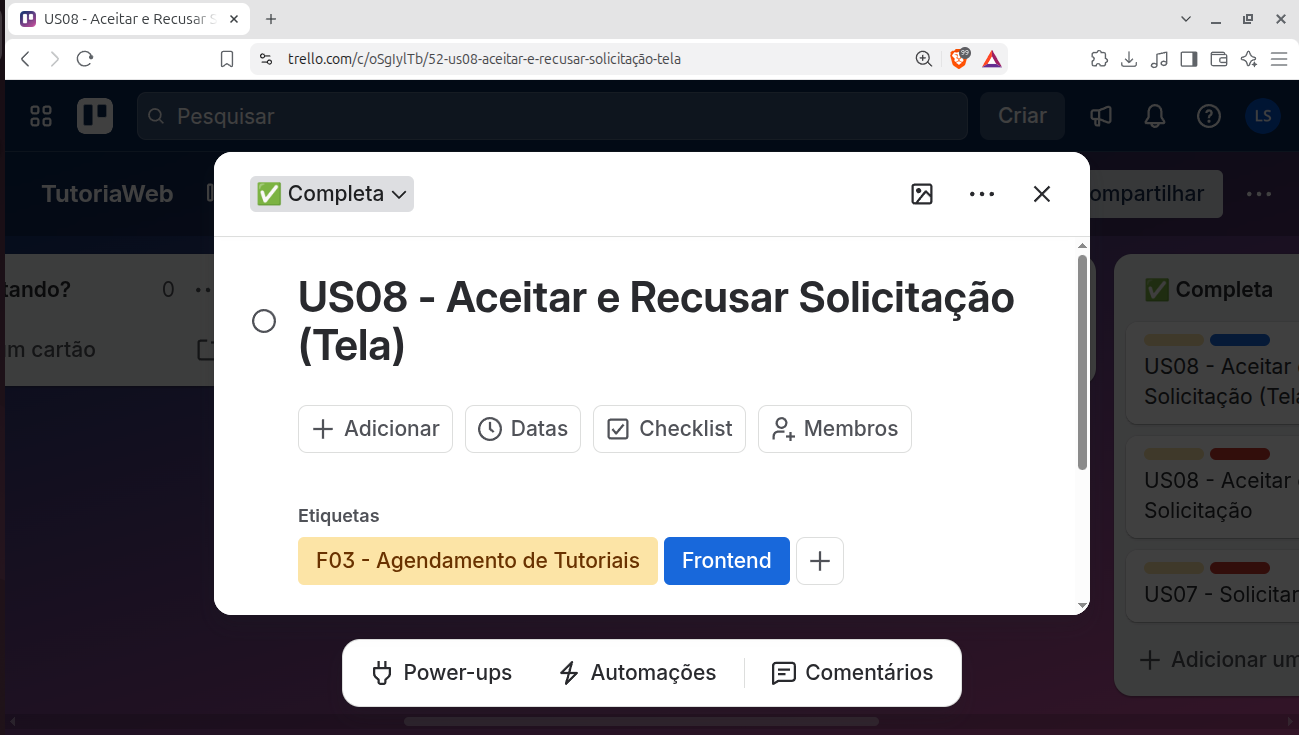
\includegraphics[width=0.90\textwidth]{figuras/trelloFront.png}

    Fonte: Autoria própria.
    
    \vspace{0.2cm}
        
    \label{fig:trelloFront}
\end{figure}

\begin{figure}
    \centering
    \caption{Tarefa de \textit{backend} no Trello.} 
    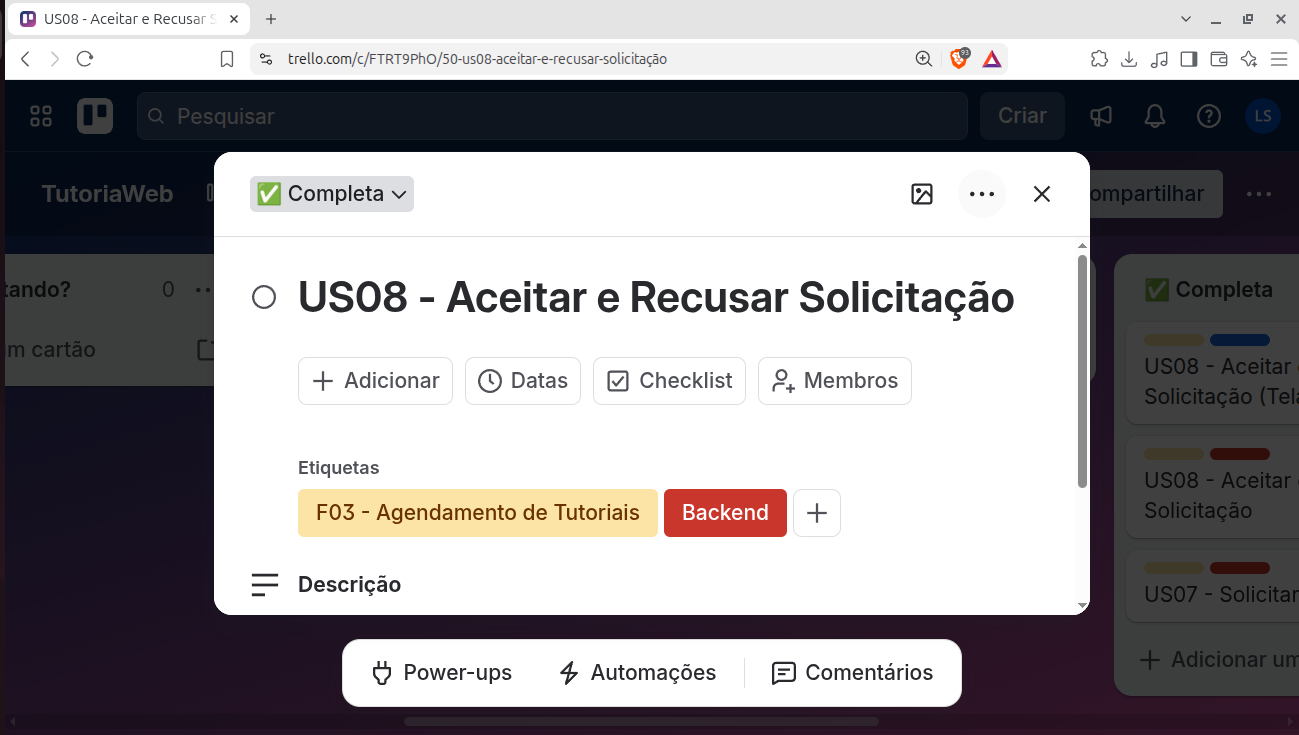
\includegraphics[width=0.90\textwidth]{figuras/trelloBack.png}

    Fonte: Autoria própria.
    
    \vspace{0.2cm}
        
    \label{fig:trelloBack}
\end{figure}

Foram realizadas reuniões de 19h até 22h de segunda à sexta no Discord para desenvolvimento em conjunto, sendo utilizado o método Pomodoro a fim de se obter melhor produtividade. O método Pomodoro é fundamentado na estratégia que se apoia em períodos de tempo delimitados, nos quais se concentra a atenção na realização de uma determinada atividade, intercalados por intervalos de descanso \cite{rodrigues2023focus}. 

Os períodos de tempo foram definidos em 40 minutos de desenvolvimento e 20 minutos de descanso, sendo considerados ideais baseado em experiências empíricas pelos autores. Considerando o horário de início e término das reuniões, o tempo de desenvolvimento foi de 2 horas por reunião.

Ocorreram atrasos na entrega de algumas funcionalidades, visto que houveram reuniões exclusivamente utilizadas para correções de \textit{bugs} no código. Entretanto, os autores utilizaram essa metodologia por se adequar à realidade da vida cotidiana dos mesmos, que estagiavam de manhã e frequentavam aulas à tarde. Além disso, os intervalos de descanso possibilitavam voltar ao desenvolvimento com mais foco e energia.

O repositório do \textit{backend} está disponível no seguinte endereço virtual: \url{https://github.com/TutoriaWebApp/backend}.

O repositório do \textit{frontend} está disponível no seguinte endereço virtual: \url{https://github.com/TutoriaWebApp/frontend}.

O quadro do Trello exige criação de conta para ser visualizado, e um convite para sua visualização está disponível no seguinte endereço virtual:  \url{https://trello.com/invite/b/692f73a8eae6979484e7e1e4/ATTI1d25182b917b29f2c5164cd540d66020EE133345/tutoriaweb}.

\subsection[Funcionalidade 1: Autenticação]{Funcionalidade 1: Autenticação}

\subsubsection[US01: \textit{Login}]{US01: \textit{Login}}

A estimativa inicial para o desenvolvimento da US01 era na Semana 1, em conjunto com a US02, de 08 a 14 de março. Tanto o \textit{backend} quanto o \textit{frontend} foram em sua grande parte desenvolvidos nesse prazo, com refatorações no \textit{frontend} em 19 de março para inclusão de responsividade para dispositivos móveis, no dia 21 de março para implementar o uso de \textit{Server Actions}, no dia 22 de março para inclusão de um banner informativo sobre o uso de \textit{cookies} na aplicação, em conformidade com a LGPD (Lei Geral de Proteção de Dados) e no dia 27 de março para mudança no formulário para utilização das bibliotecas React Hook Form e Zod, que serão explicadas na Subseção \ref{sec:us20}.

No \textit{backend} a autenticação se utiliza de uma classe abstrata do modelo de Usuário do DRF, adaptada e costumizada para as regras de negócios da aplicação. O modelo ``UsuarioModel'' estende as classes ``AbstractBaseUser'' e ``PermissionMixin'', além de criar um ``UsuarioManager'' que o DRF utiliza para definir regras de criação, atualização deste Usuário base e também para o ``superuser''. Desta forma foi possível aproveitar funções já implementadas no \textit{framework}, como criptografia de senha, registro de \textit{login} e autenticação via JWT, utilizando o pacote do DRF chamado ``djangorestframework-simplejwt''.

Conforme mencionado acima, foi realizado a responsividade para dispositivos móveis nesta e nas demais telas e componentes visuais da aplicação. As versões \textit{mobile}, \textit{tablet} e \textit{desktop} da tela podem ser observadas nas Figuras \ref{fig:loginMobile}, \ref{fig:loginTablet} e  \ref{fig:loginDesktop}.

A partir de página de \textit{Login} foi implementada uma otimização na forma de renderização das telas utilizando-se \textit{Server Components} e \textit{Client Components}. \textit{Server Components} são componentes de UI renderizados no servidor e enviados ao cliente (navegador) \cite{nextjs2026components}. \textit{Client Components} são componentes de UI renderizados no cliente, sendo recomendados quando se deseja interatividade com o usuário \cite{nextjs2026components}.

Utilizar \textit{Server Components} resulta em benefícios para o usuário, pois reduz o tempo de carregamento da página ao enviar HTML (\textit{HyperText Markup Language}) estático para o cliente, evitando o envio de código JavaScript para a renderização de componentes visuais. A estratégia utilizada pelos autores foi colocar o máximo possível de elementos de UI como \textit{Server Components}, deixando apenas partes interativas como \textit{Client Components}. No \textit{login}, a maior parte da página é \textit{Server Component}, sendo apenas o formulário de \textit{login} um \textit{Client Component}.

\clearpage

\begin{landscape}
    \setlength{\oddsidemargin}{\evensidemargin}
    \numeracaoPaisagem
    \begin{figure}[H]
        \centering
        \caption{Página de \textit{Login} em \textit{mobile}.} 
        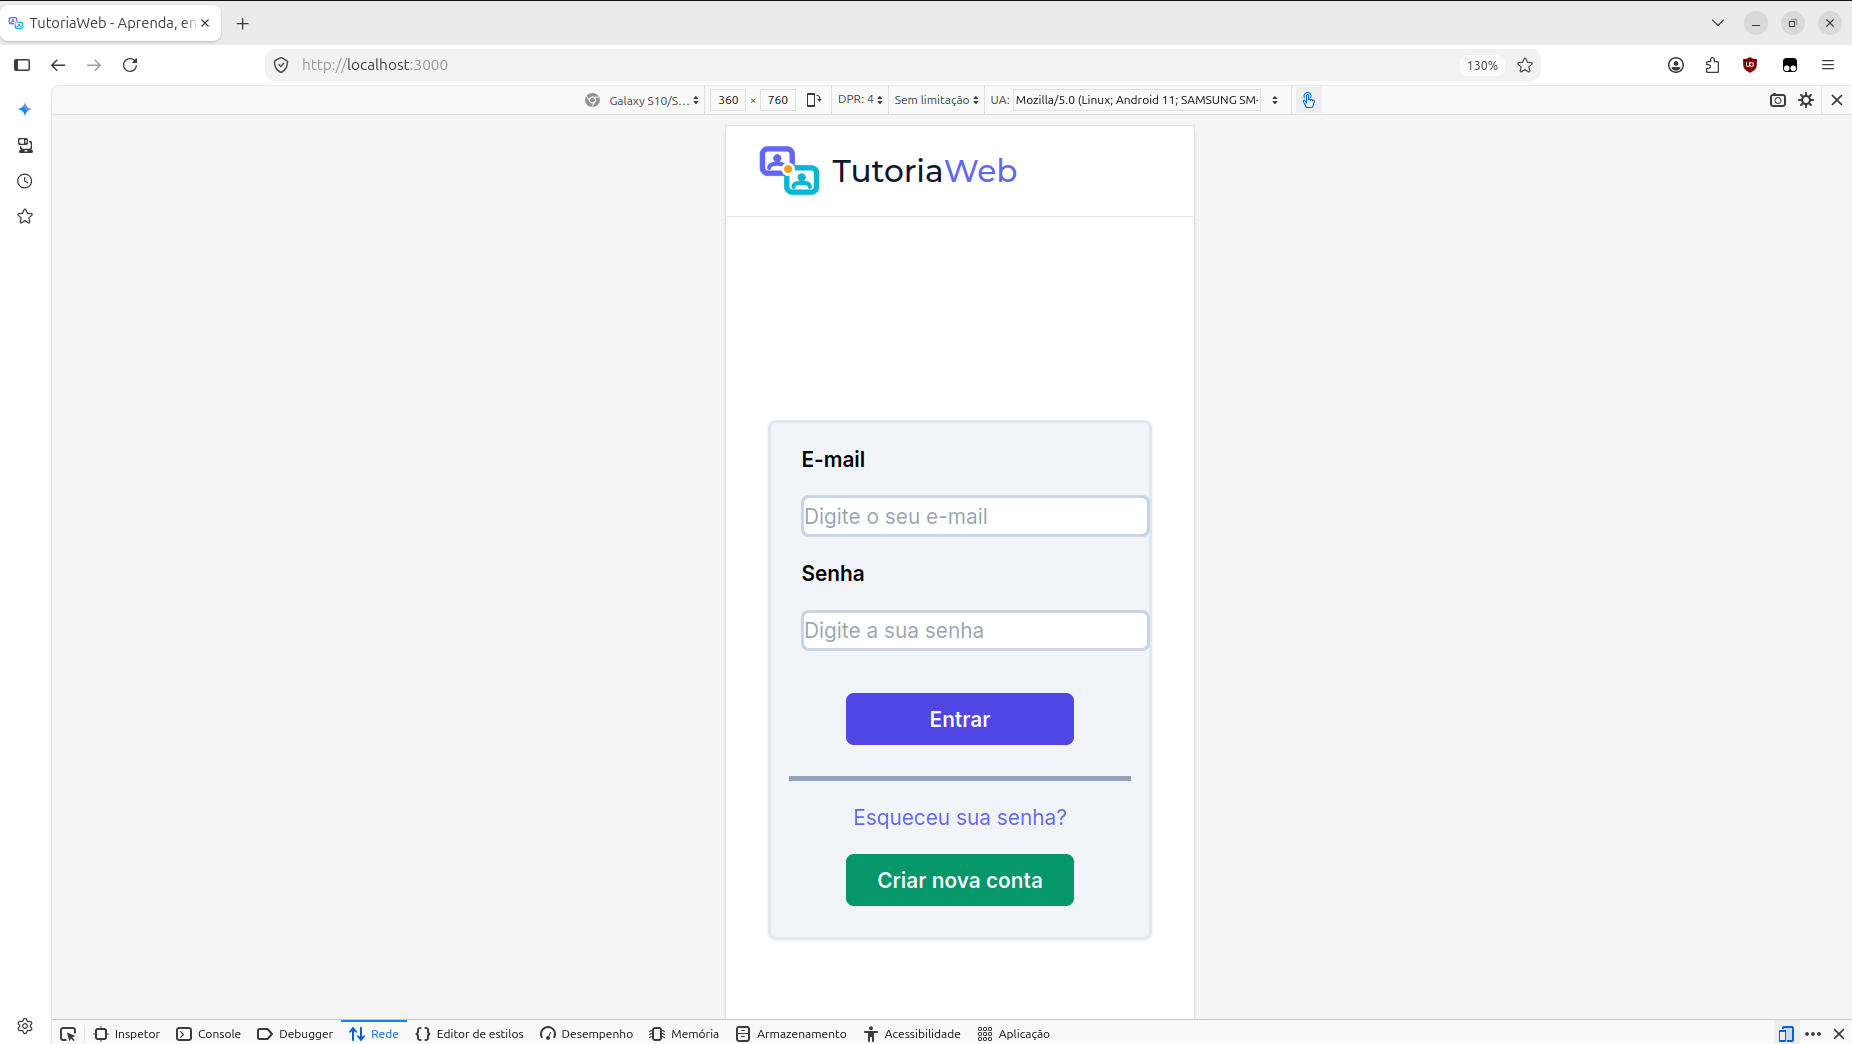
\includegraphics[width=1.9\textwidth, height=0.90\textheight, keepaspectratio]{figuras/loginMobile.png}
    
    
        Fonte: Autoria própria.
        
        \vspace{0.2cm}
            
        \label{fig:loginMobile}
    \end{figure}
\end{landscape}

\clearpage

\begin{landscape}
    \setlength{\oddsidemargin}{\evensidemargin}
    \numeracaoPaisagem
    \begin{figure}[H]
        \centering
        \caption{Página de \textit{Login} em \textit{tablet}.} 
        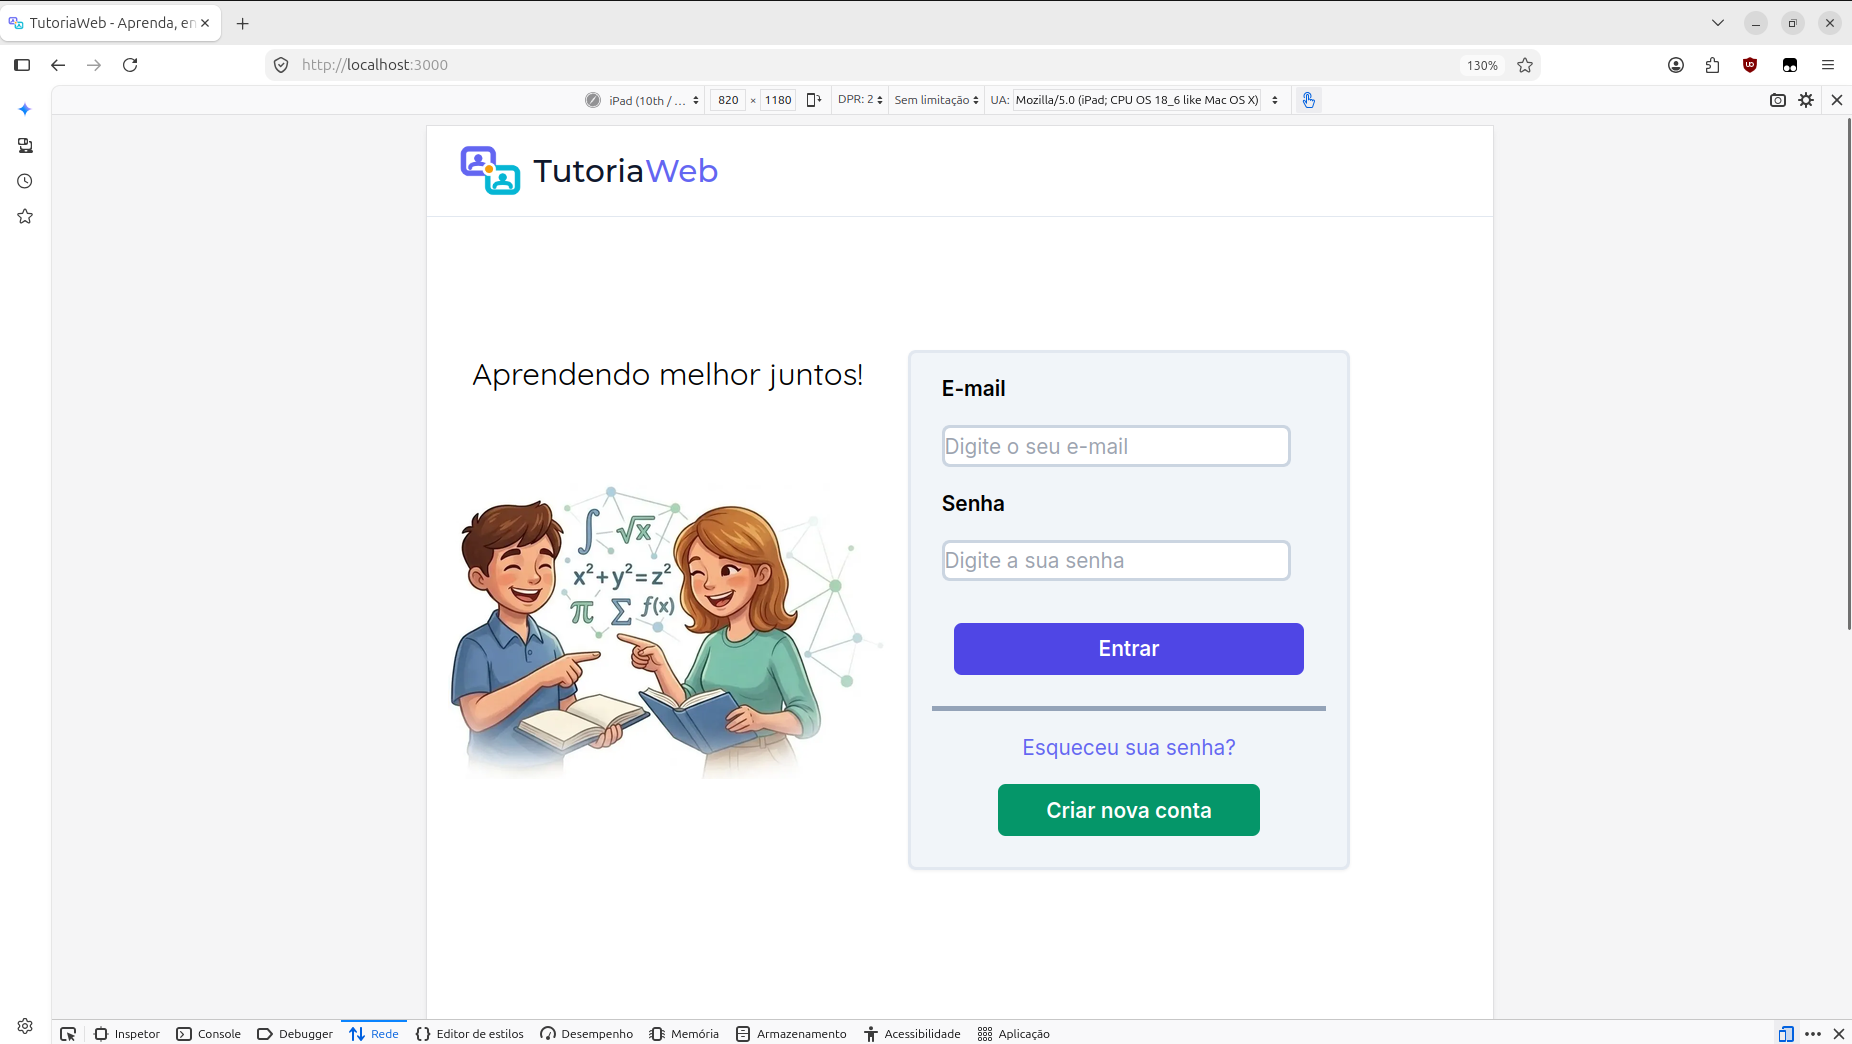
\includegraphics[width=1.9\textwidth, height=0.90\textheight, keepaspectratio]{figuras/loginTablet.png}
    
    
        Fonte: Autoria própria.
        
        \vspace{0.2cm}
            
        \label{fig:loginTablet}
    \end{figure}
\end{landscape}


\clearpage

\begin{landscape}
    \setlength{\oddsidemargin}{\evensidemargin}
    \numeracaoPaisagem
    \begin{figure}[H]
        \centering
        \caption{Página de \textit{Login} em \textit{Desktop}.} 
        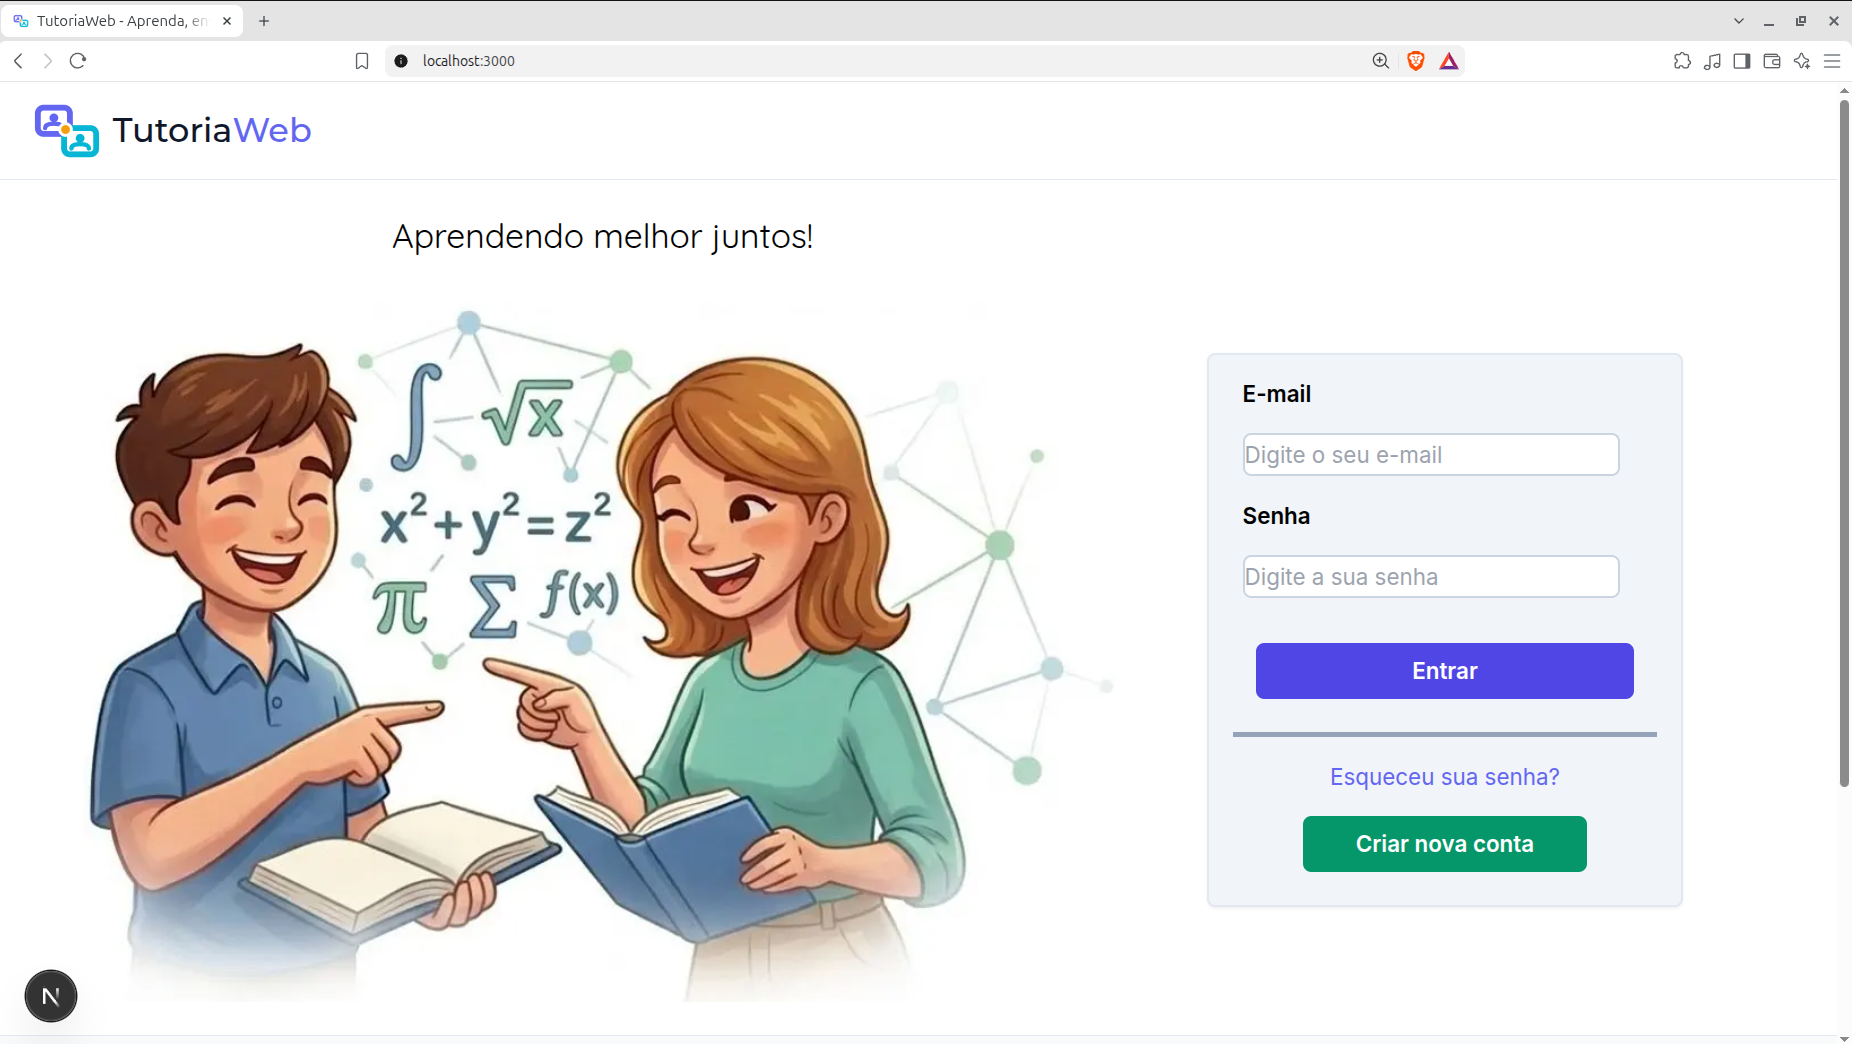
\includegraphics[width=1.9\textwidth, height=0.90\textheight, keepaspectratio]{figuras/loginDesktop.png}
    
    
        Fonte: Autoria própria.
        
        \vspace{0.2cm}
            
        \label{fig:loginDesktop}
    \end{figure}
\end{landscape}

Atendendo ao RNF 02 descrito na Subseção \ref{requisitosNaoFuncionais}, é feita validação dos campos assim que o usuário começa a preenchê-los. Isso ocorre em todos os outros formulários da aplicação. Na página de \textit{login} especificamente, caso o usuário informe um e-mail com formato inválido, o formulário exibe a mensagem de erro ``E-mail inválido''. Se o usuário informa o e-mail e tenta realizar \textit{login} sem informar a senha, a mensagem ``A senha é obrigatória'' é apresentada. Caso o usuário tente fazer \textit{login} com e-mail ou senha errados, é exibida a mensagem ``Credenciais inválidas'', não sendo informado qual dos campos está incorreto por razões de segurança. Essas mensagens podem ser observadas nas Figuras \ref{fig:loginErroEmail}, \ref{fig:loginErroSenha} e  \ref{fig:loginErroValorErrado}.

A aplicação utiliza \textit{cookies} de autenticação em sua navegação. De acordo com \citeonline{ANPDcookies}, a LGPD considera esses \textit{cookies} como necessários,  não exigindo consentimento prévio do usuário e devendo a aplicação apenas informar o usuário sobre a existência e finalinalidade deles. Para atender esse requisito, é exibido um \textit{banner} informativo na primeira vez que a aplicação é acessada. O \textit{banner} só é removido da tela quando o botão de declaração de ciência é clicado. O \textit{banner} pode ser observado na Figura \ref{fig:loginBanner}.

\clearpage

\begin{landscape}
    \setlength{\oddsidemargin}{\evensidemargin}
    \numeracaoPaisagem
    \begin{figure}[H]
        \centering
        \caption{Mensagem de erro para e-mail inválido.} 
        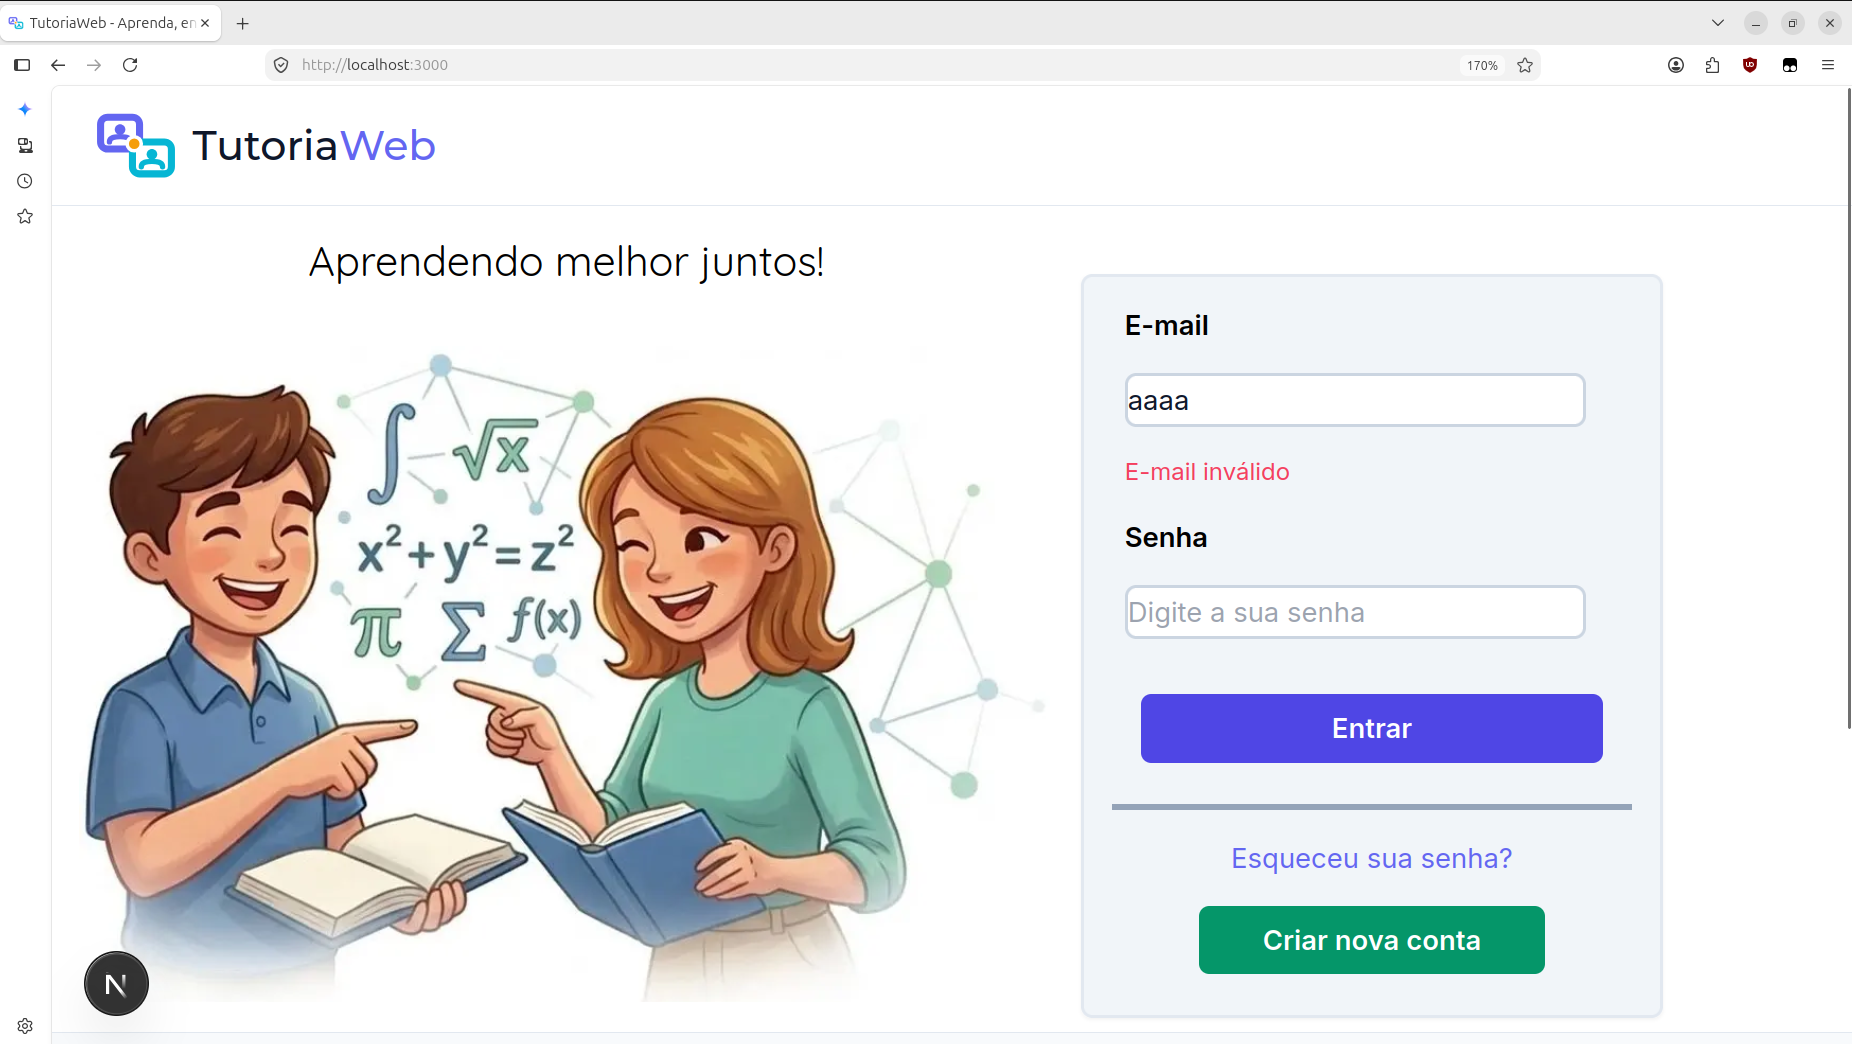
\includegraphics[width=1.9\textwidth, height=0.90\textheight, keepaspectratio]{figuras/loginErroEmail.png}
    
    
        Fonte: Autoria própria.
        
        \vspace{0.2cm}
            
        \label{fig:loginErroEmail}
    \end{figure}
\end{landscape}

\clearpage

\begin{landscape}
    \setlength{\oddsidemargin}{\evensidemargin}
    \numeracaoPaisagem
    \begin{figure}[H]
        \centering
        \caption{Mensagem de erro para senha em branco.} 
        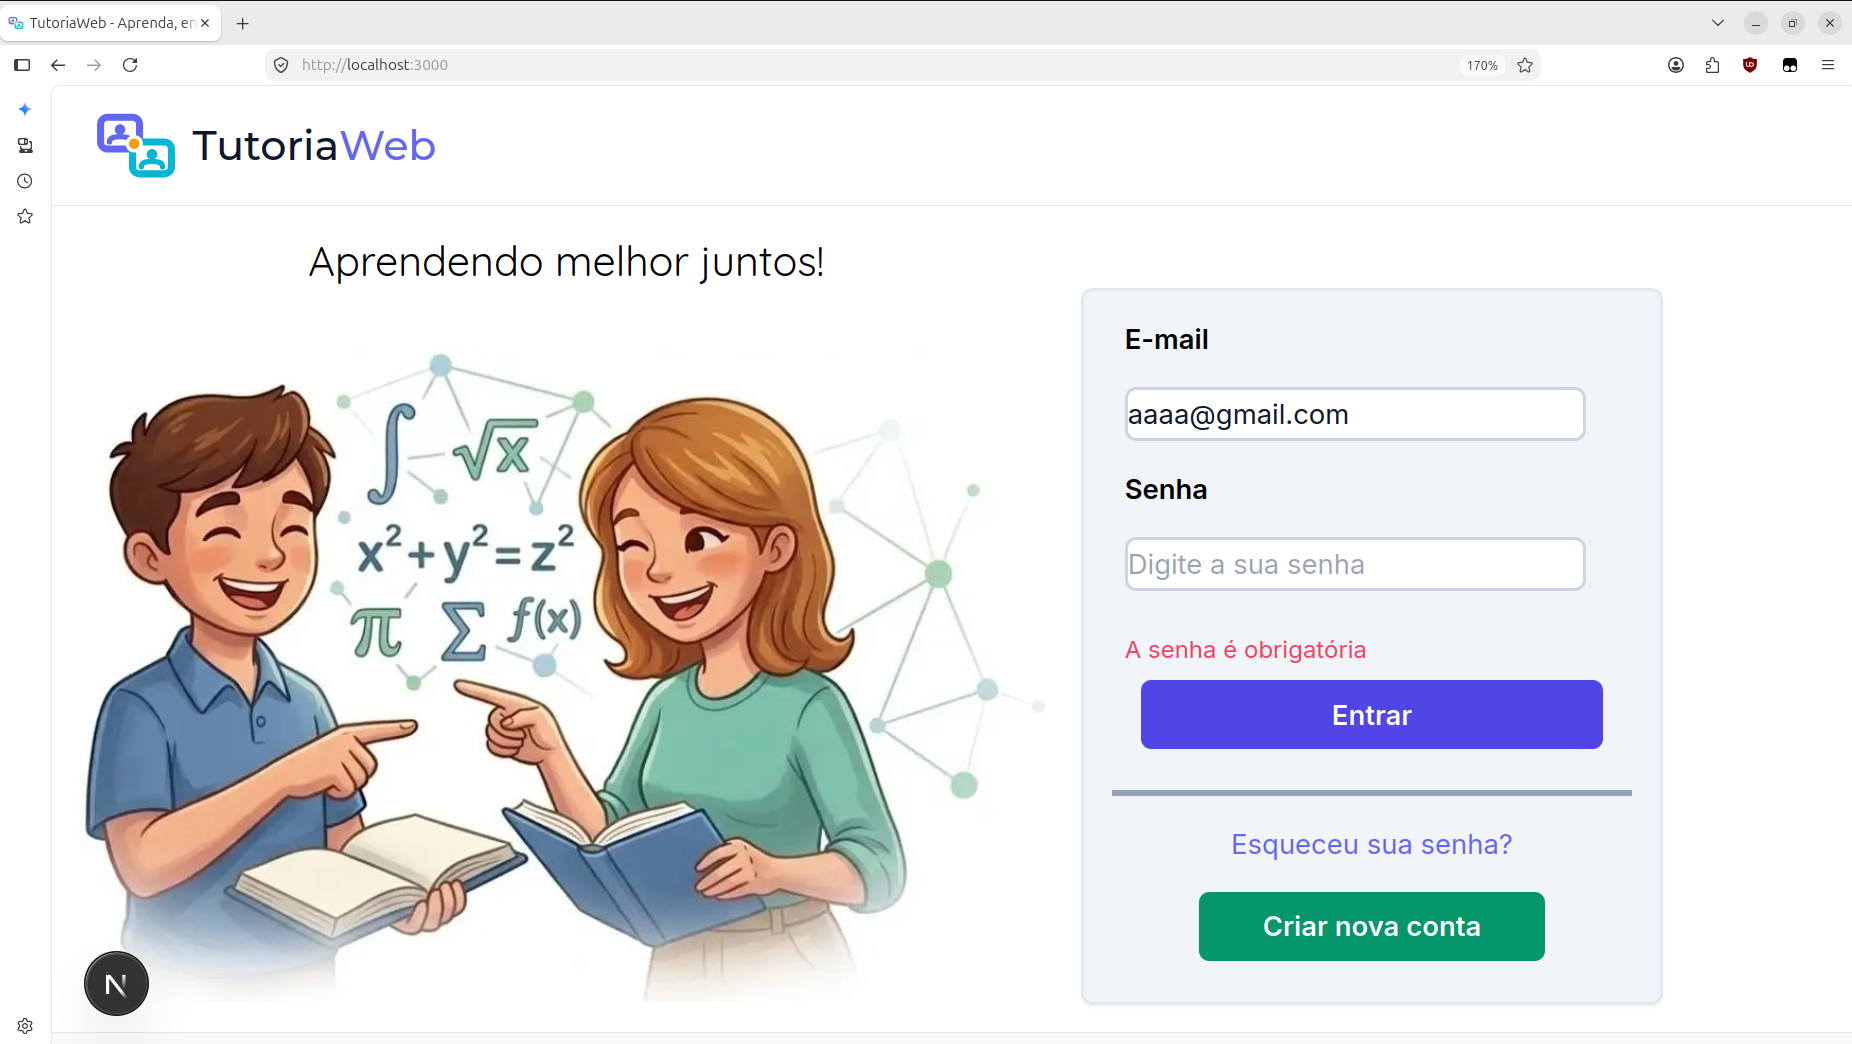
\includegraphics[width=1.9\textwidth, height=0.90\textheight, keepaspectratio]{figuras/loginErroSenha.png}
    
    
        Fonte: Autoria própria.
        
        \vspace{0.2cm}
            
        \label{fig:loginErroSenha}
    \end{figure}
\end{landscape}


\clearpage

\begin{landscape}
    \setlength{\oddsidemargin}{\evensidemargin}
    \numeracaoPaisagem
    \begin{figure}[H]
        \centering
        \caption{Mensagem de erro para valores incorretos.} 
        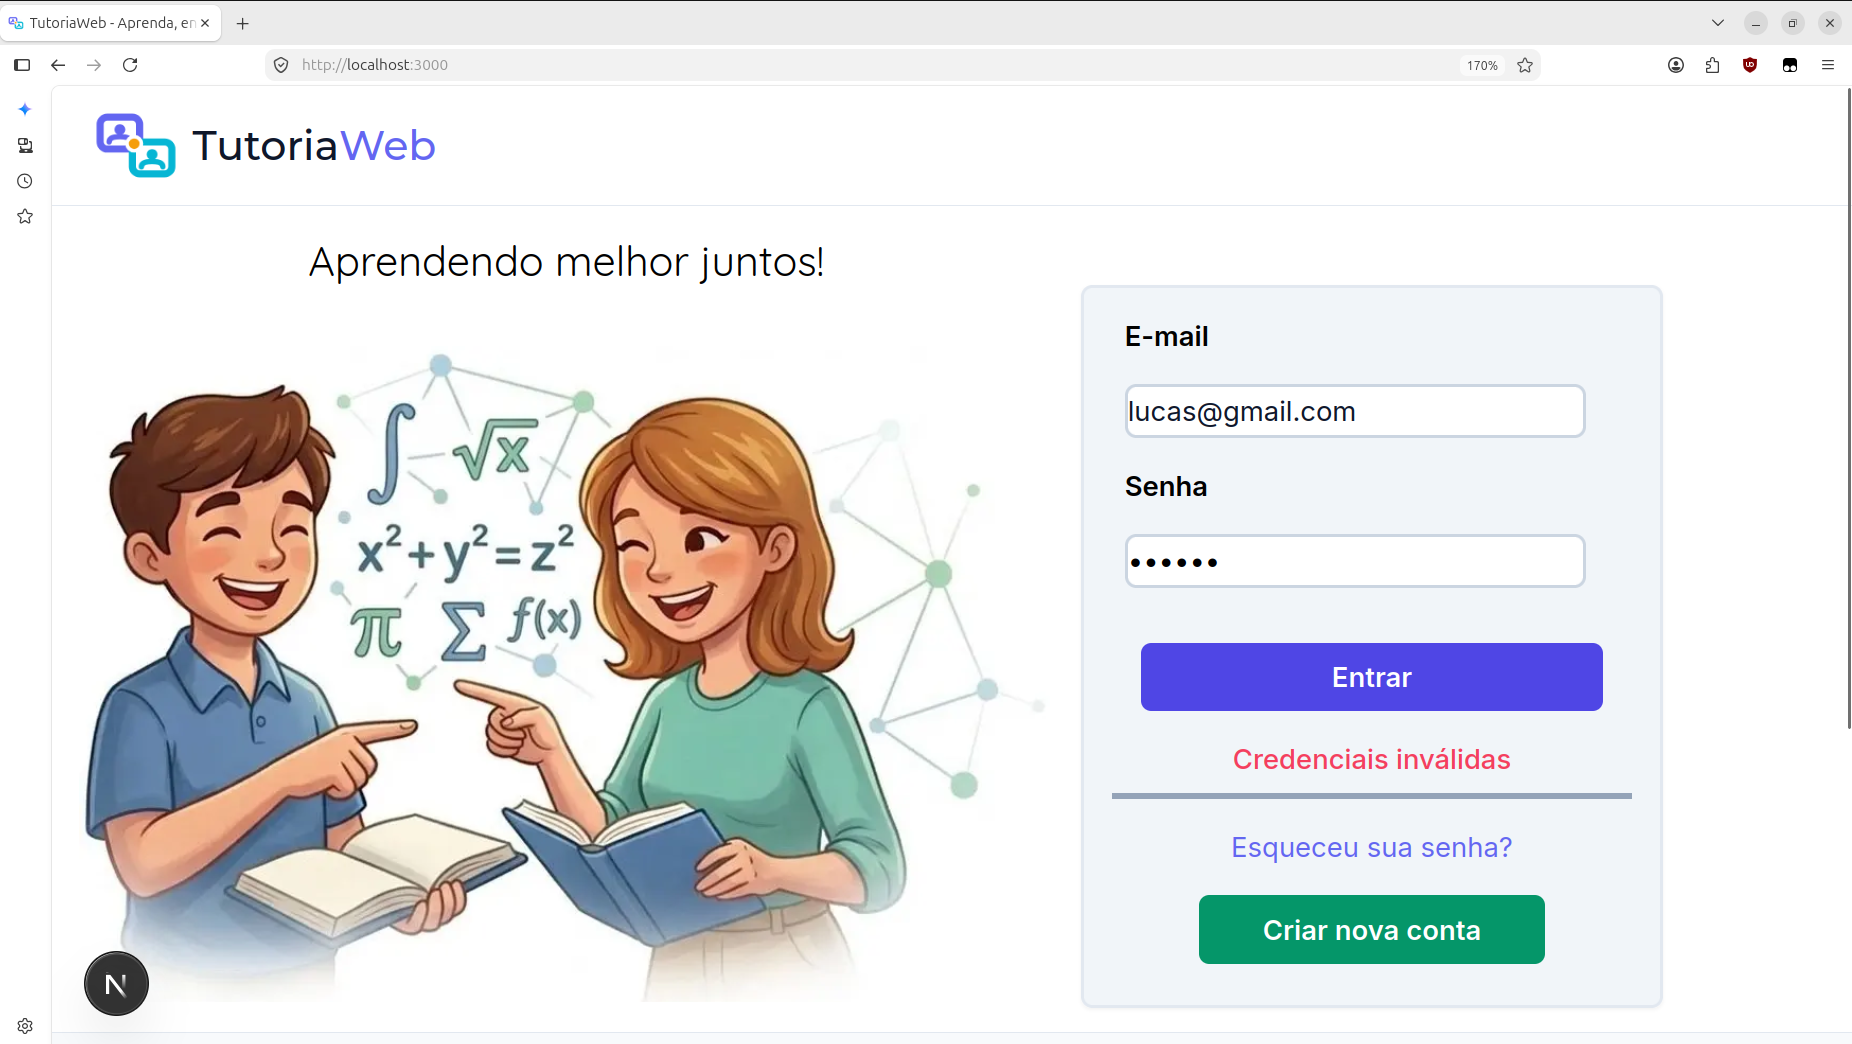
\includegraphics[width=1.9\textwidth, height=0.90\textheight, keepaspectratio]{figuras/loginErroValorErrado.png}
    
    
        Fonte: Autoria própria.
        
        \vspace{0.2cm}
            
        \label{fig:loginErroValorErrado}
    \end{figure}
\end{landscape}

\begin{landscape}
    \setlength{\oddsidemargin}{\evensidemargin}
    \numeracaoPaisagem
    \begin{figure}[H]
        \centering
        \caption{Banner informativo sobre o uso de \textit{cookies}.} 
        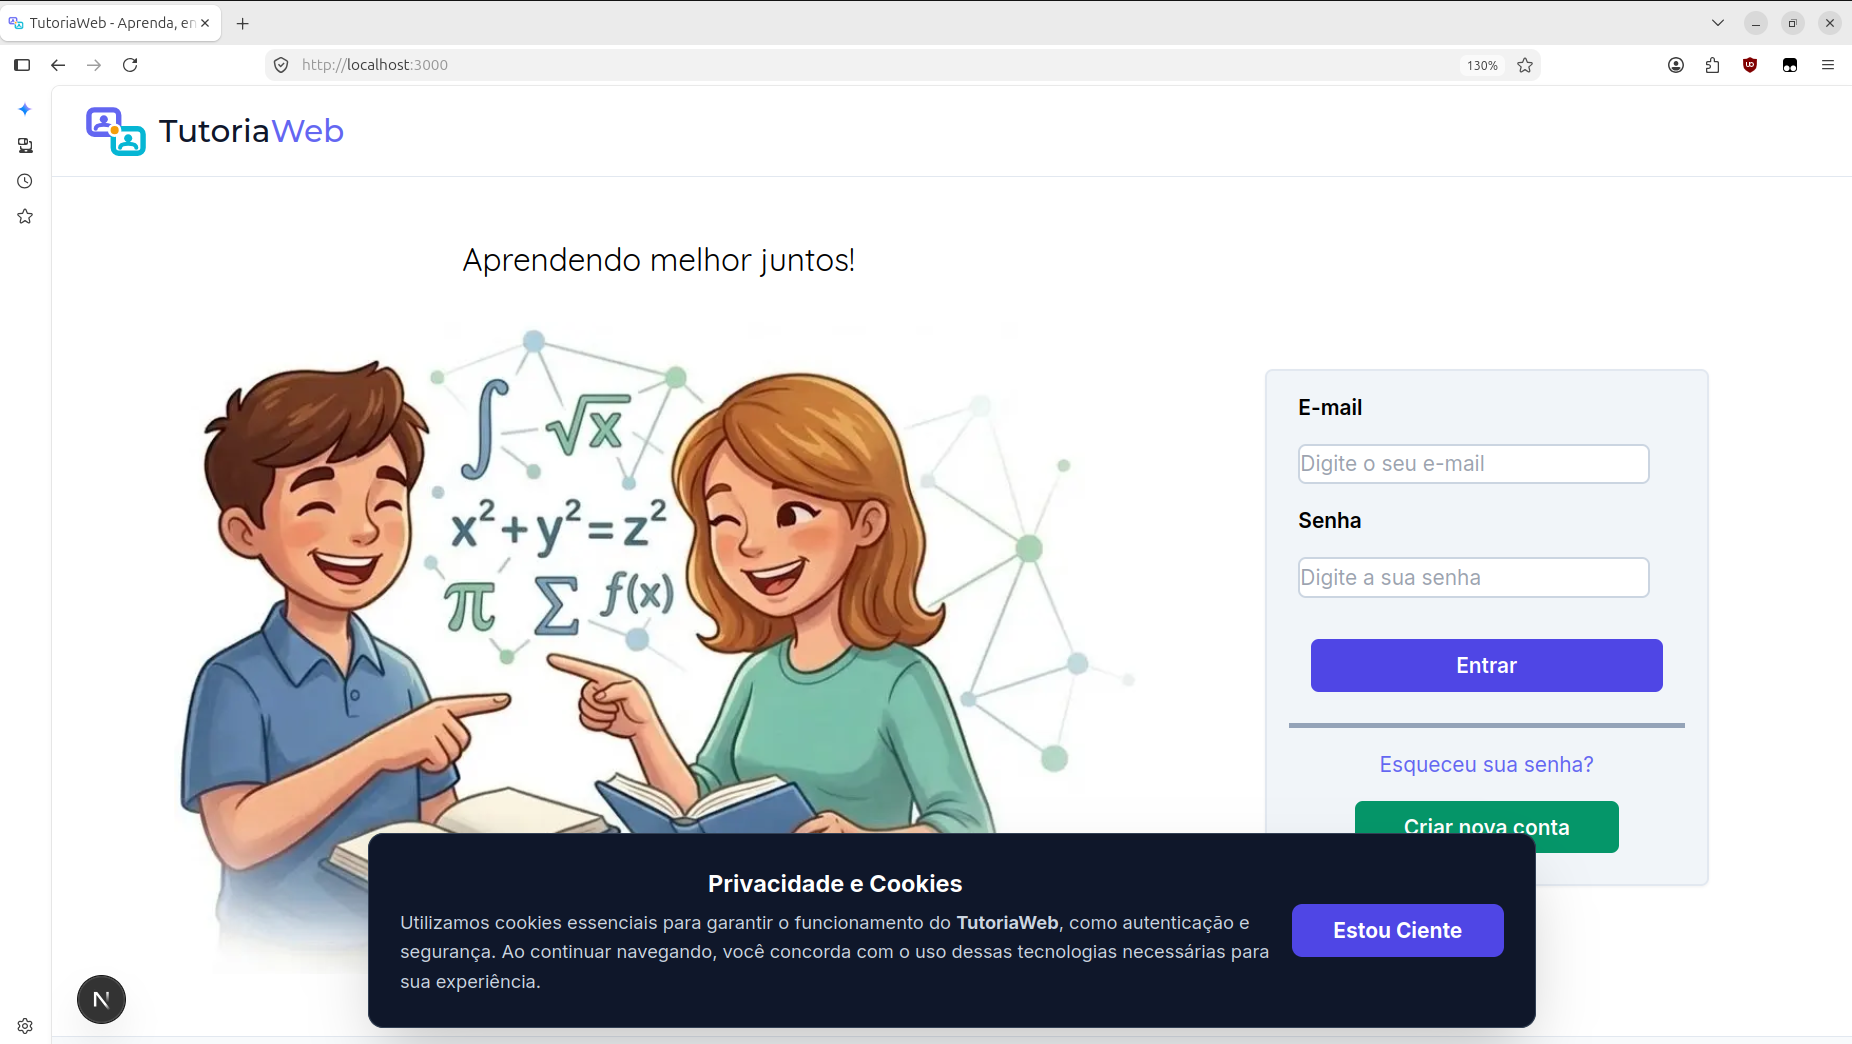
\includegraphics[width=1.9\textwidth, height=0.90\textheight, keepaspectratio]{figuras/loginBanner.png}
    
    
        Fonte: Autoria própria.
        
        \vspace{0.2cm}
            
        \label{fig:loginBanner}
    \end{figure}
\end{landscape}

Caso o usuário informe credenciais corretas e faça a requisição, o \textit{backend} recebe os dados e realiza duas verificações: se o e-mail está registrado no banco de dados e se a senha enviada, quando criptografada, coincide com a senha criptografada armazenada com o do registro do e-mail. 

Caso verdadeiro, o \textit{backend} envia os dois \textit{tokens} que são salvos como \textit{cookies} no navegador: um \textit{token} de acesso (\textit{access\_token}), com duração de 20 minutos, e um \textit{token} de renovação (\textit{refresh\_token}), usado para renovar o \textit{token} de acesso, com duração de 2 horas, atendendo ao RNF 05 e ao RNF 06. Dessa maneira, caso o usuário navegue para uma página que exija autenticação ou realize uma requisição, caso o \textit{token} de acesso esteja expirado, o \textit{token} de renovação é usado a operação prossegue normalmente.

Caso o \textit{token} de renovação também esteja expirado, o usuário é redirecionado para a página de \textit{login}, mas com uma \textit{modal} informando-o que sua sessão expirou, orientando-o a realizar a conexão na aplicação novamente. A \textit{modal} pode ser observada na Figura \ref{fig:modalTokenExpirado}.

O armazenamento dos \textit{tokens} como \textit{cookies}, utilizando o método de \textit{Cookies HttpOnly}, onde o próprio navegador do usuário lê o cabeçalho enviado pelo \textit{backend} e guarda o \textit{cookie} de forma automática e segura, foi a única dificuldade notável no desenvolvimento do \textit{frontend} e \textit{backend}, visto que os autores até então desconheciam como isso era realizado, sendo essa dúvida solucianada através de pesquisas sobre o assunto na Internet.

\begin{landscape}
    \setlength{\oddsidemargin}{\evensidemargin}
    \numeracaoPaisagem
    \begin{figure}[H]
        \centering
        \caption{\textit{Modal} informativo sobre a expiração da sessão.} 
        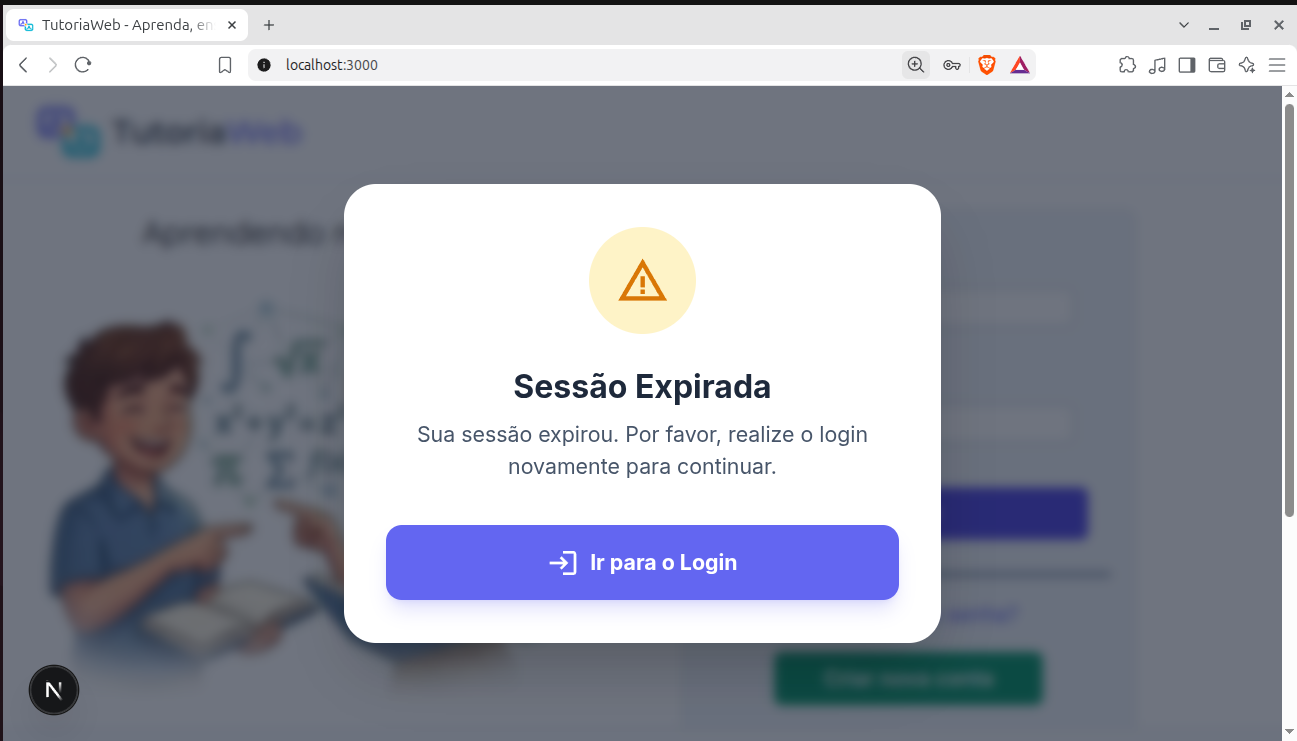
\includegraphics[width=1.9\textwidth, height=0.90\textheight, keepaspectratio]{figuras/modalTokenExpirado.png}
    
    
        Fonte: Autoria própria.
        
        \vspace{0.2cm}
            
        \label{fig:modalTokenExpirado}
    \end{figure}
\end{landscape}

\subsubsection[US20: {Criar Conta}]{US20: Criar Conta}
\label{sec:us20}

Uma funcionalidade que está relacionada ao \textit{login} e não havia sido listada na Subseção \ref{historias-usuario} é a criação de conta, se tornando assim a US20. O desenvolvimento do \textit{backend} iniciou-se com o \textit{endpoint} para criação de usuário em 14 de outubro de 2025, concluindo em 20 de outubro do mesmo ano. Porém, houve refatorações arquiteturais e inclusões posteriores principalmente na semana de 22 a 28 de março de 2026. 

O \textit{frontend} da criação de conta começou a ser desenvolvido em 16 de março e foi concluída em 10 de junho. O grande período de desenvolvimento se deve ao fato dessa funcionalidade ter sido feita em paralelo com outras US, que foram se tornando mais prioritárias após a criação de um usuário como aprendiz ter sido concluída, e também ao \textit{backend} dessa funcionalidade ter sido completado em partes, também em paralelo com outras funcionalidades. 

A página possui duas etapas, sendo a primeira o cadastro de informações comuns à aprendiz e tutores, como foto de perfil, e-mail e senha, e a segunda exclusivamente para cadastro de dados para o perfil como tutor. Caso os dados da segunda etapa também sejam preenchidos, o usuário já é registrado como um tutor assim que o processo é concluído. Ambas as etapas podem ser observadas nas Figuras \ref{fig:criarConta1} e \ref{fig:criarConta2}.

No preenchimento de dados de tutor, foi implementada a regra de negócio do usuário obrigatoriamente ter que preencher uma área e especialidade de conhecimento, além de uma disponibilidade, devendo ter ao menos uma área e especialidade e uma disponibilidade para se tornar um tutor. A seleção de disponibilidade apresenta os dias da semana e intervalos de tempo de uma hora, abrangendo os horários de um dia inteiro. Tudo isso é feito através de \textit{modais}, que podem ser observadas nas Figuras \ref{fig:modalArea} e \ref{fig:modalAgenda}.

\clearpage

\begin{landscape}
    \setlength{\oddsidemargin}{\evensidemargin}
    \numeracaoPaisagem
    \begin{figure}[H]
        \centering
        \caption{Etapa de cadastro de informações comuns.} 
        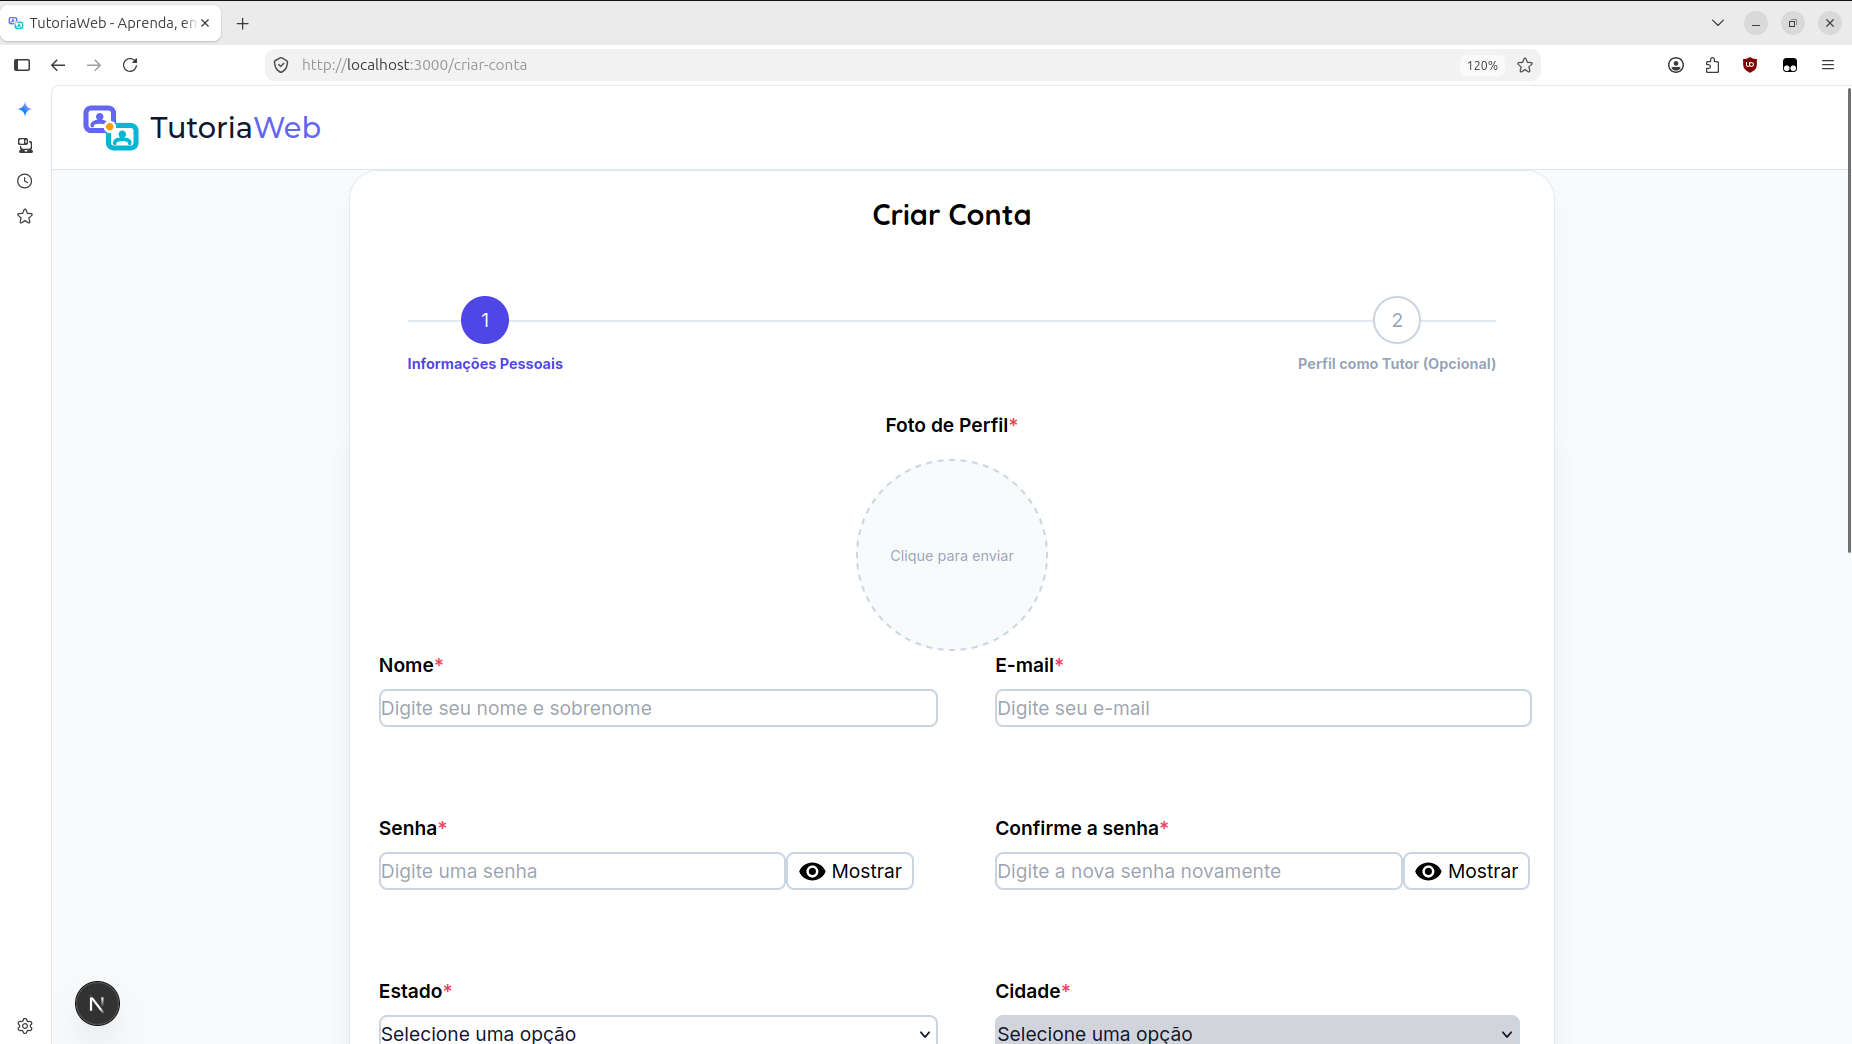
\includegraphics[width=1.9\textwidth, height=0.90\textheight, keepaspectratio]{figuras/criarConta1.png}
    
    
        Fonte: Autoria própria.
        
        \vspace{0.2cm}
            
        \label{fig:criarConta1}
    \end{figure}
\end{landscape}

\clearpage

\begin{landscape}
    \setlength{\oddsidemargin}{\evensidemargin}
    \numeracaoPaisagem
    \begin{figure}[H]
        \centering
        \caption{Etapa de cadastro de informações como tutor.} 
        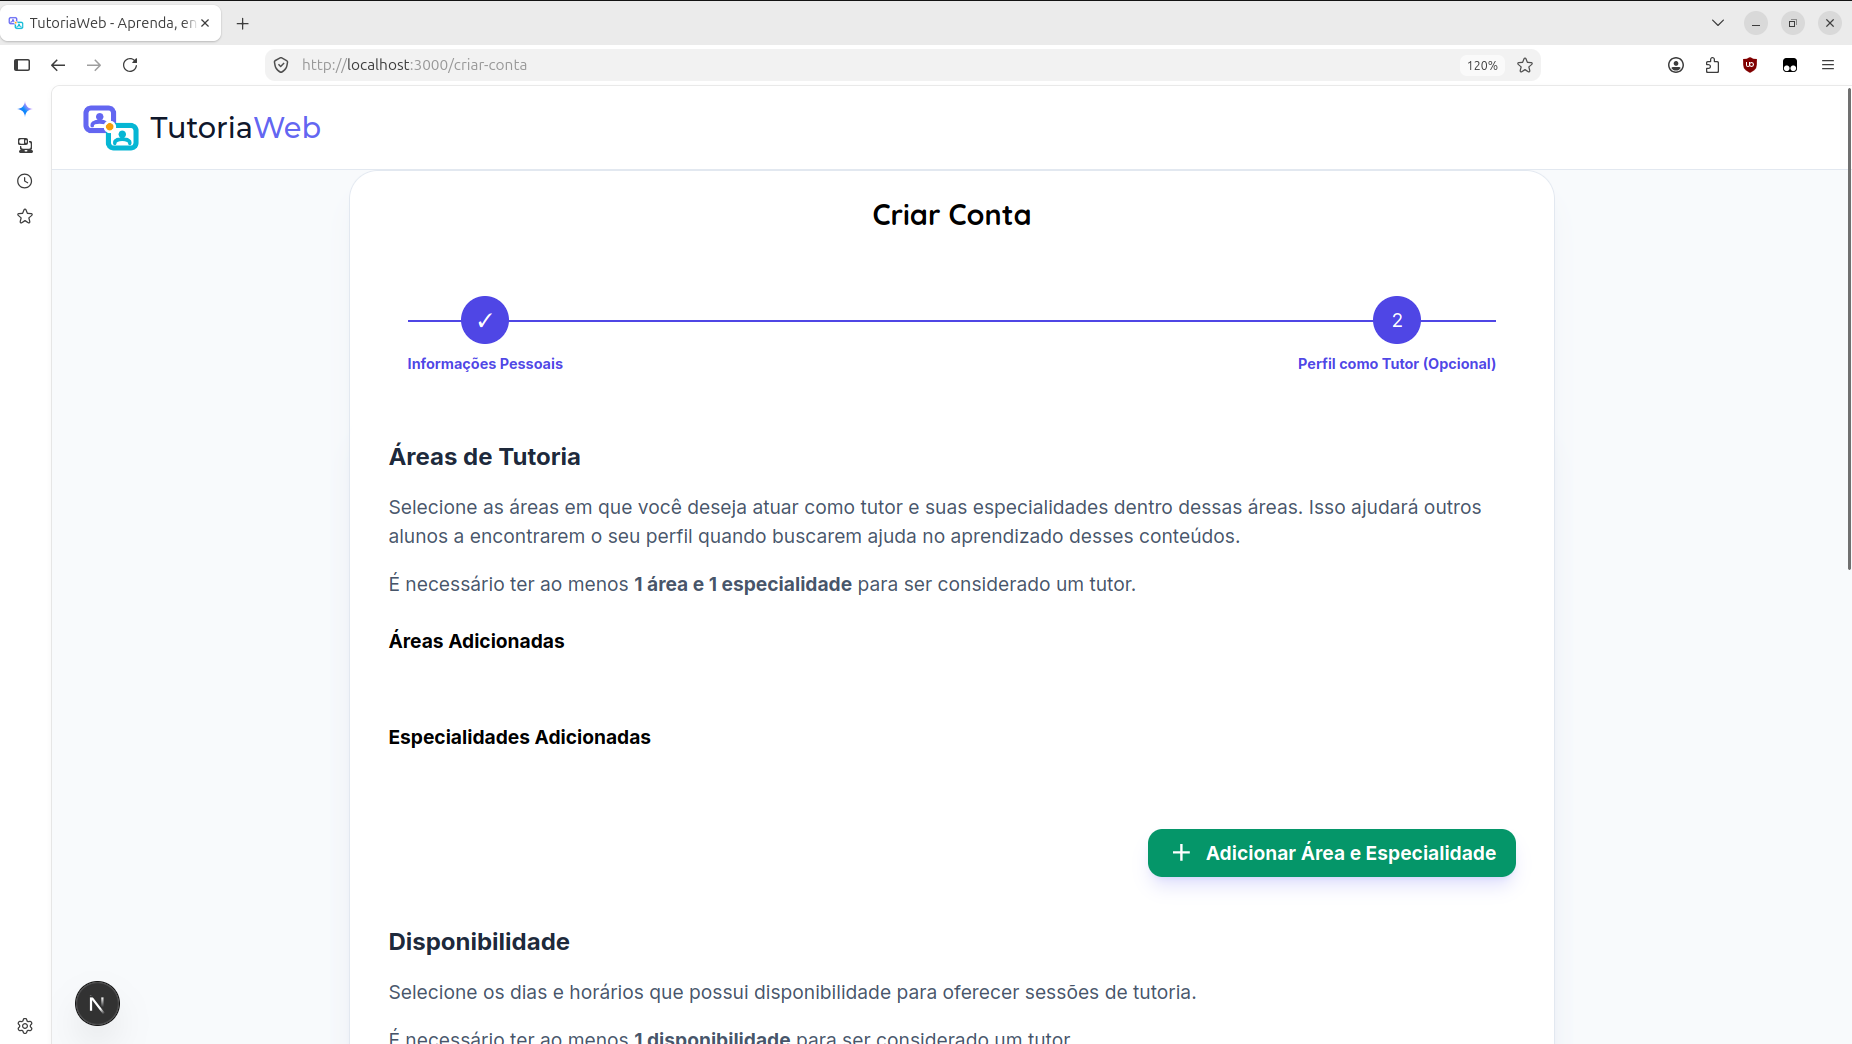
\includegraphics[width=1.9\textwidth, height=0.90\textheight, keepaspectratio]{figuras/criarConta2.png}
    
    
        Fonte: Autoria própria.
        
        \vspace{0.2cm}
            
        \label{fig:criarConta2}
    \end{figure}
\end{landscape}
\clearpage

\clearpage

\begin{landscape}
    \setlength{\oddsidemargin}{\evensidemargin}
    \numeracaoPaisagem
    \begin{figure}[H]
        \centering
        \caption{\textit{Modal} de cadastro de área e especialidade.} 
        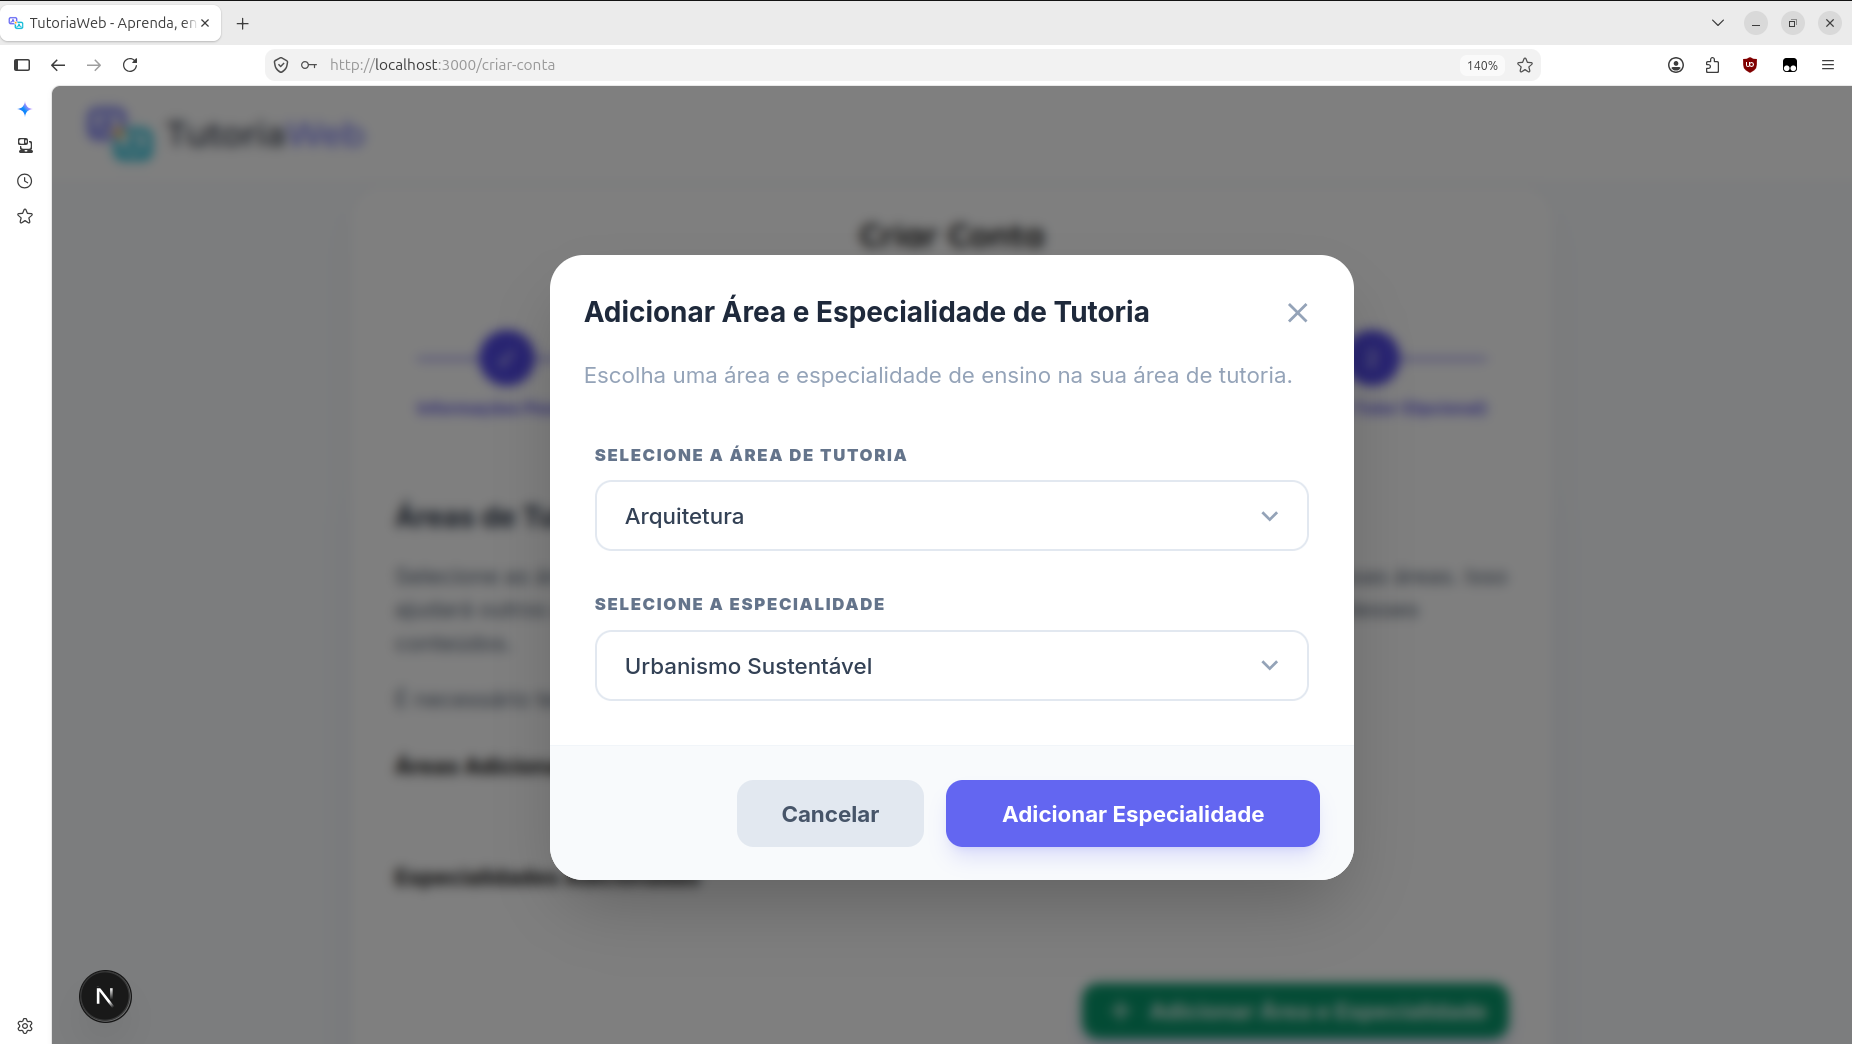
\includegraphics[width=1.9\textwidth, height=0.90\textheight, keepaspectratio]{figuras/modalArea.png}
    
    
        Fonte: Autoria própria.
        
        \vspace{0.2cm}
            
        \label{fig:modalArea}
    \end{figure}
\end{landscape}

\clearpage

\begin{landscape}
    \setlength{\oddsidemargin}{\evensidemargin}
    \numeracaoPaisagem
    \begin{figure}[H]
        \centering
        \caption{\textit{Modal} de cadastro de disponibilidade.} 
        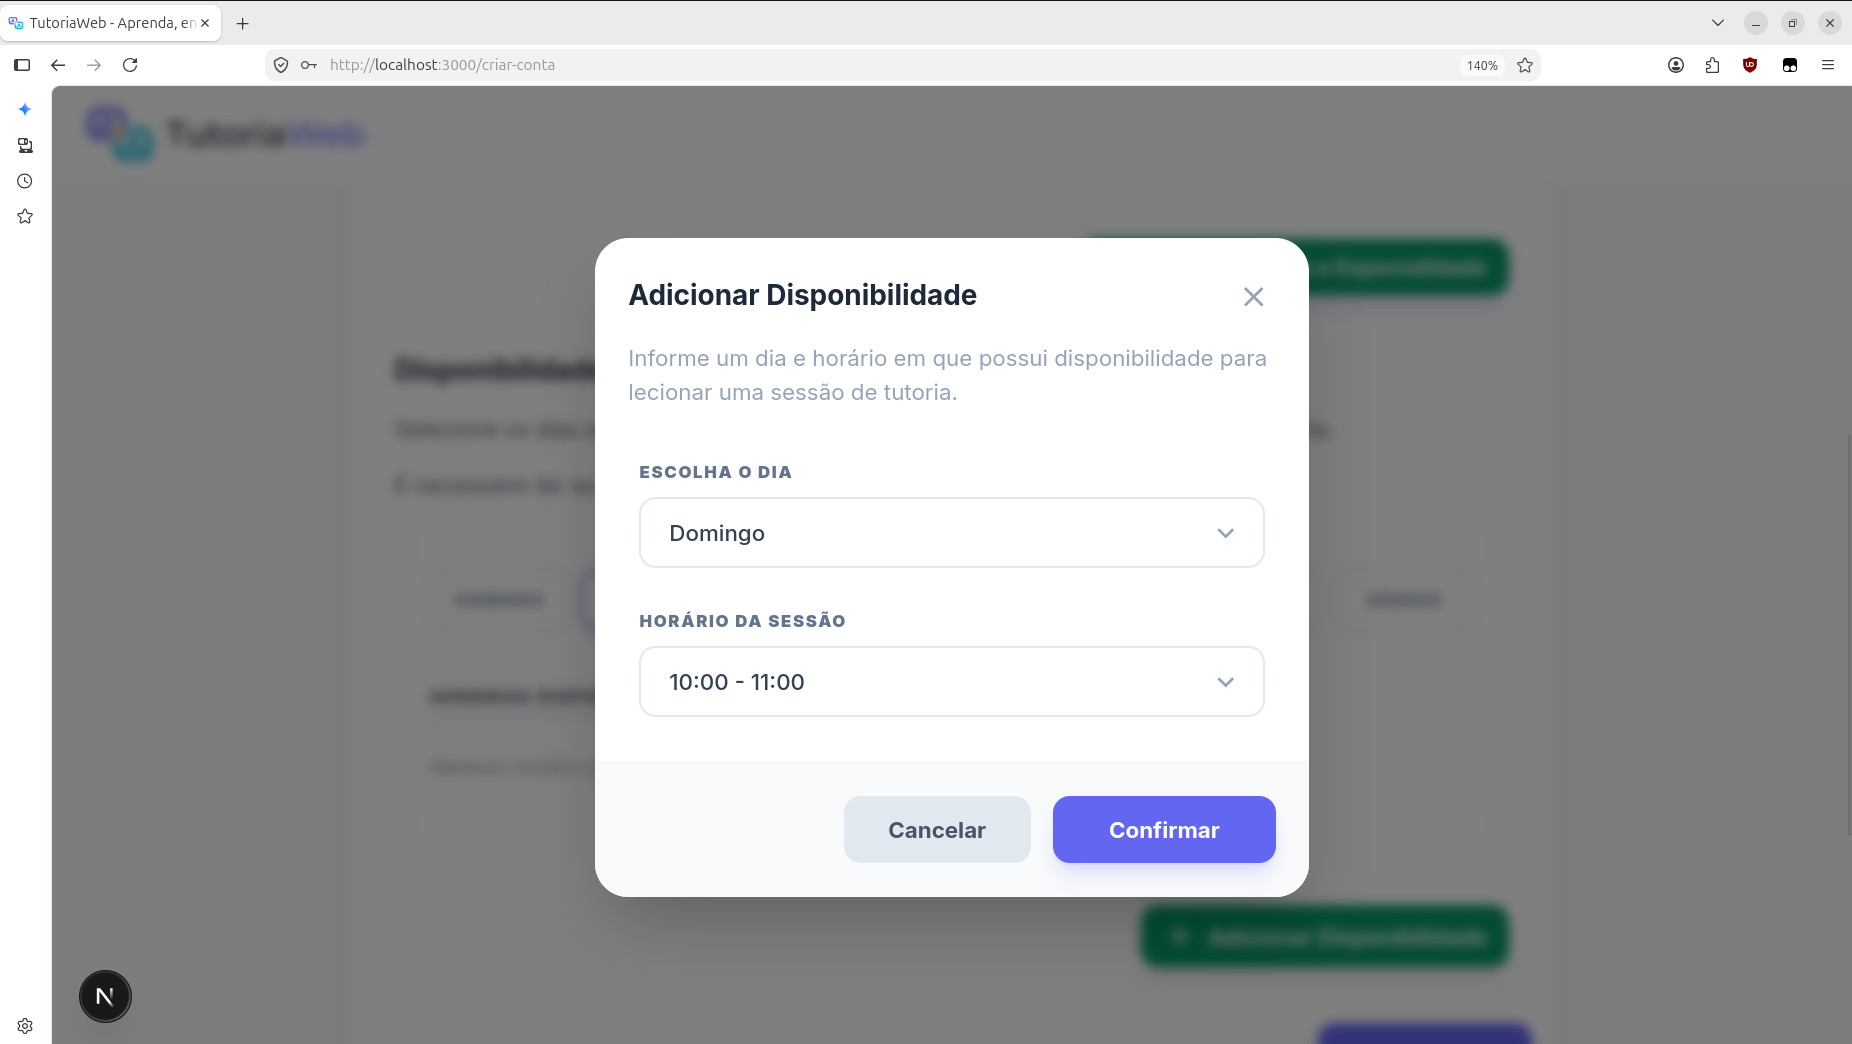
\includegraphics[width=1.9\textwidth, height=0.90\textheight, keepaspectratio]{figuras/modalAgenda.png}
    
    
        Fonte: Autoria própria.
        
        \vspace{0.2cm}
            
        \label{fig:modalAgenda}
    \end{figure}
\end{landscape}
\clearpage

Dois campos obrigatórios para preenchimento são Estado e Cidade. Para se obter a lista de estados e cidades do Brasil, foram utilizadas APIs do IBGE (Instituto Brasileiro de Geografia e Estatística). Antes da página ser exibida ao usuário, é feita uma requisição à API de estados para carregamento dos dados no campo de seleção do formulário. Quando o usuário seleciona uma cidade, a requisição à API de cidades acontece, sendo usado um filtro para carregar apenas as cidades do estado selecionado.

Durante o processo de desenvolvimento da criação de conta, foram descobertas as bibliotecas React Hook Form e Zod. React Hook Form é uma biblioteca para React utilizada para formulários em que um dos principais benefícios é reduzir o número de re-renderizações da tela causados pelo preenchimento dos campos, além dos campos serem carregados na tela mais rapidamente \cite{rhf2026}. Zod é uma biblioteca para React de validações com TypeScript que possibilita criar estruturas de dados para se realizar validações \cite{zod}. Ambas podem ser usadas em conjunto, com o Zod contendo uma estrutura para validar os campos do formulário.

Antes dessa descoberta, os formulários estavam sendo criados com o \textit{hook} \textit{useState} do React, que segundo \citeonline{reactUseState}, é usado para gerenciar valores, permitindo a consulta e alteração deles, e re-renderizando o componente para exibir o novo valor para o usuário. O problema é a re-renderização: a cada vez que um campo de formulário possui seu valor alterado, toda a tela é renderizada novamente. Isso prejudica a performance para o usuário, especialmente em inputs de texto, onde o valor do campo é alterado diversas vezes devido às digitações.

Em adição a isso, as validações estavam sendo realizadas com HTML puro, funções de detecção de mudanças do React e uso de condicionais. Diante desses fatores, utilizar as bibliotecas citadas se mostrou uma oportunidade de otimização, melhorando a performance da aplicação e aumentando a manutenibilidade do código, visto que as validações do Zod são mais fáceis de se fazer. Os formulários desenvolvidos até então foram refatorados para usá-las e os formulários novos foram criados utilizando-as.

Durante o desenvolvimento dessa US, os autores tiveram a ideia de adicionar um campo denominado ``Sobre mim'', cuja finalidade é permitir que o usuário insira um texto descritivo sobre si mesmo, que é exibido em sua página de perfil. Para que isso fosse possível, o atributo ``sobremim'' foi adicionado na tabela ``USUARIO'' no banco de dados, com limite de até 500 caracteres.

O desenvolvimento do \textit{backend} enfrentou desafios técnicos relevantes. Inicialmente, o uso do \textit{framework} Django exigiu adaptações arquiteturais, visto que seu comportamento padrão atribui identificadores numéricos automáticos a todas as entidades.
Além disso, a adoção da classe abstrata de usuário (\textit{AbstractUser}) demandou cuidado extra para assegurar a manutenção e compatibilidade dos atributos e relacionamentos nativos do DRF.

No que tange à infraestrutura, a conteinerização via Docker revelou conflitos estruturais entre a modelagem de dados planejada para o MySQL e as tabelas geradas de forma automatizada pelas migrações do ORM do Django. Por fim observou-se um problema de sincronismo durante a inicialização dos contêineres: o tempo necessário para o MySQL ficar pronto para aceitar conexões causava falhas na inicialização da aplicação, que tentava se comunicar com uma porta de banco de dados ainda indisponível. Isso foi resolvido com um \textit{script} que verifica se o MySQL já esta sendo executado na porta de rede declarada.

Outra alteração arquitetural significativa ocorreu no gerenciamento de arquivos. A concepção original estipulava a alocação das imagens em serviços externos, mantendo-se apenas a URL de acesso na base de dados relacional. Visaando maior centralização, essa estratégia foi substituída pela adoção de um \textit{data lake} referenciado diretamente pelo \textit{backend}, estruturado de modo a utilizar o endereço de e-mail do usuário como identificador único para o armazenamento de foto de perfil.

O desenvolvimento do \textit{frontend} passou por dois grandes problemas. O primeiro deles foi a falta de componentes reutilizáveis. Muitos elementos visuais que compõem a página não haviam sido criados até então, como \textit{modais}, sendo apenas possível aproveitar o conjunto de \textit{label} e \textit{input}, que já haviam sido criados na US01.

O segundo problema é a complexidade da página. Embora simples visualmente, ela é composta por muitos elementos visuais e regras de validação, que consumiram tempo considerável para serem criados. 

\subsubsection[US02: Recuperar Senha]{US02: Recuperar Senha}

A estimativa inicial para o desenvolvimento da US02 era na Semana 1, em conjunto com a US01, de 08 a 14 de março. O \textit{backend} foi desenvolvido entre 08 e 18 de março simultaneamente com a US01. O \textit{frontend} da página foi desenvolvido em 14 de março, sendo a integração com o \textit{backend} feita em 22 de março e no dia 27 de março sendo feita uma refatoração para utilização das bibliotecas React Hook Form e Zod no formulário.

Durante o desenvolvimento da funcionalidade, outra biblioteca foi adicionada na aplicação: Material UI. Conforme \cite{materialUI}, o Material UI é uma biblioteca React que oferece componentes de elementos visuais prontos para uso e com opções de customização.

Essa adição foi feita para atender ao CA04: exibir uma mensagem na tela após o usuário solicitar a recuperação de senha. Para isso, foi utilizado o componente \textit{Snackbar}, que trata-se de uma notificação visual que surge na tela exibindo uma mensagem, permitindo customização do texto que é exibido e também da cor da notificação. Essa biblioteca foi utilizada em outras funcionalidades da aplicação para informar o usuário sobre o resultado de uma ação, sendo a notificação exibida diferentes cores, como verde para sucesso e vermelho para erro.

A página pode ser observada na Figura \ref{fig:telaRecuperarSenha}. A notificação de sucesso, exibida após o usuário realizar o pedido de recuperação e ser redirecionado para a página de \textit{login}, pode ser observada na Figura \ref{fig:telaRecuperarSenhaErro}. A notificação de erro, caso a requisição seja feita mas não exista conexão com o servidor do \textit{backend}, pode ser observada na Figura \ref{fig:telaRecuperarSenhaSucesso}.

\clearpage

\begin{landscape}
    \setlength{\oddsidemargin}{\evensidemargin}
    \numeracaoPaisagem
    \begin{figure}[H]
        \centering
        \caption{Página de recuperação de senha.} 
        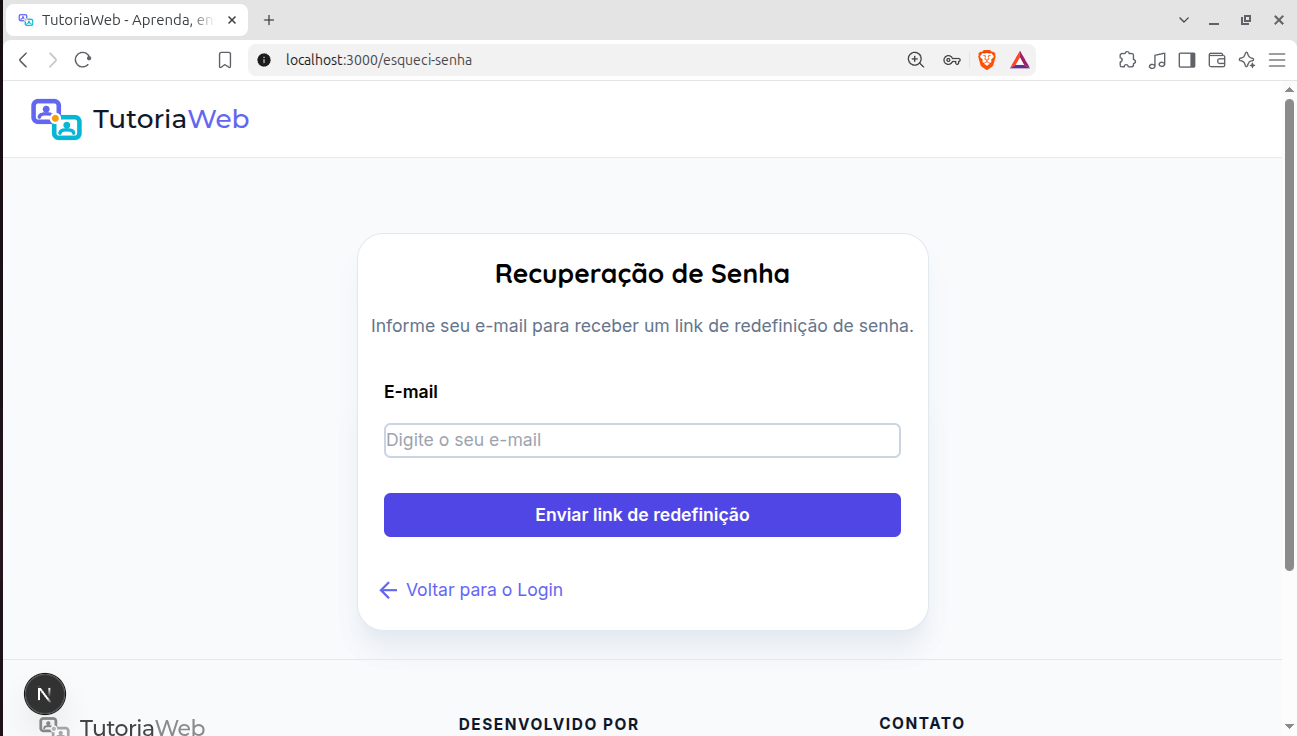
\includegraphics[width=1.9\textwidth, height=0.90\textheight, keepaspectratio]{figuras/telaRecuperarSenha.png}
    
    
        Fonte: Autoria própria.
        
        \vspace{0.2cm}
            
        \label{fig:telaRecuperarSenha}
    \end{figure}
\end{landscape}

\clearpage

\begin{landscape}
    \setlength{\oddsidemargin}{\evensidemargin}
    \numeracaoPaisagem
    \begin{figure}[H]
        \centering
        \caption{Notificação de erro na tentativa de requisição.} 
        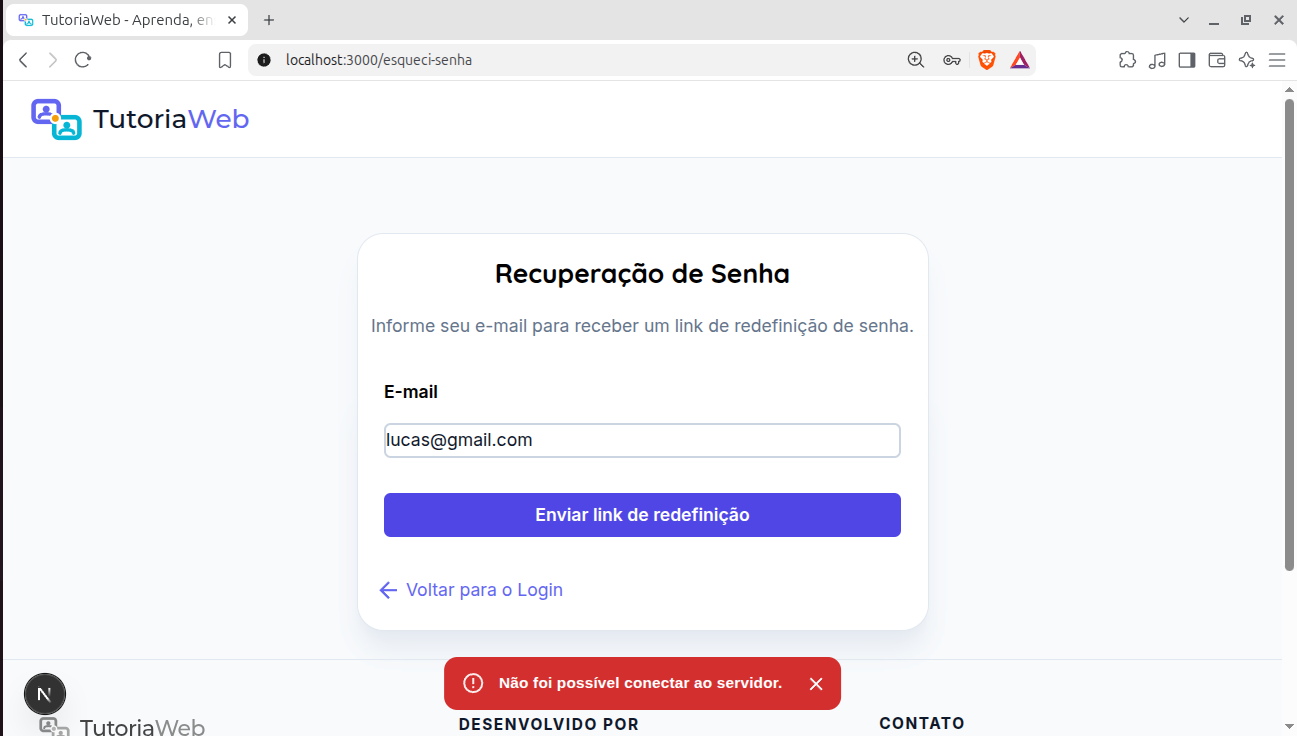
\includegraphics[width=1.9\textwidth, height=0.90\textheight, keepaspectratio]{figuras/telaRecuperarSenhaErro.png}
    
    
        Fonte: Autoria própria.
        
        \vspace{0.2cm}
            
        \label{fig:telaRecuperarSenhaErro}
    \end{figure}
\end{landscape}
\clearpage

\clearpage

\begin{landscape}
    \setlength{\oddsidemargin}{\evensidemargin}
    \numeracaoPaisagem
    \begin{figure}[H]
        \centering
        \caption{Notificação de sucesso após redirecionamento para \textit{login}.} 
        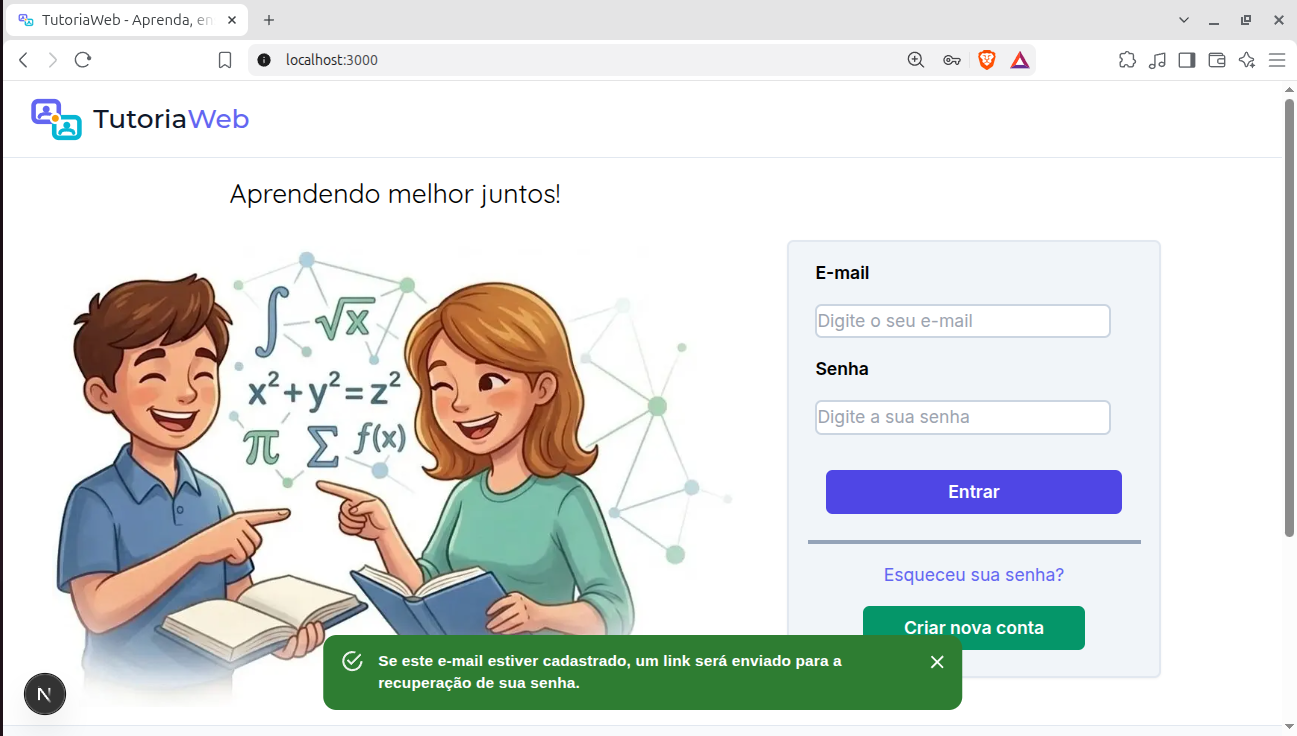
\includegraphics[width=1.9\textwidth, height=0.90\textheight, keepaspectratio]{figuras/telaRecuperarSenhaSucesso.png}
    
    
        Fonte: Autoria própria.
        
        \vspace{0.2cm}
            
        \label{fig:telaRecuperarSenhaSucesso}
    \end{figure}
\end{landscape}
\clearpage

A página consiste de um card informativo com um campo de formulário para um e-mail ser inserido e um botão para submissão. Independente do e-mail de fato estar registrado como pertencente a um usuário, ocorre o mencionado redirecionamento para a página de \textit{login} e a exibição da notificação. No caso do registo de fato existir, um e-mail é enviado pelo \textit{backend}, contendo um \textit{link} que, quando clicado, leva para a página de alteração de senha. O e-mail enviado pode ser observado na Figura \ref{fig:emailRecuperacaoSenha}.

\begin{landscape}
    \setlength{\oddsidemargin}{\evensidemargin}
    \numeracaoPaisagem
    \begin{figure}[H]
        \centering
        \caption{E-mail com link para alteração de senha.} 
        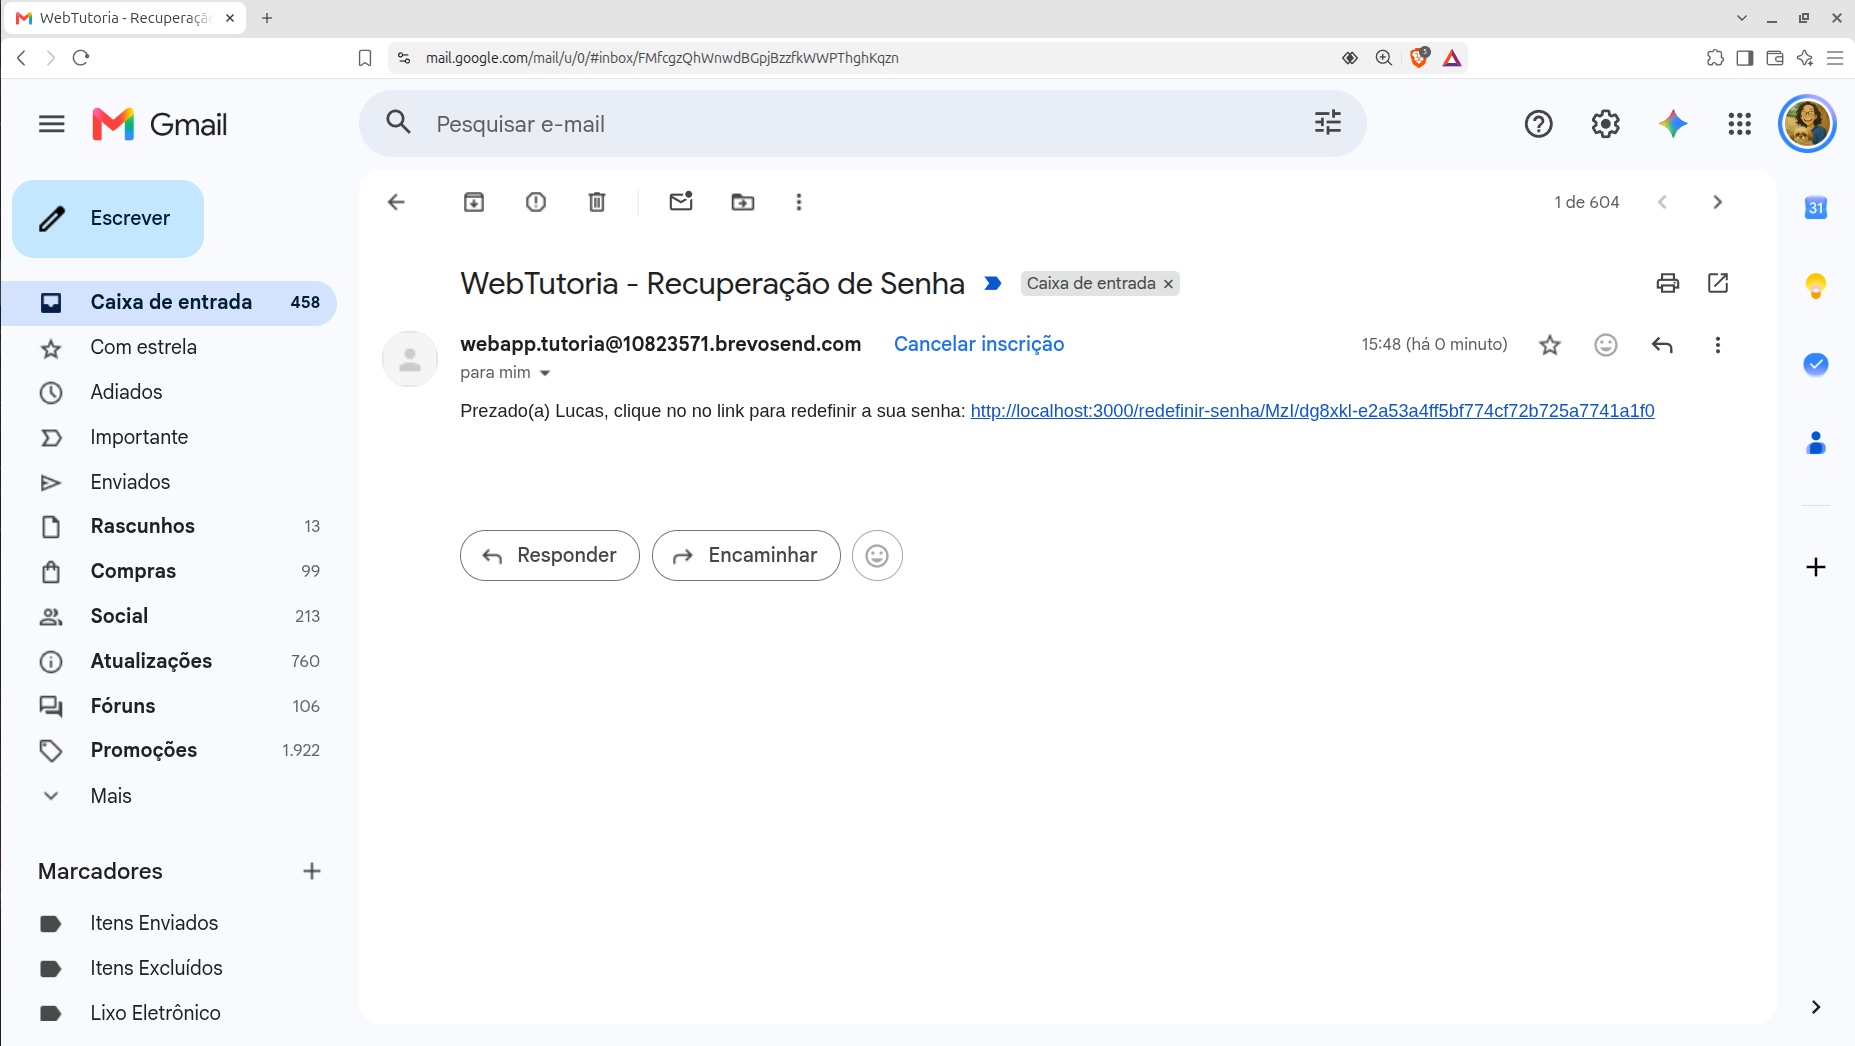
\includegraphics[width=1.9\textwidth, height=0.90\textheight, keepaspectratio]{figuras/emailRecuperacaoSenha.png}
    
    
        Fonte: Autoria própria.
        
        \vspace{0.2cm}
            
        \label{fig:emailRecuperacaoSenha}
    \end{figure}
\end{landscape}
\clearpage

No desenvolvimento do \textit{backend}, um dos desafios encontrados foi garantir que o \textit{token} de recuperação de senha fosse de uso único. Após pesquisas na documentação do \textit{framework}, constatou-se que a função \textit{default\_token\_generator} utiliza o campo \textit{last\_update} como um dos parâmetros para a geração de seu \textit{hash}. Consequentemente, ao validar a requisição, a aplicação força a atualização desse campo, o que altera os parâmetros base da criptografia e invalida automaticamente o \textit{token} recém-utilizado, impedindo acessos subsequentes.

Outro obstáculo enfrentado no desenvolvimento foi a seleção de um serviço de envio de e-mails gratuito que atendesse ao CA03 da US02. Após pesquisa por soluções viáveis, a plataforma Brevo foi adotada para viabilizar essa comunicação sem gerar custos ao projeto.

Não houve nenhuma dificuldade no desenvolvimento do \textit{frontend}.

\subsubsection[US03: Alterar Senha]{US03: Alterar Senha}

A estimativa inicial para o desenvolvimento da US03 era na Semana 2, de 15 a 21 de março. O \textit{backend} foi desenvolvido junto a US02 e finalizado no dia 18 de março. O \textit{frontend} foi desenvolvido em grande parte no dia 16 de março, com uma refatoração para uso do React Hook Form e Zod e a integração com o \textit{backend} sendo feitas no dia 25 de março.

A página de alteração de senha é uma página com rotas dinâmicas, recebendo dois parâmetros em sua URL: o UID (\textit{User ID}), que é um número identificador do registro do usuário no banco, mas transfigurado, e um \textit{token}, ambos provenientes do \textit{link} enviado por e-mail após o pedido de recuperação de senha ser feito.

Devido à forma com que rotas dinâmicas é feita no Next.js, onde apenas é informado a quantidade e nome dos parâmetros com compõem a URL, a página pode ser acessada colocando dois valores quaisquer na URL. Entretanto, o \textit{backend} valida o UID e o \textit{token} na requisição de alteração de senha. Caso algum deles seja inválido, é retornada uma mensagem de erro, que é exibida por uma \textit{Snackbar} na tela.

A página em si consiste de um formulário de dois campos, onde a nova senha deve ser inserida duas vezes. A senha deve atender aos critérios de possuir mais de 10 caracteres, possui um número e possuir um caractere especial. Essas exigências possuem a finalidade de fazer o usuário criar uma senha mais complexa, de forma a evitar ataques maliciosos à sua conta. Os critérios são usados tanto na alteração quanto na criação da senha na página de criação de conta. São exibidas mensagens de erro em casos de senhas inválidas ou desiguais.

Caso a requisição seja bem-sucedida, é exibida uma notificação informativa para o usuário e é feito um redirecionamento para a tela de \textit{login}. A página pode ser observada na Figura \ref{fig:paginaRedefinicaoSenha}.

Durante o desenvolvimento da US04, os autores pensaram em ser uma boa ideia se um usuário já conectado à aplicação pudesse alterar a senha de sua conta através da edição de perfil. Sendo assim, essa funcionalidade foi também implementada nessa página. Clicando no botão ``Alterar Senha'', é exibida uma \textit{modal} na tela para essa finalidade. Essa \textit{modal} utiliza uma requisição diferente no \textit{backend}, e exige que o usuário informe sua senha atual e a senha nova, sendo usado um novo critério de validação, que é a senha atual informada no campo ser de fato a senha do usuário. Essa \textit{modal} pode se vista na Figura \ref{fig:modalAlteracaoSenha}.

Não houveram dificuldades no desenvolvimento do \textit{backend} e \textit{frontend} dessa US.

\begin{landscape}
    \setlength{\oddsidemargin}{\evensidemargin}
    \numeracaoPaisagem
    \begin{figure}[H]
        \centering
        \caption{Página de alteração de senha.} 
        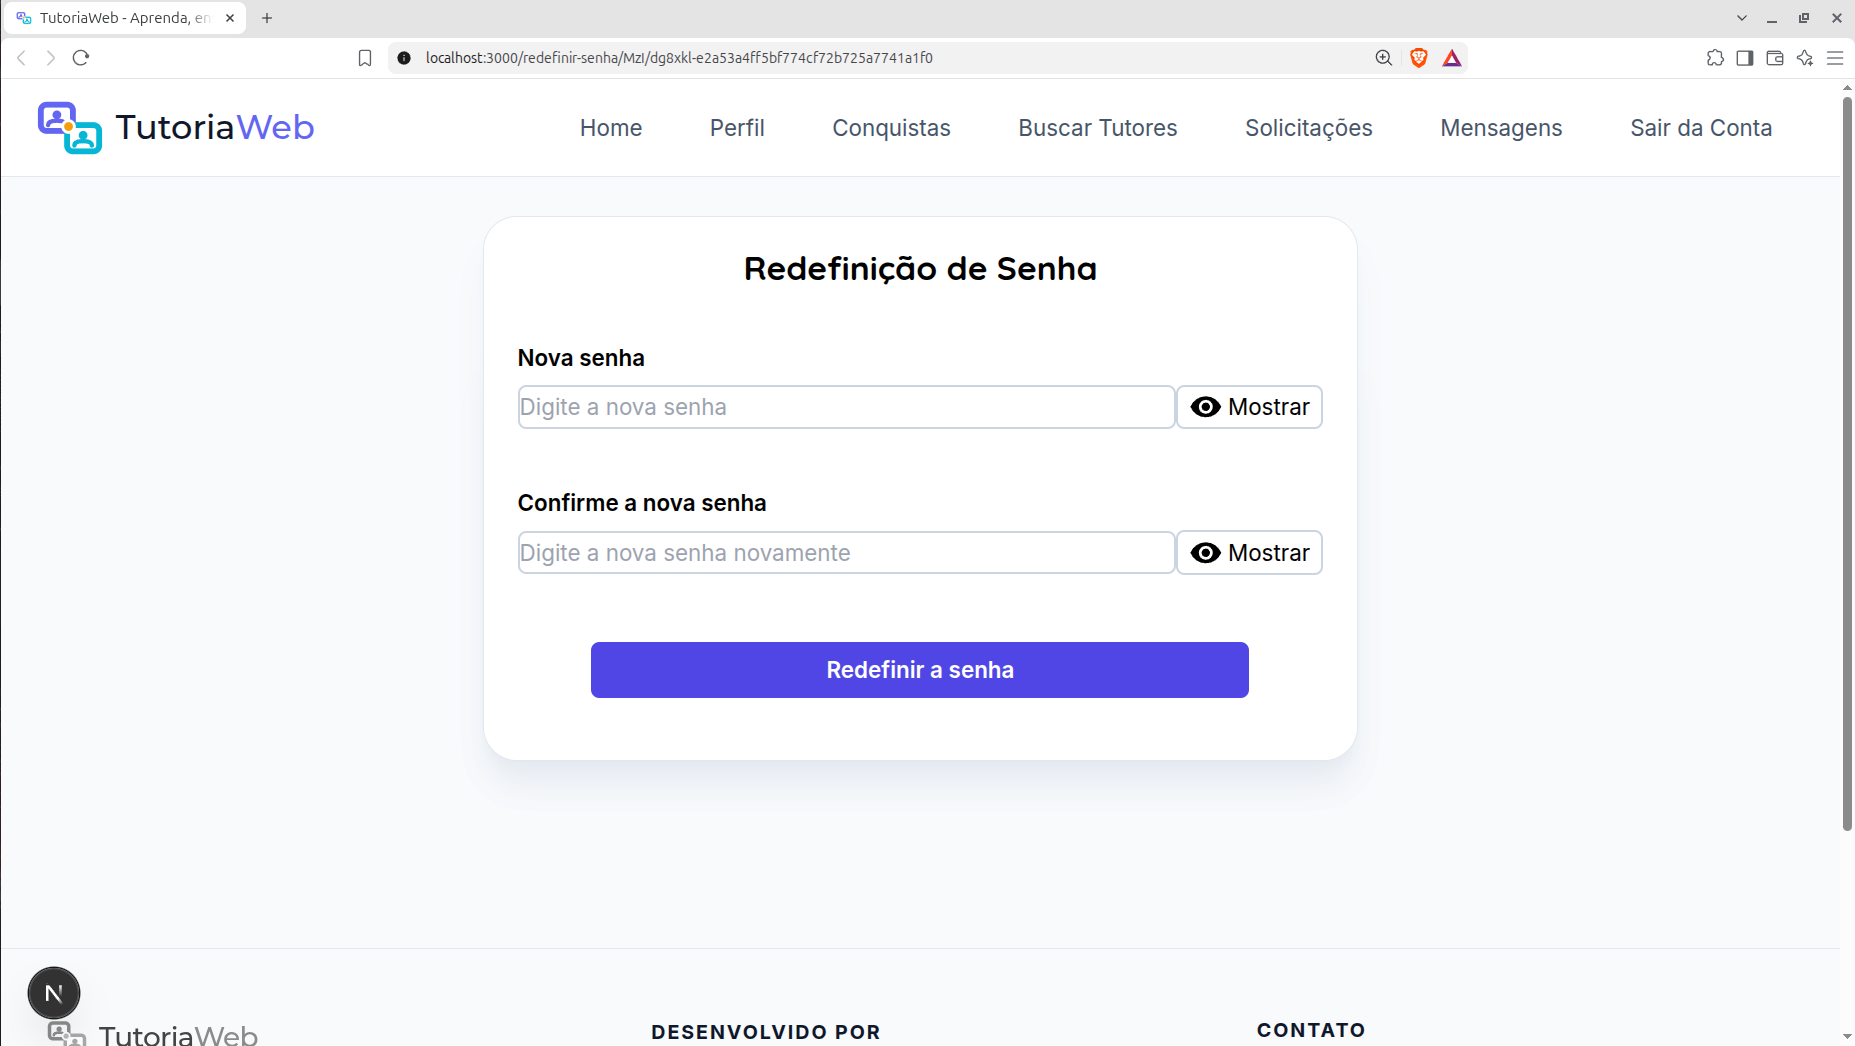
\includegraphics[width=1.9\textwidth, height=0.90\textheight, keepaspectratio]{figuras/paginaRedefinicaoSenha.png}
    
    
        Fonte: Autoria própria.
        
        \vspace{0.2cm}
            
        \label{fig:paginaRedefinicaoSenha}
    \end{figure}
\end{landscape}
\clearpage

\begin{landscape}
    \setlength{\oddsidemargin}{\evensidemargin}
    \numeracaoPaisagem
    \begin{figure}[H]
        \centering
        \caption{\textit{Modal} de alteração de senha.} 
        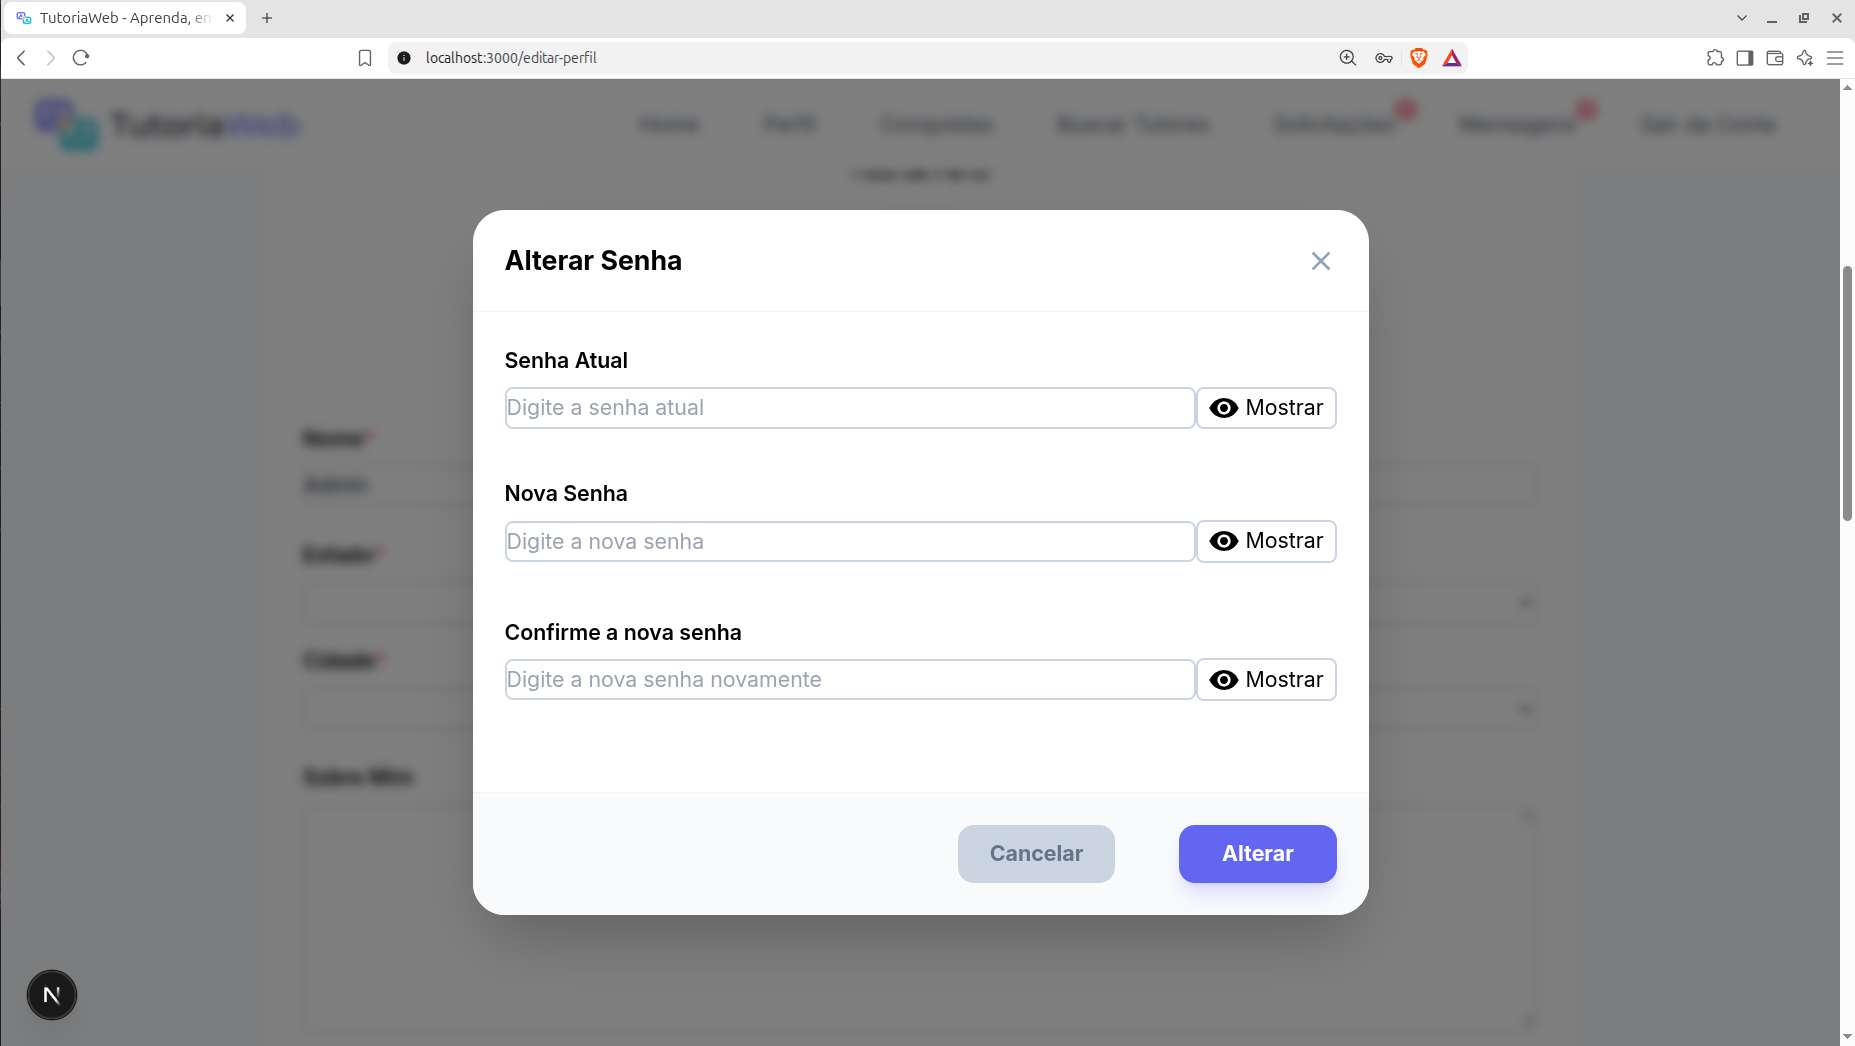
\includegraphics[width=1.9\textwidth, height=0.90\textheight, keepaspectratio]{figuras/modalAlteracaoSenha.png}
    
    
        Fonte: Autoria própria.
        
        \vspace{0.2cm}
            
        \label{fig:modalAlteracaoSenha}
    \end{figure}
\end{landscape}
\clearpage

\subsection[Funcionalidade 2: Gerenciamento de Perfil]{Funcionalidade 2: Gerenciamento de Perfil}

\subsubsection[US04: Alterar Informações]{US04: Alterar Informações}
\label{sec:us04}

A estimativa inicial para o desenvolvimento dessa US era na Semana 2, de 15 a 21 de março, juntamente com a US03. O \textit{backend} atrasou o desenvolvimento em uma semana, começando no dia 23 de março e finalizando no dia 27 de março, enquanto que o \textit{frontend} começou a ser desenvolvido em 2 de abril e finalizou em 30 de abril.

O atraso para o começo do desenvolvimento do \textit{backend} foi ocasionada pela mudança arquitetural do perfil de usuário descritas na Subseção \ref{sec:us20}.

O atraso do \textit{frontend} se deve em grande parte por refatorações em páginas anteriores a fins de otimização e a implementação da página de criação de conta, que se tornou mais prioritária. O grande período de desenvolvimento se deve ao fato dessa US ter exigido a criação de duas páginas: a página de perfil e a página de edição de perfil. Uma vez que a página de perfil estava finalizada, grande parte do código pode ser aproveitado para o desenvolvimento da segunda página, acelerando sua finalização. A página de perfil e a área da página de edição de perfil pertinente a essa US podem ser vistas nas Figuras \ref{fig:telaPerfil1}, \ref{fig:telaPerfil2}, \ref{fig:telaEditarPerfil1} e \ref{fig:telaEditarPerfil2}.

Antes da página ser apresentada ao usuário, é feita uma requisição ao \textit{backend} para se obter as informações do perfil do usuário, sendo utilizado um ícone giratório (\textit{spinner}) para indicar carregamento de dados. Esse \textit{feedback} visual também foi utilizado em todas as outras páginas que solicitam dados do \textit{backend} para exibição na tela, como a página de conquistas ou a página de perfil de outros usuários.

A página apresenta os campos preenchidos com os dados retornados pelo \textit{backend}, permitindo a alteração dos mesmos. Novamente, as APIs do IBGE são utilizadas para seleção de cidade e estado.

Durante o desenvolvimento do \textit{backend} ocorreu o contratempo de distinguir os dados retornados de um usuário autenticado na aplicação em relação aos dados expostos de usuários externos. Para solucionar tal desafio, foi necessário implementar \textit{Serializers} distintos para cada contexto de acesso. Essa separação de responsabilidades contribuiu para o padrão arquitetural e construção e escalabilidade da API para funcionalidades desenvolvidas posteriormente.

Houve uma dificuldade no desenvolvimento do \textit{frontend} dessa funcionalidade. O CA04 exige que as alterações sejam refletidas imediatamente no perfil do usuário. Entretanto, a foto de perfil não estava sendo alterada na página de perfil após sua substituição. Após investigação, foi descoberto que isso se devia ao fato do navegador fazer \textit{cache} da imagem. Como ambas as imagens estavam compartilhando o mesmo nome no \textit{data lake} e no dado retornado pela requisição do \textit{backend}, o navegador assumia que não havia alterações e não buscava a nova foto.

Para resolver isso foi utilizada a técnica \textit{Cache Busting}, que segundo \citeonline{cacheBusting}, trata-se de forçar o navegador a fazer o \textit{download} da última versão de um arquivo, ao invés de utilizar uma versão ultrapassada armazenada em \textit{cache}. Isso foi feito acrescentando o horário exato que a página é acessada à fonte da imagem no componente visual que exibe a foto de perfil, dessa maneira sempre alterando o nome e prevenindo o uso da versão em \textit{cache}.

\begin{landscape}
    \setlength{\oddsidemargin}{\evensidemargin}
    \numeracaoPaisagem
    \begin{figure}[H]
        \centering
        \caption{Página de perfil.} 
        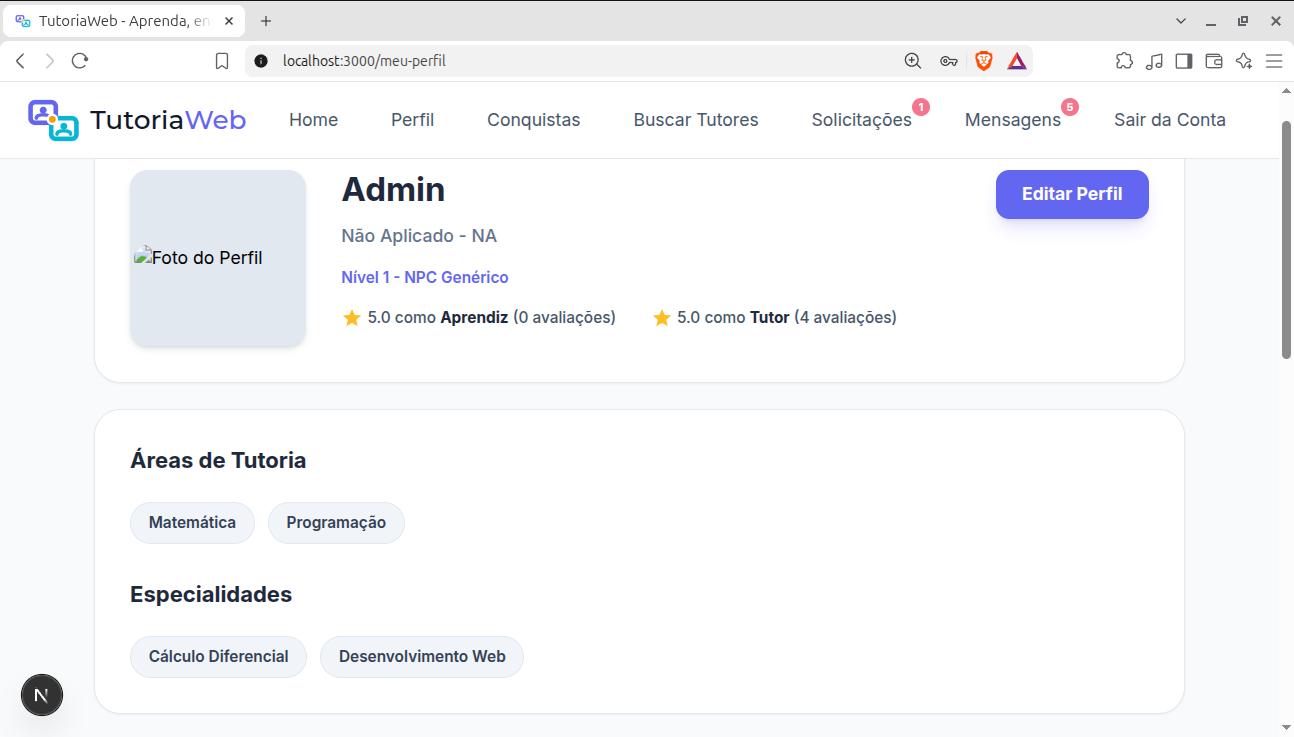
\includegraphics[width=1.9\textwidth, height=0.90\textheight, keepaspectratio]{figuras/telaPerfil1.png}
    
    
        Fonte: Autoria própria.
        
        \vspace{0.2cm}
            
        \label{fig:telaPerfil1}
    \end{figure}
\end{landscape}
\clearpage

\begin{landscape}
    \setlength{\oddsidemargin}{\evensidemargin}
    \numeracaoPaisagem
    \begin{figure}[H]
        \centering
        \caption{Continuação da página de perfil.} 
        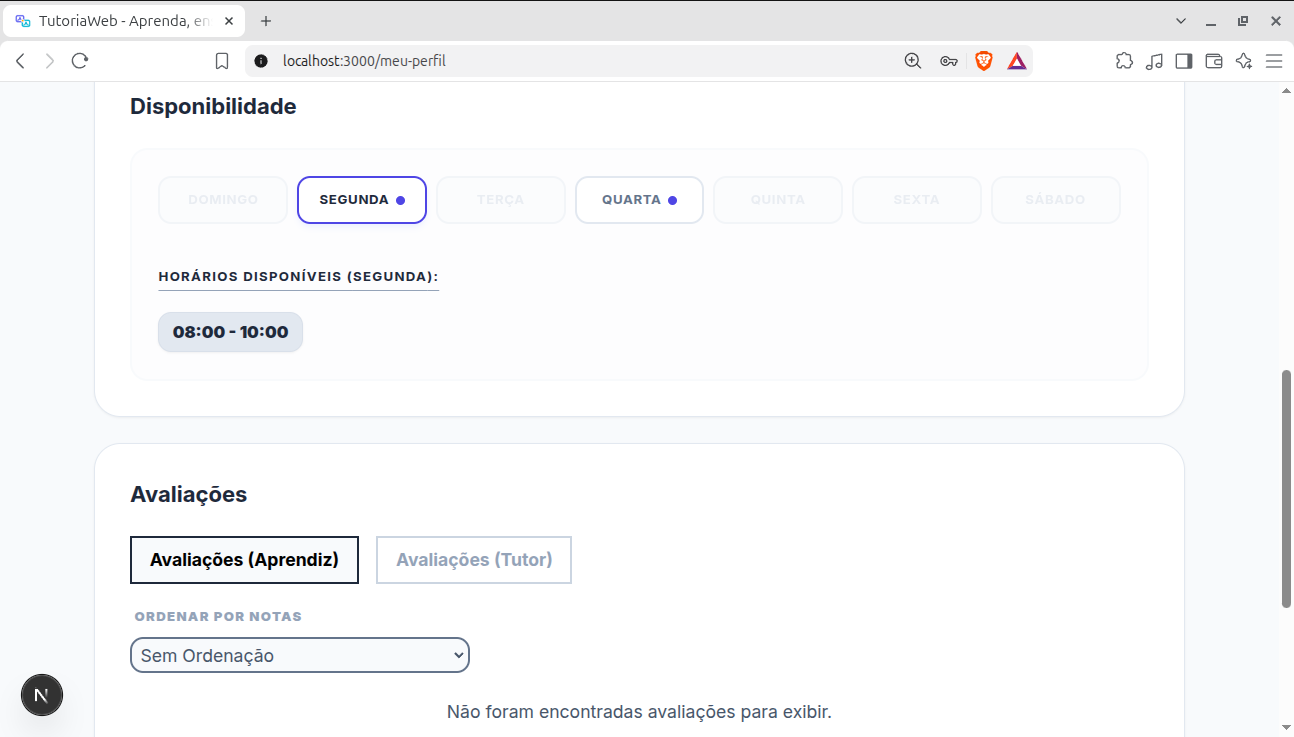
\includegraphics[width=1.9\textwidth, height=0.90\textheight, keepaspectratio]{figuras/telaPerfil2.png}
    
    
        Fonte: Autoria própria.
        
        \vspace{0.2cm}
            
        \label{fig:telaPerfil2}
    \end{figure}
\end{landscape}
\clearpage

\begin{landscape}
    \setlength{\oddsidemargin}{\evensidemargin}
    \numeracaoPaisagem
    \begin{figure}[H]
        \centering
        \caption{Página de edição de perfil.} 
        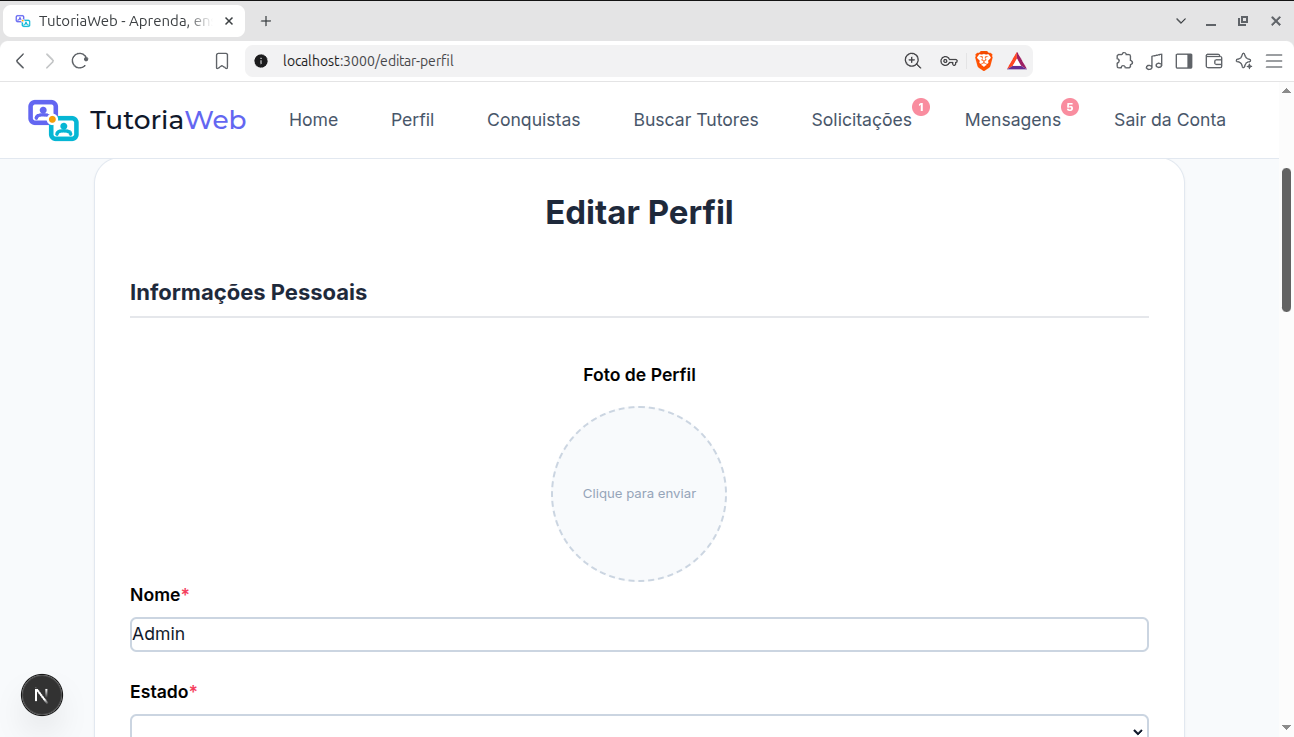
\includegraphics[width=1.9\textwidth, height=0.90\textheight, keepaspectratio]{figuras/telaEditarPerfil1.png}
    
    
        Fonte: Autoria própria.
        
        \vspace{0.2cm}
            
        \label{fig:telaEditarPerfil1}
    \end{figure}
\end{landscape}
\clearpage

\begin{landscape}
    \setlength{\oddsidemargin}{\evensidemargin}
    \numeracaoPaisagem
    \begin{figure}[H]
        \centering
        \caption{Continuação da página de edição de perfil} 
        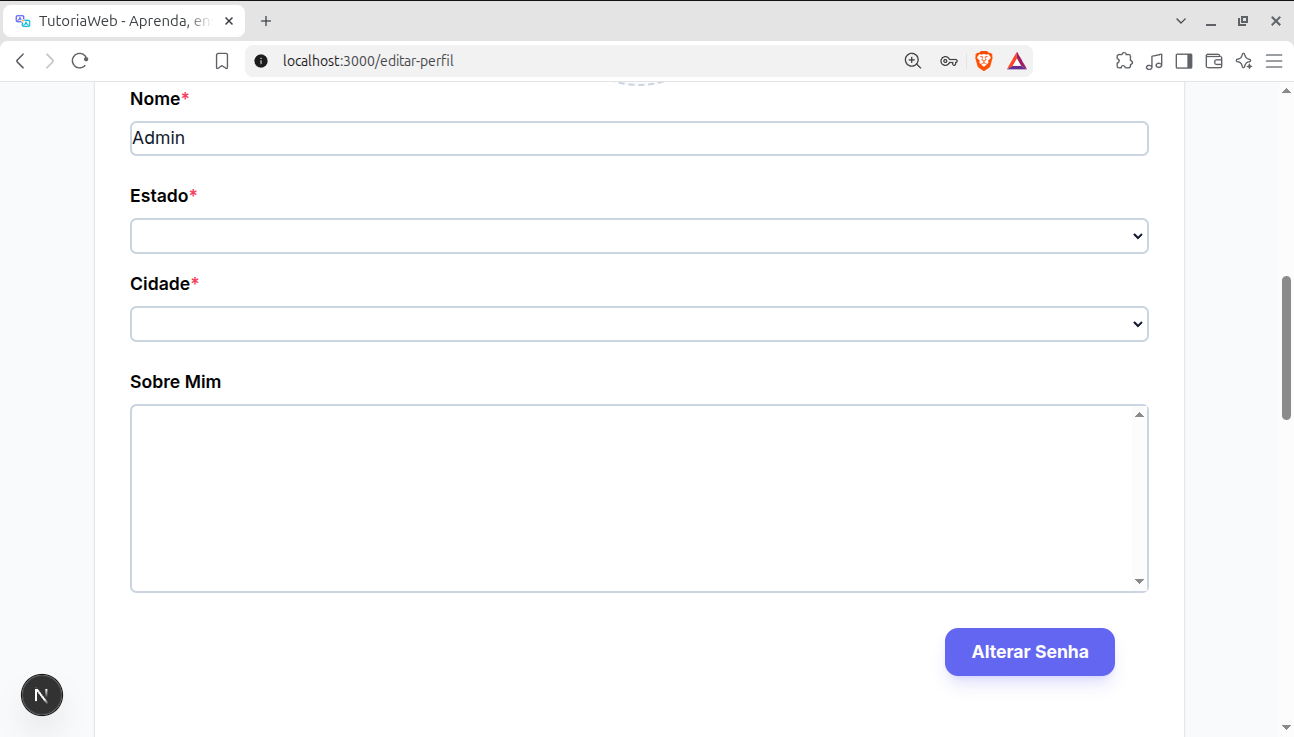
\includegraphics[width=1.9\textwidth, height=0.90\textheight, keepaspectratio]{figuras/telaEditarPerfil2.png}
    
    
        Fonte: Autoria própria.
        
        \vspace{0.2cm}
            
        \label{fig:telaEditarPerfil2}
    \end{figure}
\end{landscape}
\clearpage

\subsubsection[US05: Definir Agenda e US06: Gerenciar Especialidades]{US05: Definir Agenda e US06: Gerenciar Especialidades}
\label{sec:us05}

Essas US serão explicadas em uma subseção única por serem muito similares e simples, não havendo necessidade de uma subseção única para cada uma. A estimativa inicial para o desenvolvimento delas era na Semana 3, de 22 a 28 de março. O desenvolvimento do \textit{backend} iniciou-se somente em 27 de abril e encerrou-se no dia 02 de maio, sendo o atraso devido a demandas acumuladas do estágio e disciplinas de um dos autores. O desenvolvimento do \textit{frontend} dessas US começou em 16 de abril e foi pausado em 30 de abril, retomando em 11 de maio para integração dos \textit{endpoints} e finalizando em 15 de maio, sendo que durante esse período de pausa ocorreram o desenvolvimento do \textit{frontend} de outras US.

Essas funcionalidades são disponibilizadas ao usuário na página de edição de perfil, onde existe uma seção dedicada para elas. Essa seção pode ser observada nas Figuras \ref{fig:editarAreas} e \ref{fig:areaDisponibilidade}.

As áreas e especialidades de tutoria do usuário são listadas, bem como suas disponibilidades, organizadas em dias da semana e os horários disponíveis neles. Ao lado de cada um desses itens existe o ícone de uma lixeira, que quando clicado, abre uma \textit{modal} que permite ao usuário excluí-lo de seu perfil. Como exemplo, a \textit{modal} de deleção de disponibilidade pode ser observada na Figura \ref{fig:modalApagarDisponibilidade}.

Ao clicar no botão ``Adicionar Área'', abre-se uma \textit{modal} de seleção tanto da área quanto da especialidade, sendo inseridos ambos no perfil. A inserção de disponibilidades através da mesma forma, utilizando uma \textit{modal} permitindo selecionar um dia e um intervalo de 1 hora, abrangendo todas as 24 horas de um dia. Ambas as \textit{modais} já foram apresentadas anteriormente nas Figuras \ref{fig:modalArea} e \ref{fig:modalAgenda} da Subseção \ref{sec:us20}.

Essas alterações, bem como as alterações em informações de perfil da US04, só são efetuadas se o usuário clica no botão ``Salvar'' na página. Quando isso é feito, é feita uma verificação nas mudanças feitas nas áreas de tutor.

Caso um usuário não possua nenhuma área, especialidade e disponibilidade, mas adicionou essas informações em seu perfil, ele é registrado como um tutor, e passa a ser visível para outros na página de busca e recomendação de tutores.

Se o usuário possuia áreas, especialidades e disponibilidades mas optou por apagar todas elas, ele não é mais visível nos resultados de pesquisa de tutores. Entretanto, continua registrado como tutor no banco de dados, a fim de se manter o histórico de sessões que outros aprendizes tiveram com ele. Destaca-se novamente que, para ser um tutor, um usuário deve possuir ao menos uma disponibilidade, uma área de conhecimento e uma especialidade.

\begin{landscape}
    \setlength{\oddsidemargin}{\evensidemargin}
    \numeracaoPaisagem
    \begin{figure}[H]
        \centering
        \caption{Seção de gerenciamento de áreas e especialidades.} 
        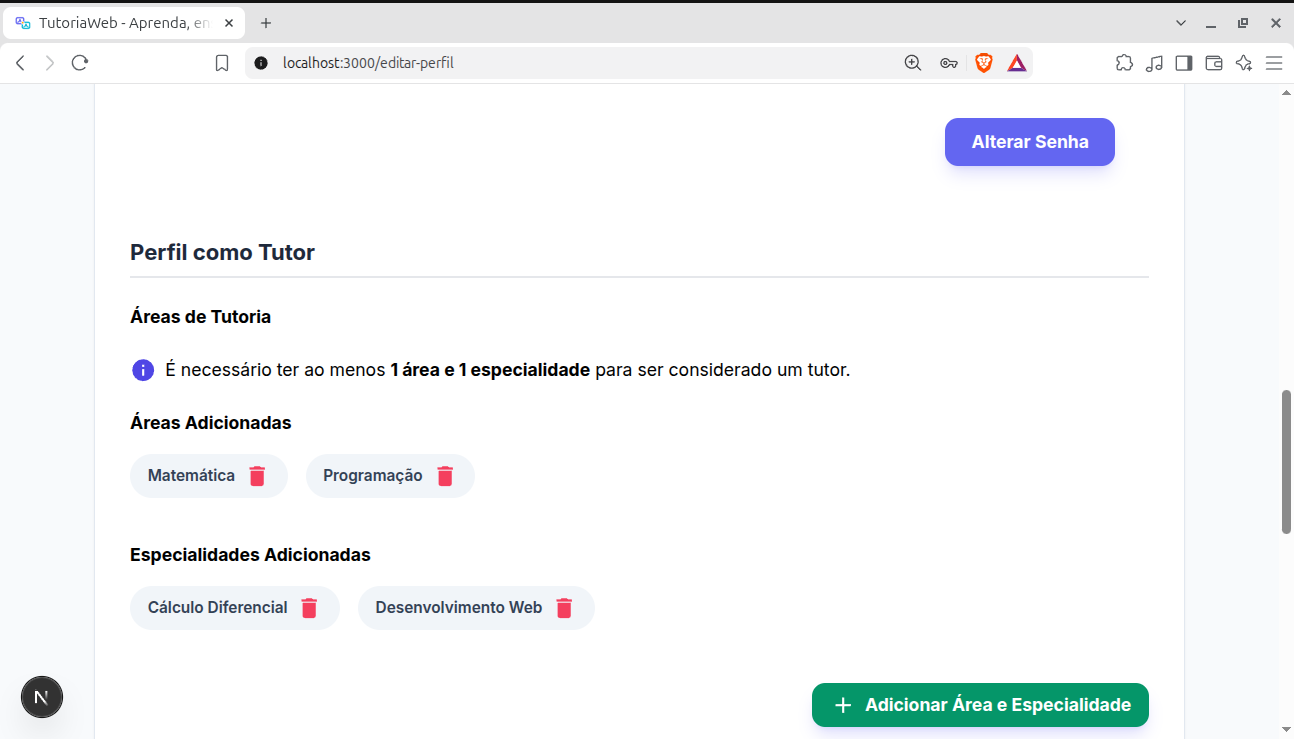
\includegraphics[width=1.9\textwidth, height=0.90\textheight, keepaspectratio]{figuras/editarAreas.png}
    
    
        Fonte: Autoria própria.
        
        \vspace{0.2cm}
            
        \label{fig:editarAreas}
    \end{figure}
\end{landscape}
\clearpage

\begin{landscape}
    \setlength{\oddsidemargin}{\evensidemargin}
    \numeracaoPaisagem
    \begin{figure}[H]
        \centering
        \caption{Seção de gerenciamento de disponibilidades.} 
        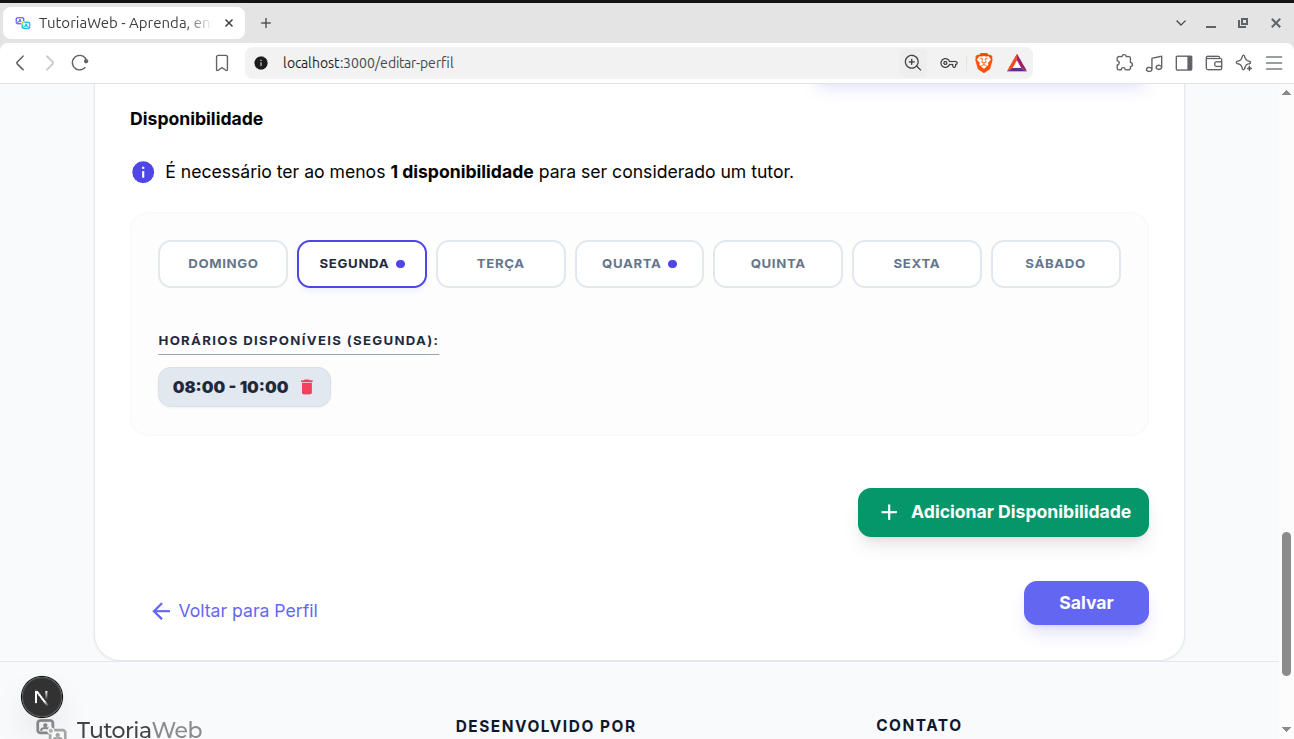
\includegraphics[width=1.9\textwidth, height=0.90\textheight, keepaspectratio]{figuras/areaDisponibilidade.png}
    
    
        Fonte: Autoria própria.
        
        \vspace{0.2cm}
            
        \label{fig:areaDisponibilidade}
    \end{figure}
\end{landscape}
\clearpage


\begin{landscape}
    \setlength{\oddsidemargin}{\evensidemargin}
    \numeracaoPaisagem
    \begin{figure}[H]
        \centering
        \caption{\textit{Modal} de deleção de disponibilidade.} 
        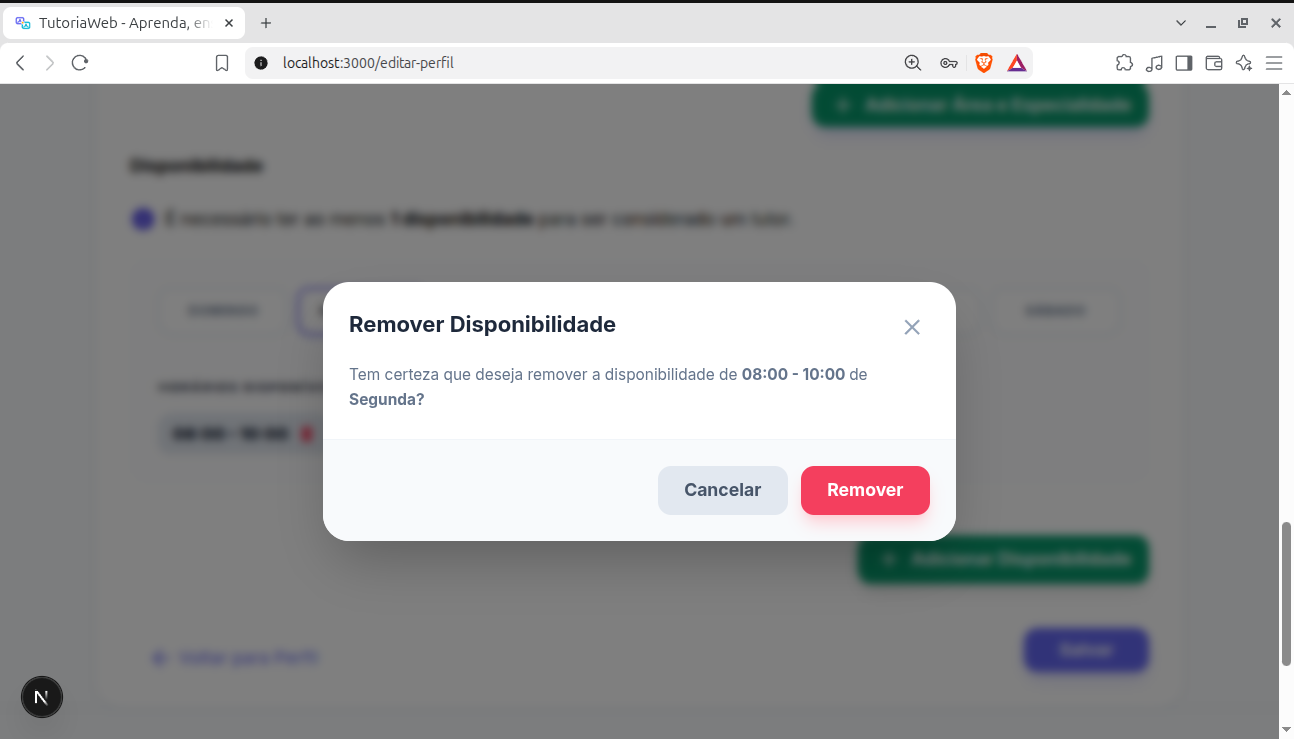
\includegraphics[width=1.9\textwidth, height=0.90\textheight, keepaspectratio]{figuras/modalApagarDisponibilidade.png}
    
    
        Fonte: Autoria própria.
        
        \vspace{0.2cm}
            
        \label{fig:modalApagarDisponibilidade}
    \end{figure}
\end{landscape}
\clearpage

Durante o desenvolvimento dessa US, os autores implementaram uma melhoria importante: não permitir que um tutor apague uma disponibilidade que possua solicitações pendentes ou sessões confirmadas. Nessa situação, o tutor deve cancelar a solicitação ou esperar um horário após a sessão para então prosseguir com a deleção. Uma mensagem de aviso é exibida ao usuário informando-o isso quando um dia em que alguma disponibilidade possua pendência é clicada. A mensagem pode ser observada na Figura \ref{fig:avisoDelecao}.

Nessa situação o tutor também não consegue apagar todas as áreas e especialidades que possui registradas, pois a aplicação não permite dados parciais como tutor, como ter somente disponibilidade ou ter somente área e especialidade. Portanto, ele continua como tutor até lidar com a solicitação ou até a sessão de tutoria ser feita.

Durante o desenvolvimento desta funcionalidade, foi notado pelo autores a necessidade de fazer uma melhoria na modelagem do banco de dados para melhor atender o gerenciamento de disponibilidades. Inicialmente o banco de dados possuia duas tabelas, ``SESSAO'' e ``SOLICITACAO'', onde foi planejado que o tutor criaria sessões e disponibilizaria os horários na sessão, enquanto o aprendiz iria solicitar participação nela. Entretanto, foi decidido que seria mais eficiente criar a tabela ``AGENDA'' para conter os registros de disponibilidade do tutor, e somente ao aceitar a solicitação do aluno cria-se a sessão.

Não houveram muitas dificuldades técnicas no \textit{frontend} dessas funcionalidades. O maior empecilho foi a criação do elemento visual de disponibilidade, que é um elemento com maior grau de complexidade em questão de lógica, visto que precisa mostrar os sete dias da semana e as disponibilidades de cada dia separadamente.

\begin{landscape}
    \setlength{\oddsidemargin}{\evensidemargin}
    \numeracaoPaisagem
    \begin{figure}[H]
        \centering
        \caption{Mensagem de aviso sobre deleção de disponibilidade.} 
        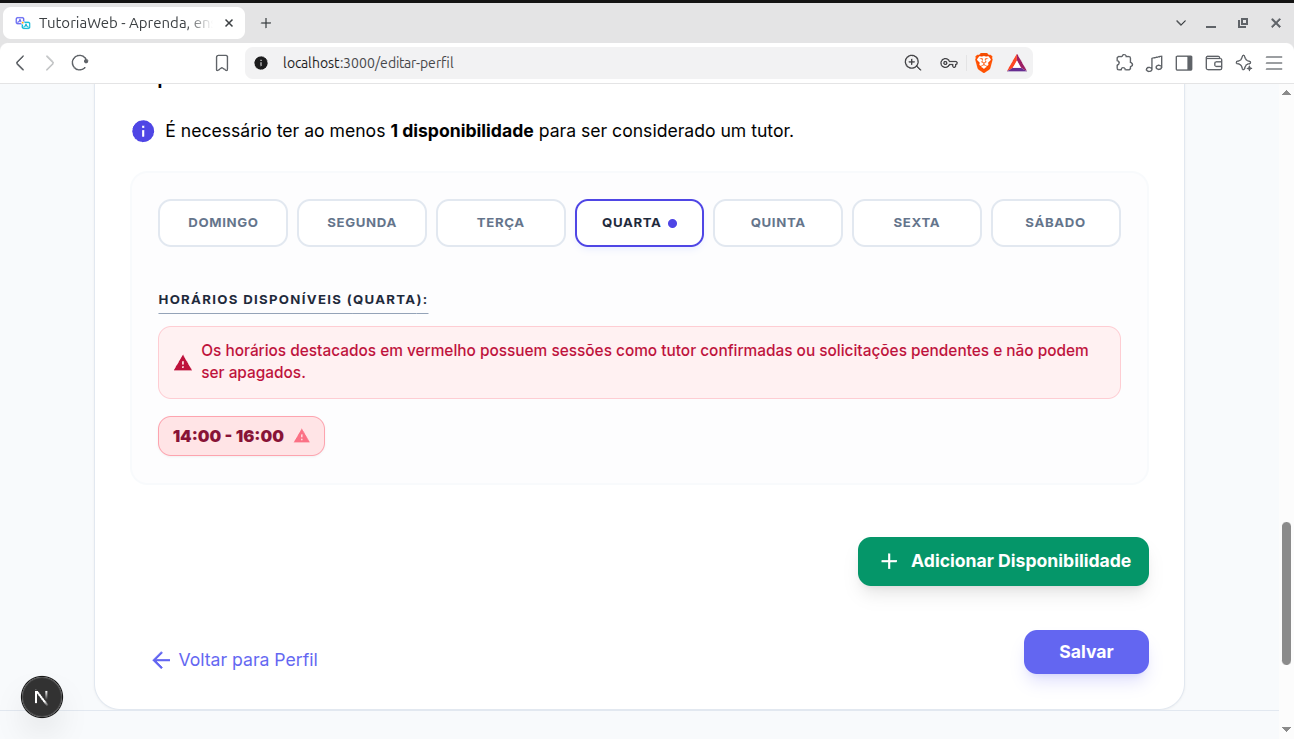
\includegraphics[width=1.9\textwidth, height=0.90\textheight, keepaspectratio]{figuras/avisoDelecao.png}
    
    
        Fonte: Autoria própria.
        
        \vspace{0.2cm}
            
        \label{fig:avisoDelecao}
    \end{figure}
\end{landscape}
\clearpage


\subsection[Funcionalidade 3: Agendamento de Tutorias]{Funcionalidade 3: Agendamento de Tutorias}

\subsubsection[US07: Solicitar Horário]{US07: Solicitar Horário}
\label{sec:us07}

A estimativa para o desenvolvimento dessa US era na Semana 4, de 29 de Março a 04 de Abril. O \textit{backend} foi desenvolvido principalmente no período do dia 2 de maio até o dia 8 de maio, havendo refatorações para melhorias de regras de negócios entre os dias 26 de maio e 11 de junho. O \textit{frontend} foi desenvolvido em partes.  No dia 8 de abril foi desenvolvida a \textit{modal} de solicitação de sessão, com dados simulados. Após isso, foi feito o desenvolvimento da página de edição de perfil e das páginas de busca e recomendação de tutores. Em 8 de maio foi feita a página de acompanhamento de solicitações. Novamente, o desenvolvimento foi pausado para priorização de outras US. O desenvolvimento foi retornado em 3 de junho e prosseguiu até 10 de junho. Em 18 de junho essa funcionalidade foi modificada a fins de se realizar melhorias, sendo completada em 29 de junho.

A solicitação de sessão de tutoria é feita na página do tutor, a qual é acessada clicado em seu \textit{card} na página de busca ou recomendação de tutores. Uma vez nessa página, o botão ``Solicitar Sessão'' pode ser clicado na sessão de disponibilidades, abrindo uma \textit{modal} em que são exibidos o mês atual e os dois meses seguintes. 

Dias em que o tutor possui disponibilidade podem ser clicados. Quando isso ocorre, o usuário pode selecionar uma área de conhecimento e uma especialidade dentre as que o tutor possui registradas, assim como um horário disponível naquele dia. Pode-se também marcar se a solicitação é recorrente. Uma solicitação recorrente, ao ser aceita pelo tutor, cria uma nova solicitação para o mesmo dia da semana e horário na semana seguinte. A \textit{modal} pode ser observada nas Figuras \ref{fig:modalSolicitacao} e \ref{fig:modalSolicitacao2}.

\begin{landscape}
    \setlength{\oddsidemargin}{\evensidemargin}
    \numeracaoPaisagem
    \begin{figure}[H]
        \centering
        \caption{\textit{Modal} de solicitação de sessão.} 
        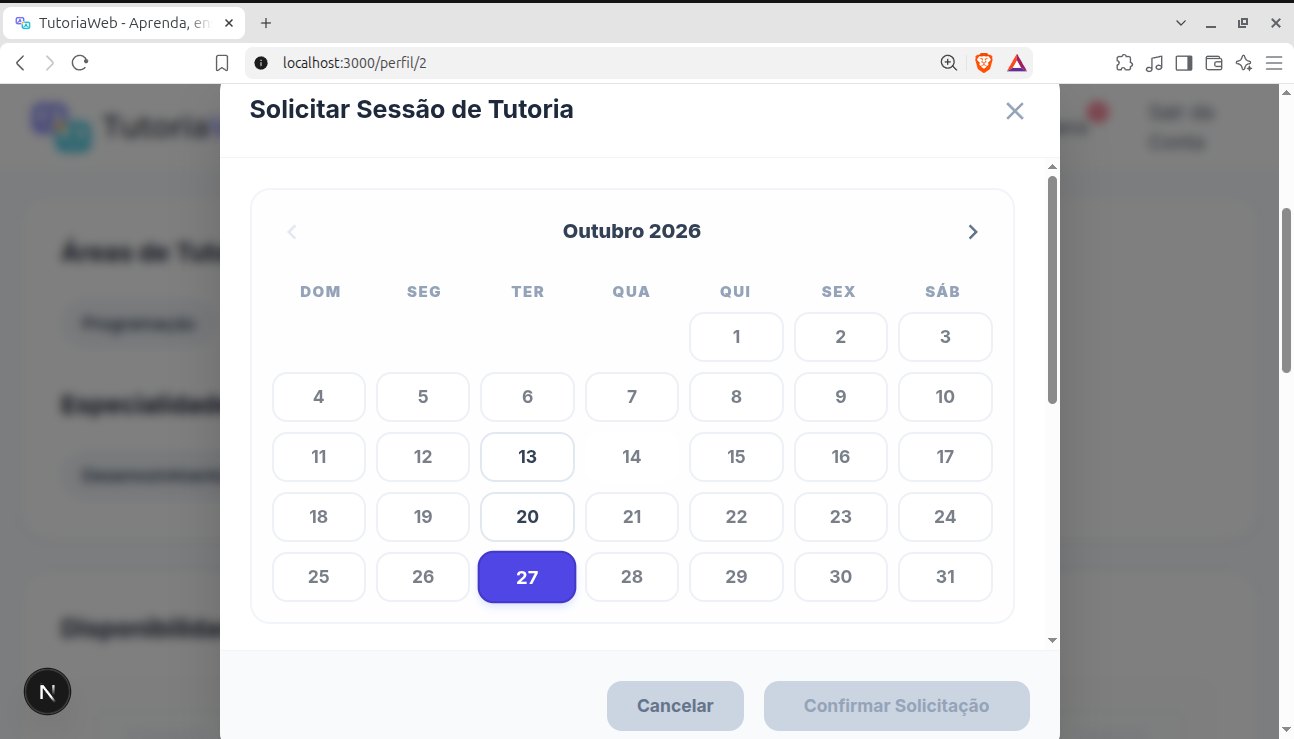
\includegraphics[width=1.9\textwidth, height=0.90\textheight, keepaspectratio]{figuras/modalSolicitacao.png}
    
    
        Fonte: Autoria própria.
        
        \vspace{0.2cm}
            
        \label{fig:modalSolicitacao}
    \end{figure}
\end{landscape}
\clearpage


\begin{landscape}
    \setlength{\oddsidemargin}{\evensidemargin}
    \numeracaoPaisagem
    \begin{figure}[H]
        \centering
        \caption{Continuação da \textit{modal} de solicitação de sessão.} 
        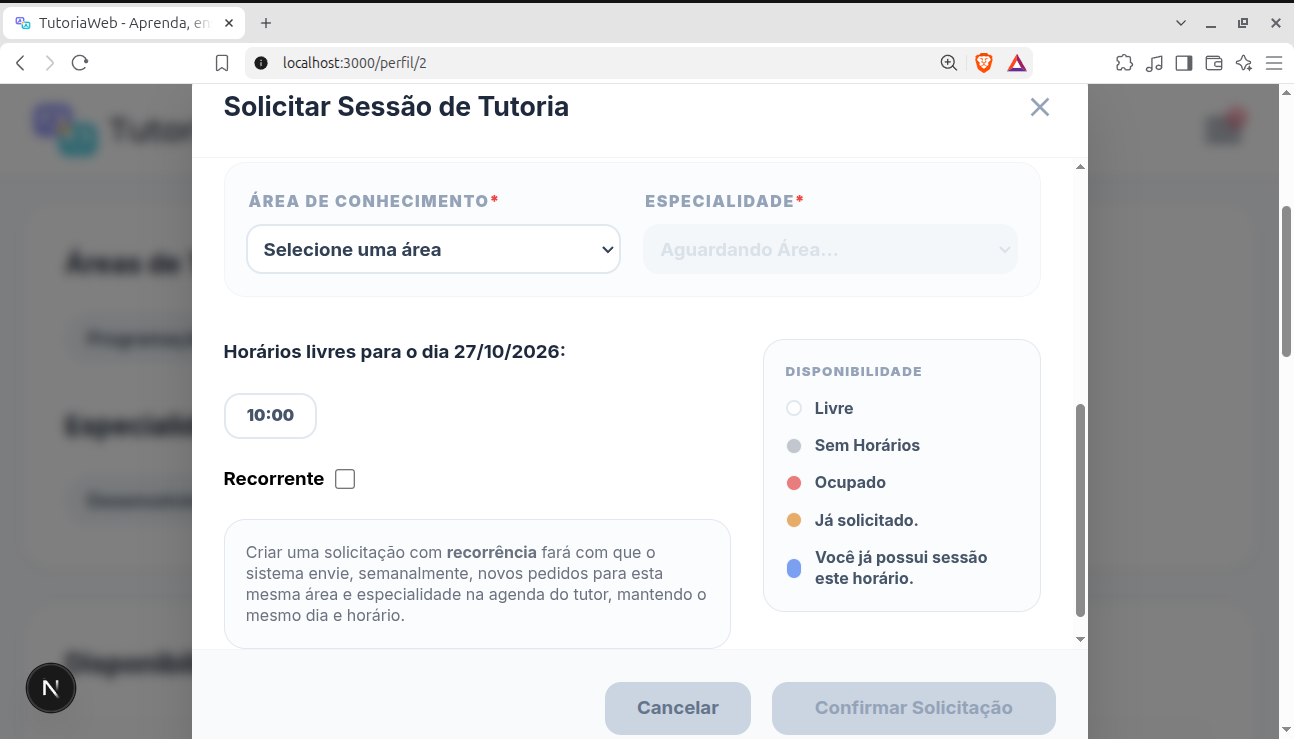
\includegraphics[width=1.9\textwidth, height=0.90\textheight, keepaspectratio]{figuras/modalSolicitacao2.png}
    
    
        Fonte: Autoria própria.
        
        \vspace{0.2cm}
            
        \label{fig:modalSolicitacao2}
    \end{figure}
\end{landscape}
\clearpage

O usuário pode então verificar o estado de sua solicitação na página de solicitações e sessões, acessível clicando no item ``Solicitações'' no menu do cabeçalho. Nessa página, ao clicar na aba ``Minhas Solicitações'', o usuário pode ver \textit{cards} com as informações da solicitação realizada. Solicitações em estado de pendência são exibidas nessa seção, enquanto que solicitações aceitas pelo tutor são exibidas na aba ``Sessões Aceitas como Aprendiz'', onde são exibidas as mesmas informações que o \textit{card} de ``Minhas Solicitações'', apenas mudando o valor do campo \textit{Status} para ``ACEITO''. Ambas as páginas podem ser observadas nas Figuras \ref{fig:paginaSolicitacao1}, \ref{fig:paginaSolicitacao2} e \ref{fig:paginaSolicitacao3}.

São feitas verificações de solicitações pendentes e das sessões confirmadas, tanto do usuário como tutor e aprendiz, quanto do tutor também nos papéis de tutor e aprendiz na \textit{modal} de solicitação de sessão.

O objetivo dessas verificações é impedir que um usuário solicite uma sessão em um dia e horário que já solicitou anteriormente com esse tutor e cuja solicitação ainda está pendente. Além disso, também impedir que um usuário solicite uma sessão em um dia e horário em que ele ou o tutor já possuem uma sessão. Caso um dia esteja totalmente ocupado na agenda de um tutor, ele é exibido em vermelho. Caso um horário possua uma solicitação pendente por parte do usuário, ele é colorido em amarelo. Por fim, caso um horário possua uma sessão confirmada, seja do lado do usuário ou do tutor, ele é exibido em vermelho. Em todos os casos, o usuário não consegue realizar a solicitação.

\begin{landscape}
    \setlength{\oddsidemargin}{\evensidemargin}
    \numeracaoPaisagem
    \begin{figure}[H]
        \centering
        \caption{Página de Gerenciamento de Sessões e Solicitações.} 
        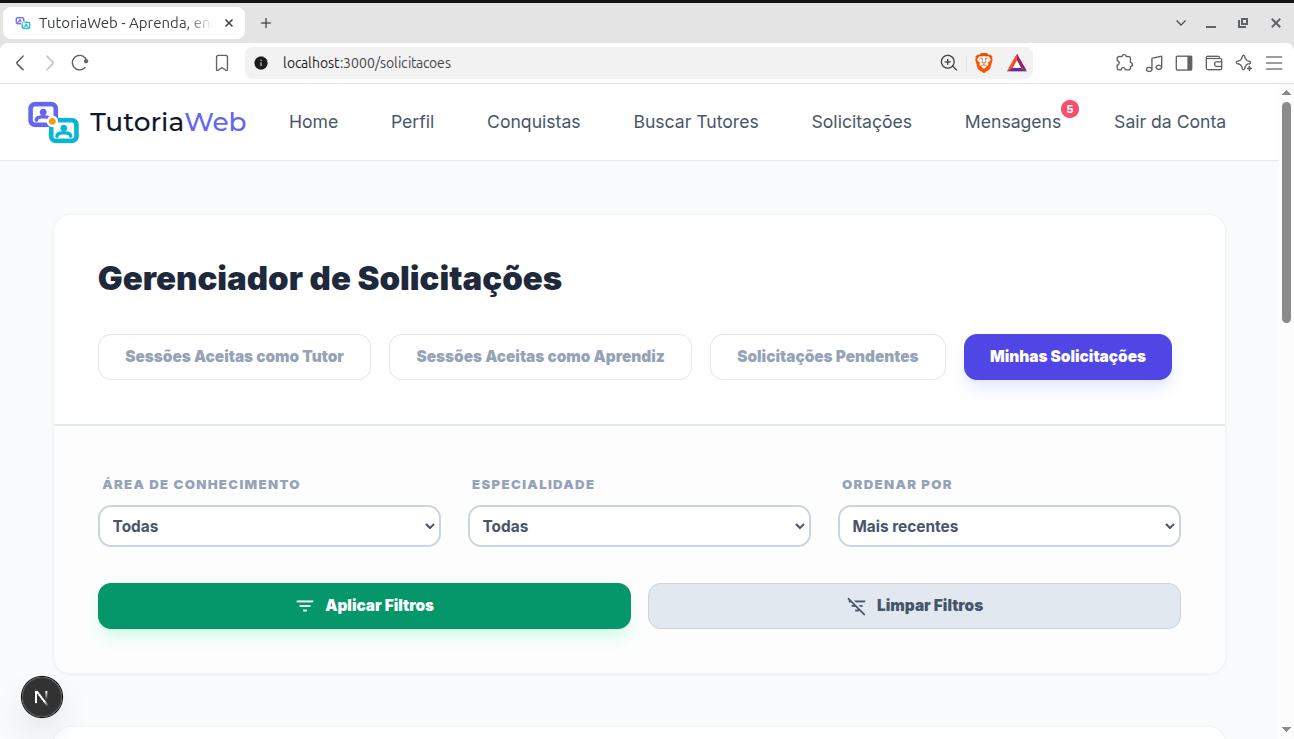
\includegraphics[width=1.9\textwidth, height=0.90\textheight, keepaspectratio]{figuras/paginaSolicitacao1.png}
    
    
        Fonte: Autoria própria.
        
        \vspace{0.2cm}
            
        \label{fig:paginaSolicitacao1}
    \end{figure}
\end{landscape}
\clearpage


\begin{landscape}
    \setlength{\oddsidemargin}{\evensidemargin}
    \numeracaoPaisagem
    \begin{figure}[H]
        \centering
        \caption{\textit{Cards} de solicitações de ``Minhas Solicitações''.} 
        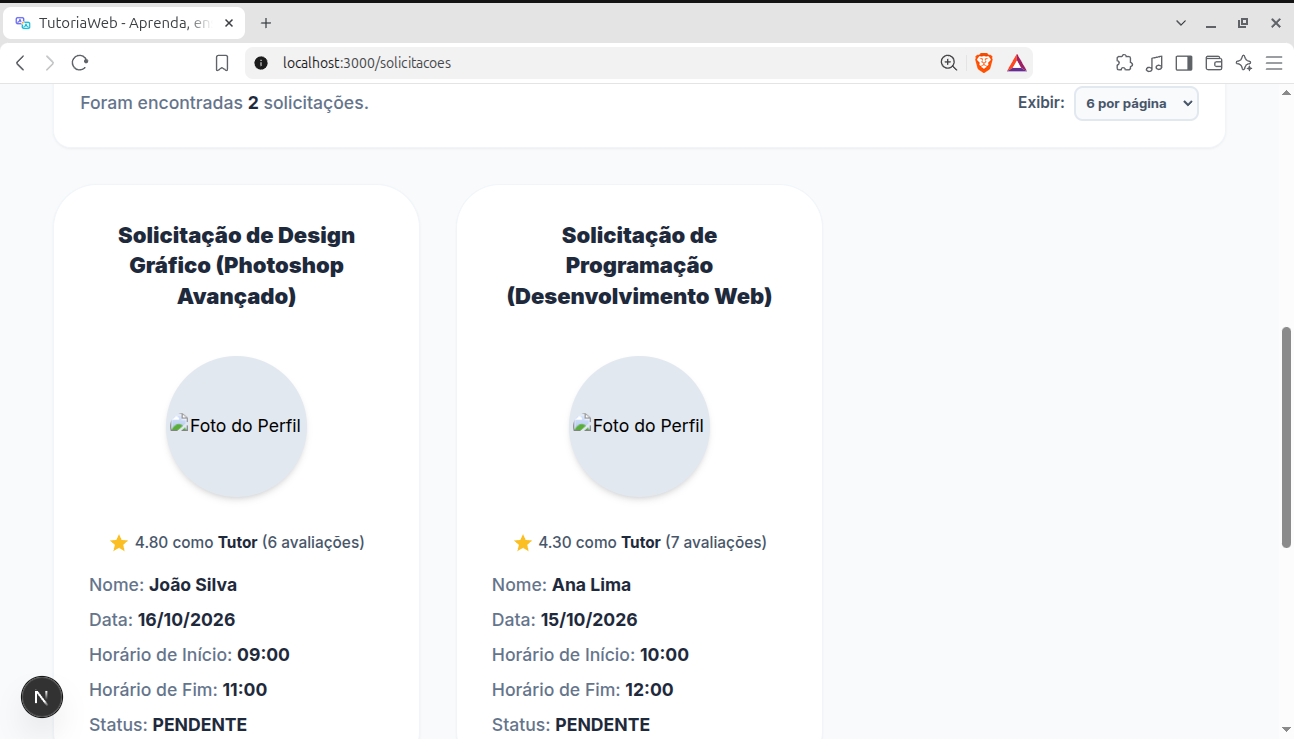
\includegraphics[width=1.9\textwidth, height=0.90\textheight, keepaspectratio]{figuras/paginaSolicitacao2.png}
    
    
        Fonte: Autoria própria.
        
        \vspace{0.2cm}
            
        \label{fig:paginaSolicitacao2}
    \end{figure}
\end{landscape}
\clearpage

\begin{landscape}
    \setlength{\oddsidemargin}{\evensidemargin}
    \numeracaoPaisagem
    \begin{figure}[H]
        \centering
        \caption{\textit{Cards} de solicitações de ``Sessões Aceitas como Aprendiz''.} 
        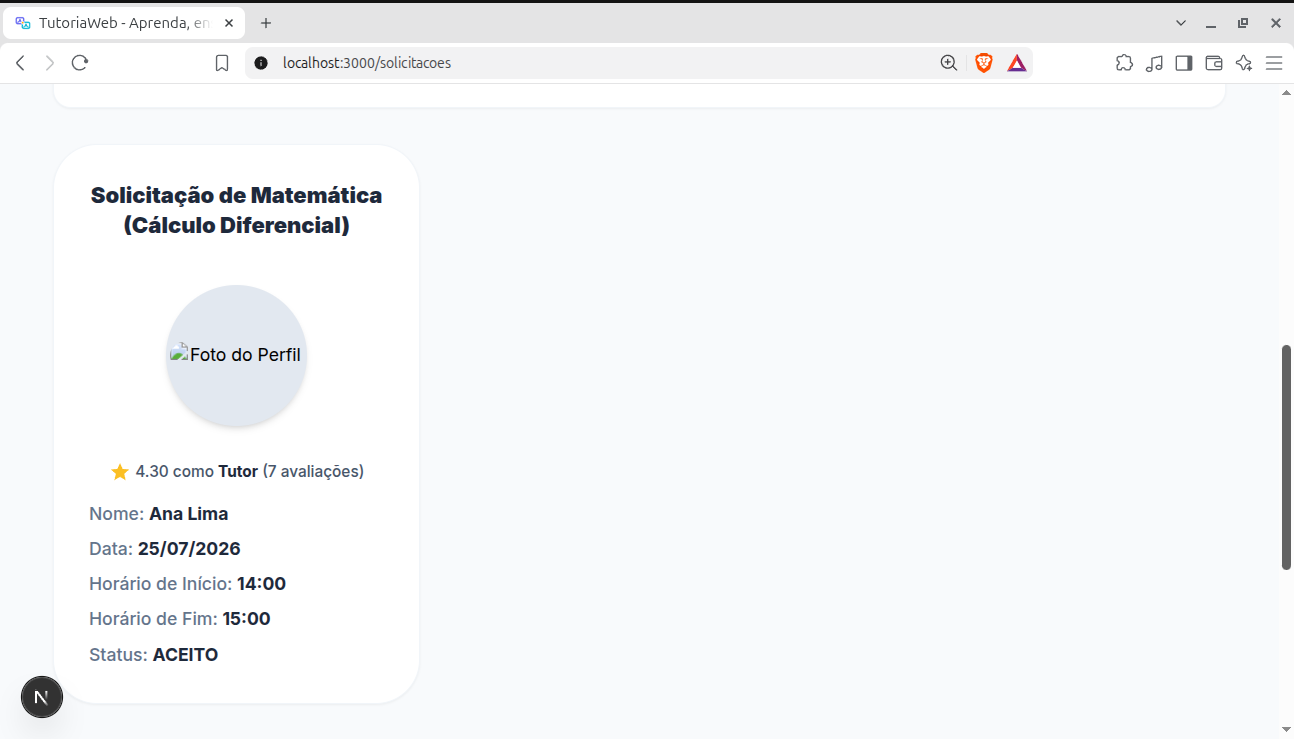
\includegraphics[width=1.9\textwidth, height=0.90\textheight, keepaspectratio]{figuras/paginaSolicitacao3.png}
    
        Fonte: Autoria própria.
        
        \vspace{0.2cm}
            
        \label{fig:paginaSolicitacao3}
    \end{figure}
\end{landscape}
\clearpage

Para atender ao CA04 dessa US (o tutor ser notificado de que recebeu uma nova solicitação de agendamento), foi utilizada a já mencionada notificação \textit{Snackbar}. Se o tutor está navegando na aplicação e um usuário realiza uma solicitação de sessão, uma \textit{Snackbar} aparece em sua tela informando-o que uma nova solicitação foi feita para ele.

Além disso, uma notificação visual é realizada no menu de cabeçalho, exibindo-se um ícone vermelho com a quantidade de solicitações pendentes do tutor. Ambas as notificações podem ser observadas na Figura \ref{fig:notificacoesSolicitacao}. 

A quantidade de solicitações pendentes do tutor é obtida através de uma requisição ao \textit{backend} que ocorre em um intervalo de 2 segundos e que retorna, além da quantidade de solicitações pendentes, a quantidade de sessões confirmadas que o usuário possui, como tutor e como aprendiz, e a quantidade de mensagens novas que possui. A fins de otimização, essa requisição só ocorre caso o usuário esteja com a aba da aplicação aberta no navegador.

Os autores optaram por realizar notificações visuais ao invés de e-mails por pensarem que os e-mails poderiam facilmente se tornar um \textit{spam}. Um tutor regularmente ativo na aplicação poderia receber vários e-mails de pedidos de solicitação, o que prejudicaria sua experiência.

Uma melhoria pensada e realizada durante o desenvolvimento foi a adição de solicitações recorrentes. Os autores julgaram ser uma boa adição à funcionalidade para atender a situação de um usuário que deseja marcar solicitações com o mesmo tutor, nos mesmos dias e horários, evitando que o mesmo realizasse todo o percurso de buscar o tutor e agendar as solicitações para realizar essa ação.

Durante o desenvolvimento dessa funcionalidade foram feitas alterações no banco de dados. Foram acrescentandos os atributos ``agendaId'', ``areaId'', ``especialidadeId'', ``recorrente'', ``dataPretendida'' e ``estado'' (que é um ENUM que aceita os valores ``ACEITO'', ``PENDENTE'', ``RECUSADO'' e ``RECORRENTE''). Isso foi feito para exibição de informações no \textit{card} de solicitação (área de conhecimento, especialidade, data pretendida e horário da solicitação), para possibilidade da funcionalidade de recorrência e para gerenciamento de estado da solicitação.

O desenvolvimento do \textit{backend} enfrentou obstáculos principalmente para estabelecer a nova modelagem do banco de dados, como descrito na Subseção \ref{sec:us05}.

O desenvolvimento do \textit{frontend} dessa US passou por dificuldades. Embora a tela de gerenciamento de solicitações e sessões tenha sido simples, a \textit{modal} de solicitações foi consideravelmente difícil de se fazer, desde o desafio de se exibir os meses e seus dias até a complexidade da verificação de solicitações e sessões na solicitação de uma sessão, sendo o componente visual mais complexo em termos de lógica de toda a aplicação. 

\begin{landscape}
    \setlength{\oddsidemargin}{\evensidemargin}
    \numeracaoPaisagem
    \begin{figure}[H]
        \centering
        \caption{Notificações de solicitação exibidas para o tutor.} 
        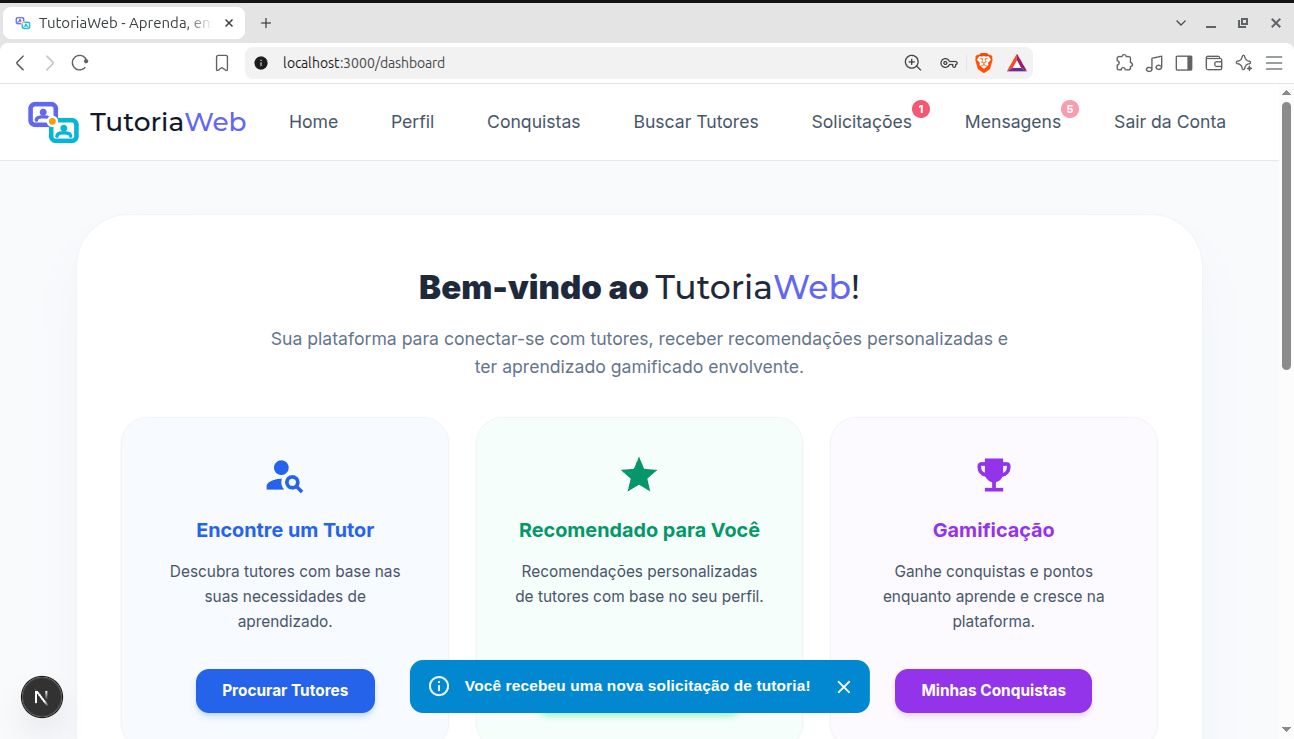
\includegraphics[width=1.9\textwidth, height=0.90\textheight, keepaspectratio]{figuras/notificacoesSolicitacao.png}
    
        Fonte: Autoria própria.
        
        \vspace{0.2cm}
            
        \label{fig:notificacoesSolicitacao}
    \end{figure}
\end{landscape}
\clearpage

\subsubsection[US08: Aceitar e Recusar Solicitação]{US08: Aceitar e Recusar Solicitação}

A estimativa inicial para o desenvolvimento dessas US era na Semana 5, de 05 a 11 de Abril. O \textit{backend} teve o desenvolvimento em paralelo com a Seção \ref{sec:us07}, entre os dias 02 e 08 de maio, e refatorações de regras de negócios futuras entre os dias 26 de maio e 11 de junho. O \textit{frontend} começou a ser desenvolvido em 11 de junho e terminou em 16 de junho.

Quando uma solicitação é feita para um tutor, ela aparece na aba ``Solicitações Pendentes'' da página de solicitações. Nessa aba são exibidas as informações da solicitação, botões para  e também o prazo que o tutor tem para responder à ela, em horas, conforme pode ser observado na Figura \ref{fig:cardSolicitacaoPendente}.

Ao clicar em algum dos botões, uma \textit{modal} é exibida na tela para confirmar a ação. Independente da ação do tutor, o resultado é informado ao aprendiz através de uma notificação \textit{Snackbar} em sua tela.

Caso o tutor recuse a solicitação, e não exista sessão confirmada para o dia e horário solicitado, o aprendiz pode ir até a página do perfil do tutor e realizar a solicitação novamente.

Caso o tutor aceite a solicitação, é registrada uma sessão no banco de dados, que pode ser visualizada na aba ``Sessões Aceitas como Tutor'' para o tutor e na aba ``Sessões Aceitas como Aprendiz'' para o aprendiz. É também exibida uma notificação visual no item ``Solicitações'' no menu do cabeçalho na forma de um ícone verde com a quantidade de sessões confirmadas para ambos, seja como tutor ou como aprendiz, que ainda irão acontecer. O \textit{card} de sessão pode ser observado na Figura \ref{fig:cardSessaoAceita}, enquanto que a notificação visual pode ser observada na Figura \ref{fig:notificacaoSessaoConfirmada}.

Essa forma de notificação, ao invés de notificação por e-mail, ocorreu pelo mesmo motivo já explicado já explicado anteriormente: um aprendiz ou um tutor regularmente ativo na aplicação poderia receber vários e-mails de recusa ou confirmação de sessão, facilmente se tornando um \textit{spam} e prejudicando a experiência do usuário.

Foram realizadas alterações no banco de dados durante o desenvolvimento. A tabela ``SESSAO'' recebeu os atributos ``areaId'', ``especialidadeId'' e ``dataSessao'' para exibição das informações da área de conhecimento, especialidade e a data da sessão no \textit{card} dela.

Não houve dificuldades no desenvolvimento no \textit{backend} e \textit{frontend} dessa US.

\begin{landscape}
    \setlength{\oddsidemargin}{\evensidemargin}
    \numeracaoPaisagem
    \begin{figure}[H]
        \centering
        \caption{\textit{Card} de solicitações pendente.} 
        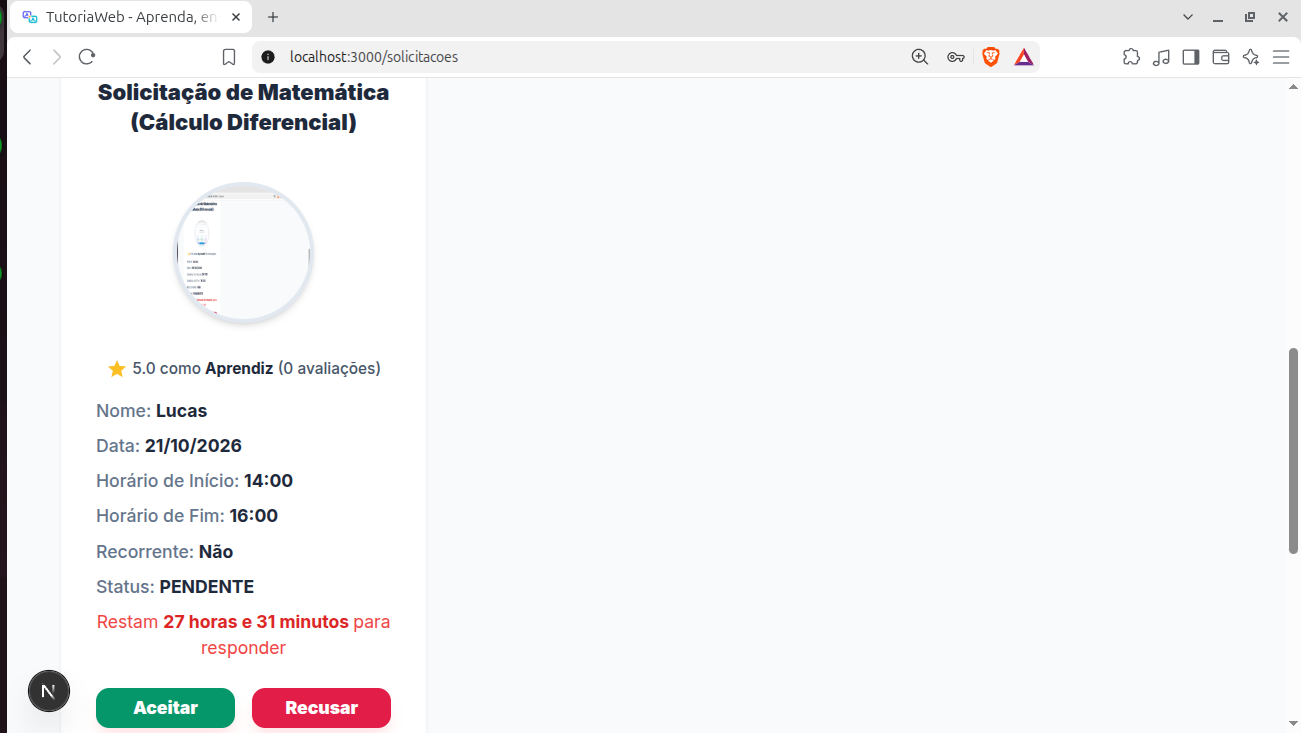
\includegraphics[width=1.9\textwidth, height=0.90\textheight, keepaspectratio]{figuras/cardSolicitacaoPendente.png}
    
        Fonte: Autoria própria.
        
        \vspace{0.2cm}
            
        \label{fig:cardSolicitacaoPendente}
    \end{figure}
\end{landscape}
\clearpage

\begin{landscape}
    \setlength{\oddsidemargin}{\evensidemargin}
    \numeracaoPaisagem
    \begin{figure}[H]
        \centering
        \caption{\textit{Card} de sessão aceita.} 
        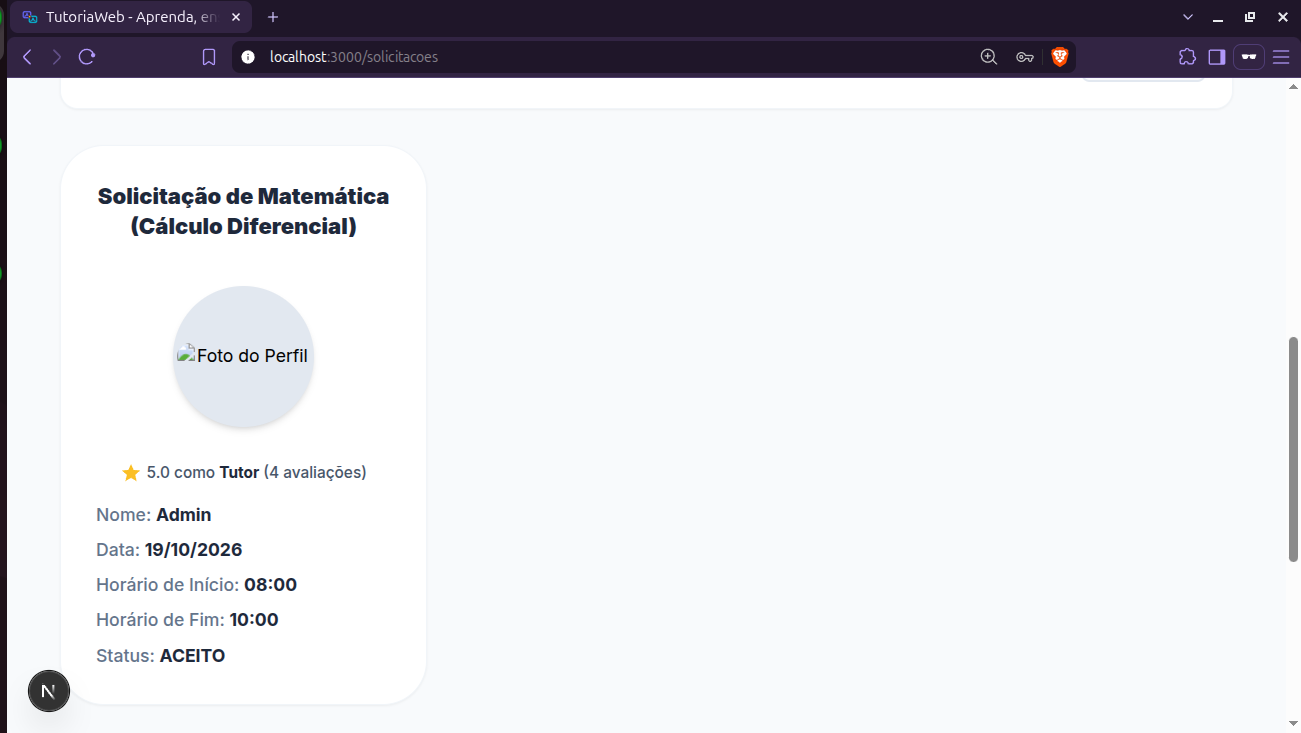
\includegraphics[width=1.9\textwidth, height=0.90\textheight, keepaspectratio]{figuras/cardSessaoAceita.png}
    
        Fonte: Autoria própria.
        
        \vspace{0.2cm}
            
        \label{fig:cardSessaoAceita}
    \end{figure}
\end{landscape}
\clearpage

\begin{landscape}
    \setlength{\oddsidemargin}{\evensidemargin}
    \numeracaoPaisagem
    \begin{figure}[H]
        \centering
        \caption{Notificação de sessão aceita no menu do cabeçalho.} 
        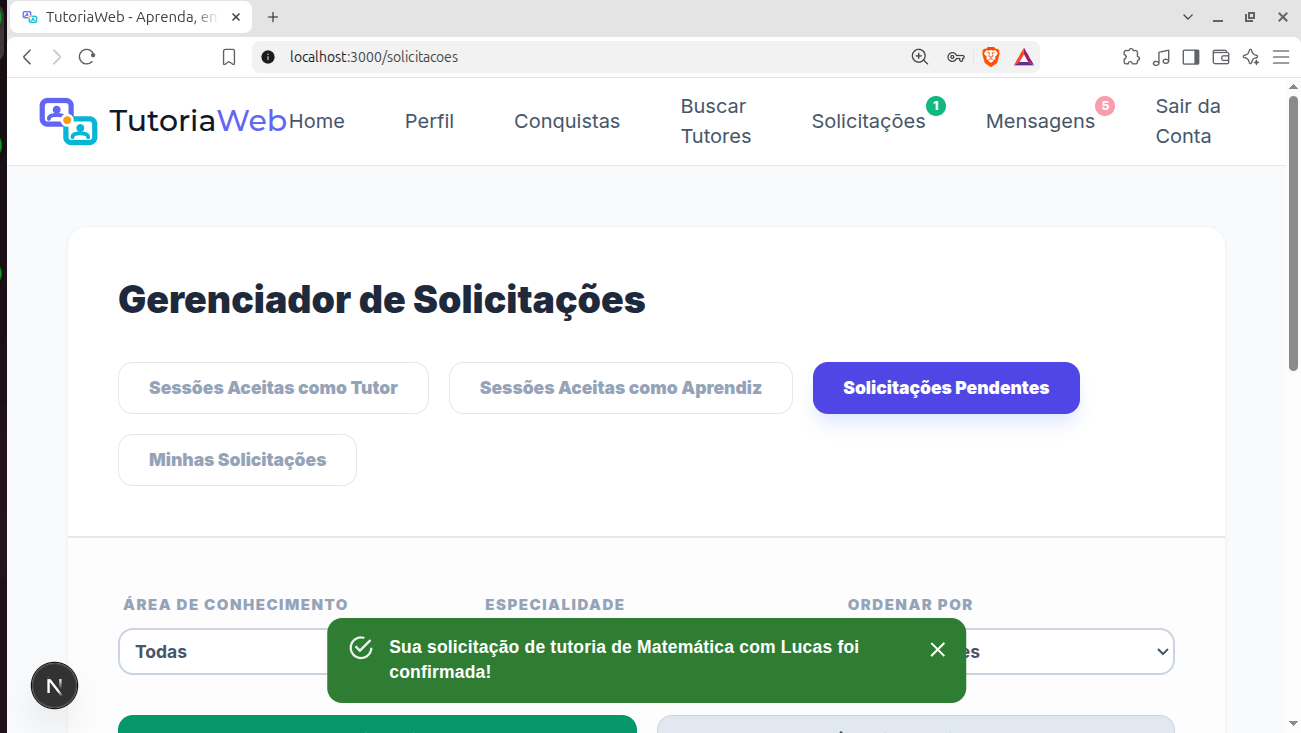
\includegraphics[width=1.9\textwidth, height=0.90\textheight, keepaspectratio]{figuras/notificacaoSessaoConfirmada.png}
    
        Fonte: Autoria própria.
        
        \vspace{0.2cm}
            
        \label{fig:notificacaoSessaoConfirmada}
    \end{figure}
\end{landscape}
\clearpage

\subsubsection[US09: Expirar Solicitação]{US09: Expirar Solicitação}

A estimativa inicial para o desenvolvimento dessas US era na Semana 5, de 05 a 11 de abril, juntamente com a US08. O \textit{backend} começou a ser desenvolvido em 2 de maio, sendo posteriormente refotorado em 10 e 11 de junho para mudanças na regra de negócio, 24 de agosto para correção no fuso horário do tempo de validade e 26 de agosto para implementar envio de e-mails e deleção de solicitações expiradas do banco de dados. Não houve desenvolvimento de \textit{frontend} para essa funcionalidade.

Quando uma solicitação é criada no banco de dados, é feito o cálculo de seu prazo de expiração. Inicialmente, seguiu-se o CA02 da US, com  o prazo de validade de uma solicitação sendo de 24 horas após sua criação.

Entretanto, os autores pensaram em melhorias que alteraram a regra de negócio. Caso uma solicitação fosse para o dia seguinte, poderia ocorrer de o prazo de validade ultrapassar o horário de início da sessão, tornando-o sem sentido. Além disso, considerou-se também a situação de uma solicitação ser feita na sexta-feira. Nesse caso, com a regra de negócio original, a validade iria até um determinado horário no sábado. Entretanto, os autores consideraram que um tutor poderia não acessar a aplicação nos fins de semana. Dessa maneira, a solicitação iria expirar sem o tutor sequer ter ciência de sua existência.

Isso levou à refatorações na funcionalidade, de modo que as regras de negócio para o cálculo da validade passaram a ser essas:

\begin{itemize}

\item Caso a solicitação seja para o dia seguinte, ela permanece válida até o horário de início da sessão pretendida;

\item Caso a solicitação seja para uma data posterior, ela permanece válida até as 23:59 do dia seguinte à sua criação;

\item Caso a solicitação seja para a semana seguinte e os dias seguintes sejam sábado e domingo, ela permanece válida até as 23:59 de segunda-feira, exceto se a solicitação for agendada para a própria segunda-feira, situação em que permanece válida até o horário de início da sessão pretendida.

\end{itemize}

Se uma solicitação expira, é enviado um e-mail tanto para o tutor quanto para o aprendiz os notificando dessa ocorrência, cujo texto é diferente para se adequar aos diferentes papéis. Como exemplo, o e-mail enviado para o aprendiz pode ser observado na Figura \ref{fig:emailExpiracaoSolicitacao}.

\begin{landscape}
    \setlength{\oddsidemargin}{\evensidemargin}
    \numeracaoPaisagem
    \begin{figure}[H]
        \centering
        \caption{E-mail informativo sobre a expiração de uma solicitação para o aprendiz.} 
        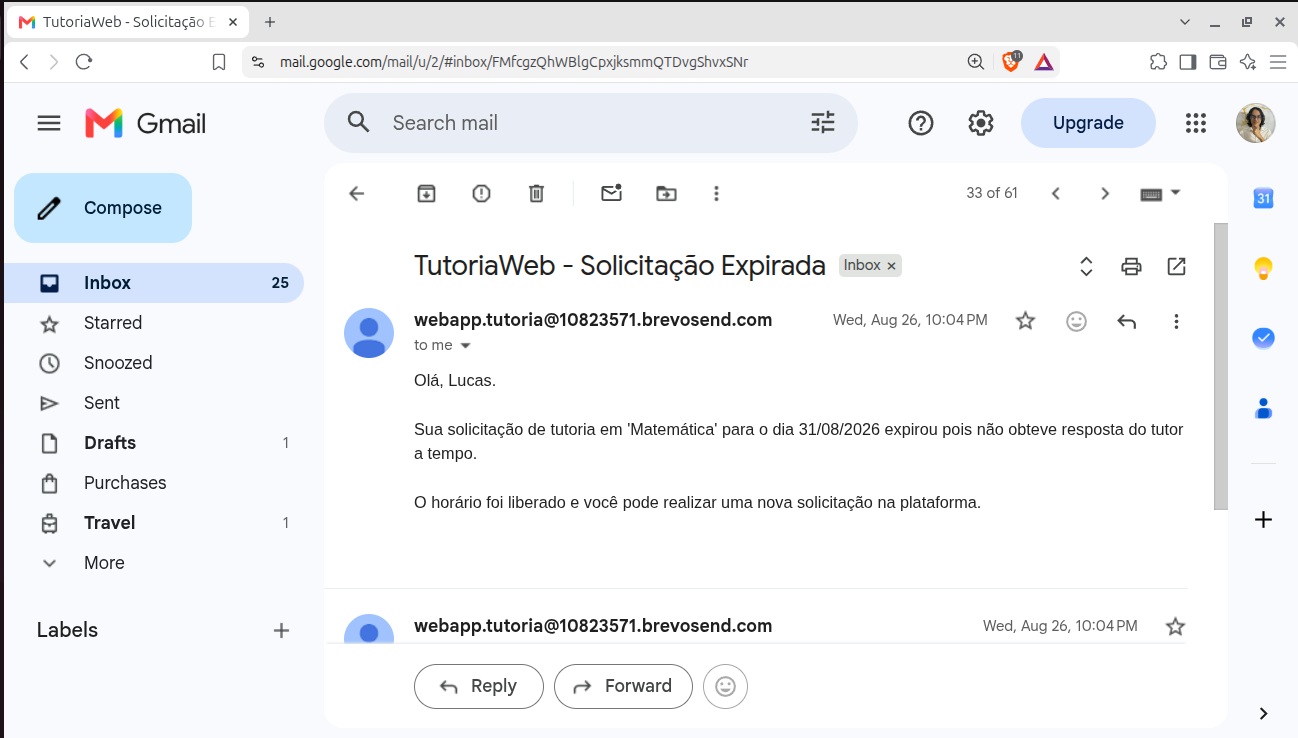
\includegraphics[width=1.9\textwidth, height=0.90\textheight, keepaspectratio]{figuras/emailExpiracaoSolicitacao.png}
    
        Fonte: Autoria própria.
        
        \vspace{0.2cm}
            
        \label{fig:emailExpiracaoSolicitacao}
    \end{figure}
\end{landscape}
\clearpage

Houve uma dificuldade no desenvolvimento dessa US. No \textit{frontend} o horário de expiração exibido no \textit{card} da solicitação estava incorreto. Após investigação no código, não foram encontradas falhas na lógica do cálculo. A falha na verdade estava no próprio Django. O fuso horário do Django, por padrão, não é o mesmo do Brasil, causando a diferença de horas. Quando isso foi ajustado, os horários foram corrigidos.

\subsection[Funcionalidade 4: Sistema de Avaliação]{Funcionalidade 4: Sistema de Avaliação}

\subsubsection[US10: Avaliar Tutor e US11: Avaliar Aprendiz]{US10: Avaliar Tutor e US11: Avaliar Aprendiz}

Essas US serão descritas na mesma subseção, visto que são funcionalmente idênticas. A estimativa inicial para o desenvolvimento da US10 era na Semana 7, de 19 a 25 de abril, enquanto que a US11 seria desenvolvida na Semana 8, de 26 a 02 de maio. O \textit{backend} foi desenvolvido no período de entre 18 e 20 de maio, havendo refatorações de 20 de julho à 10 de agosto. O desenvolvimento do \textit{frontend} começou em 01 de maio, com a criação da \textit{modal}, finalizada em 02 de maio. A integração com o \textit{backend} foi feita em 12 de agosto.

Assim que o usuário faz \textit{login} na aplicação, é feita uma requisição ao \textit{backend} para se obter quais sessões estão pendentes de avaliação por parte do mesmo. Caso existam, são exibidas \textit{modais}, uma por vez, com informações relevantes, como nome e foto do tutor ou do aprendiz, o assunto da sessão e a data e horário em que foi feita. O usuário pode, então, avaliar o outro parcicipante com uma nota de 1 a 5 estrelas, bem como escrever um comentário de até 200 caracteres. O texto muda de acordo com o papel do usuaŕio que está avaliando a sessão (tutor ou aprendiz). Como exemplo, a \textit{modal} de avalição de um tutor pode ser observada nas Figuras \ref{fig:modalAvaliacao1} e \ref{fig:modalAvaliacao2}.

Para forçar o usuário a realizar a avaliação, a \textit{modal} não apresenta botão ou ícone para ser fechada, e clicar fora dela também não a fecha. Assim que uma sessão é avaliada, a próxima é exibida para avaliação logo em seguida. O usuário somente consegue utilizar a aplicação após avaliar todas as sessões pendentes.

As avaliações podem ser visualizadas em uma seção dedicada à elas na página de perfil, localizada na parte inferior. Caso um usuário seja tutor na aplicação é possível visualizar tanto avaliações como aprendiz como quanto tutor, sendo possível filtrar e ordenar os resultados. Caso um usuário não tenha redigido um comentário, o texto ``O usuário não escreveu comentário para essa avaliação'' é exibido. A seção de avaliações pode ser observada na Figura \ref{fig:secaoAvaliacoes}. Vale notar que, seguindo o CA05, a avaliação só se torna visível para o outro participante (e no perfil público dele) após ele também ter feito a avaliação sobre o usuário nessa sessão ou após um prazo de 48 horas ter passado (o que ocorrer primeiro).

\begin{landscape}
    \setlength{\oddsidemargin}{\evensidemargin}
    \numeracaoPaisagem
    \begin{figure}[H]
        \centering
        \caption{\textit{Modal} de avaliação de tutor.} 
        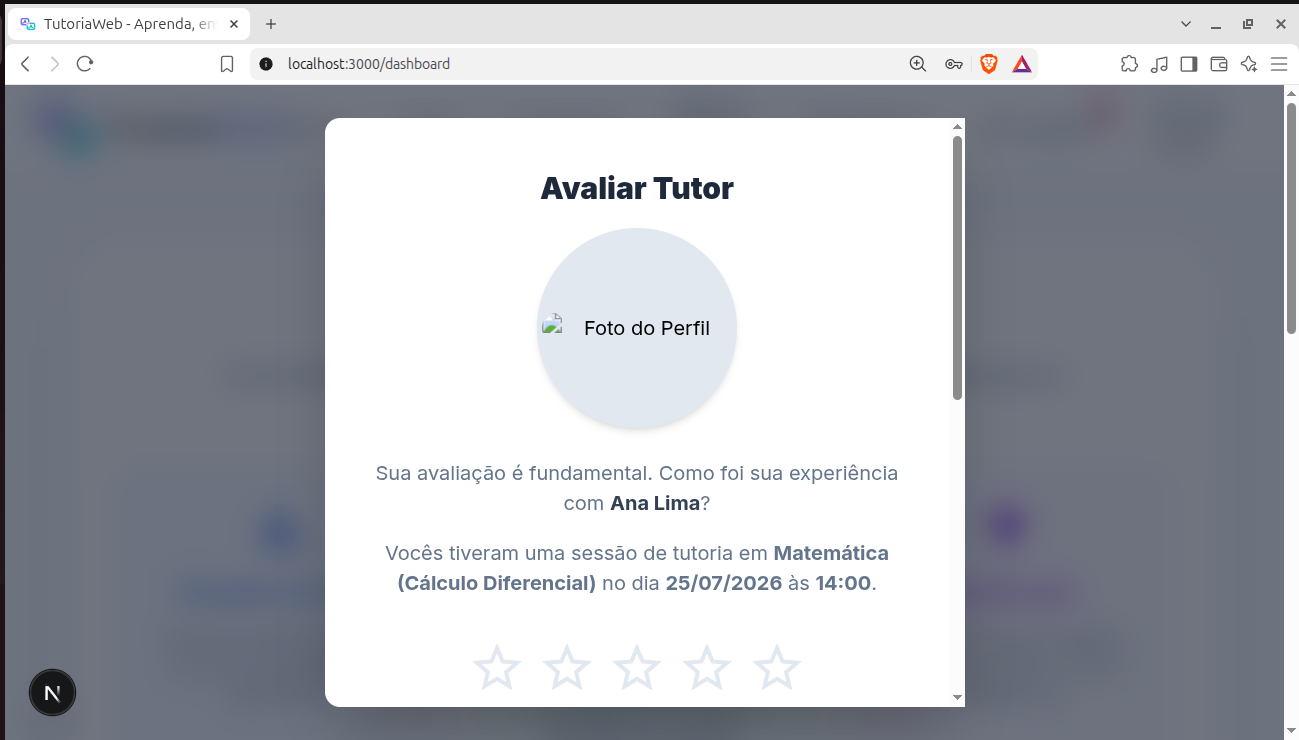
\includegraphics[width=1.9\textwidth, height=0.90\textheight, keepaspectratio]{figuras/modalAvaliacao1.png}
    
        Fonte: Autoria própria.
        
        \vspace{0.2cm}
            
        \label{fig:modalAvaliacao1}
    \end{figure}
\end{landscape}
\clearpage

\begin{landscape}
    \setlength{\oddsidemargin}{\evensidemargin}
    \numeracaoPaisagem
    \begin{figure}[H]
        \centering
        \caption{Continuação da \textit{modal} de avaliação de tutor.} 
        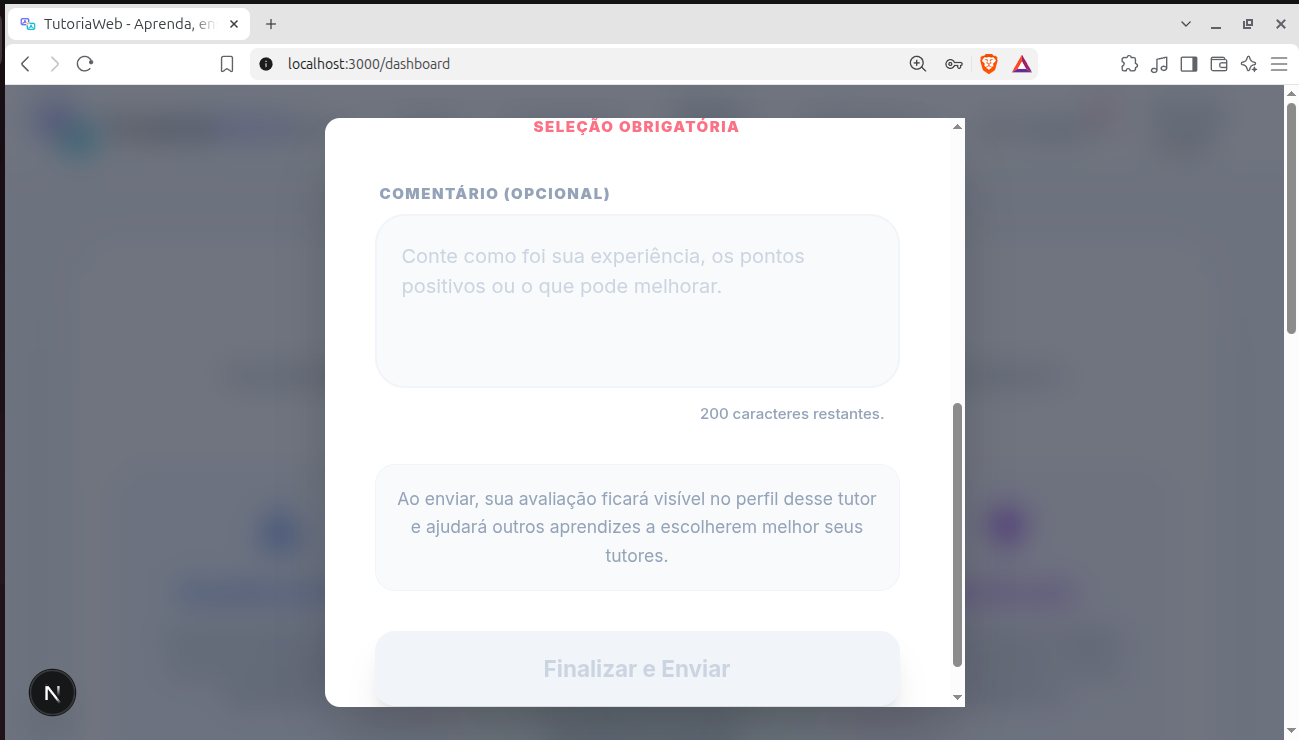
\includegraphics[width=1.9\textwidth, height=0.90\textheight, keepaspectratio]{figuras/modalAvaliacao2.png}
    
        Fonte: Autoria própria.
        
        \vspace{0.2cm}
            
        \label{fig:modalAvaliacao2}
    \end{figure}
\end{landscape}
\clearpage

\begin{landscape}
    \setlength{\oddsidemargin}{\evensidemargin}
    \numeracaoPaisagem
    \begin{figure}[H]
        \centering
        \caption{Seção de avaliações na página de perfil.} 
        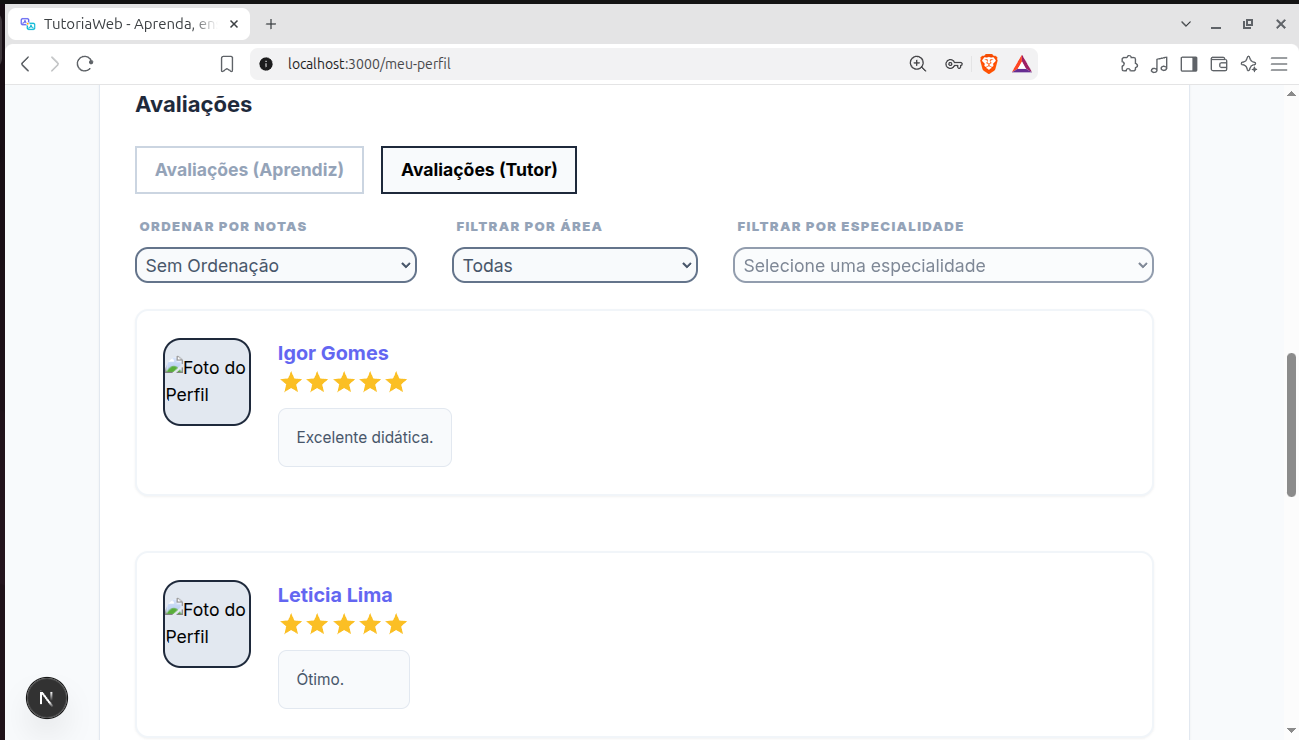
\includegraphics[width=1.9\textwidth, height=0.90\textheight, keepaspectratio]{figuras/secaoAvaliacoes.png}
    
        Fonte: Autoria própria.
        
        \vspace{0.2cm}
            
        \label{fig:secaoAvaliacoes}
    \end{figure}
\end{landscape}
\clearpage

Visando incentivar o engajamento por meio da gamificação, propôs-se um aprimoramento para esta US: a atribuição automática de 50 pontos ao perfil do usuário sempre que este realizar uma avaliação, independentemente se atua como tutor ou aprendiz na sessão avaliada.

Houve uma mudança no banco de dados durante o desenvolvimento dessa funcionalidades: o atributo ``comentario'' nas tabelas ``AVALIACAO\_TUTOR'' e ``AVALIACAO\_APRENDIZ'' teve seu limite de caracteres aumentado para 200. A justificativa para isso é que 100 caracteres poderiam não ser o suficiente para uma crítica mais aprofundada. Além disso, a fim de se implementar as verificações para tornar uma avaliação pública, foram acrescentados o atributos ``sessaoId'' e ``dataCriacao'', sendo o primeiro usado para verificar se existe a avaliação realizada pelo outro participante da sessão, e o segundo usado para verificar se as 48 horas já se passaram. Foi também acrescentado o atributo ``notaAvaliacao'' na tabela ``TUTOR'' para armazenamento da nota média como tutor de um usuário.

Não houve dificuldades para \textit{backend} e \textit{frontend} dessas funcionalidades.

\subsubsection[US12: Ver Reputação]{US12: Ver Reputação}

A estimativa inicial para o desenvolvimento dessa US era na Semana 8 de 26 a 02 de maio, juntamente com a US11. O \textit{frontend} foi desenvolvido em 1 de junho.

A reputação de um usuário como tutor e como aprendiz pode ser visualizada em diferentes partes da aplicação. Na página de perfil são exibidos a avaliação média como aprendiz e como tutor, acompanhada da quantidade de avaliações públicas realizadas por outros usuários nesses papéis, sendo a avaliação como tutor exibida somente se o usuário é considerado um tutor na aplicação, de acordo com os critérios já mencionados na Subseção \ref{sec:us04}. As reputações podem ser observadas na Figura \ref{fig:telaPerfil1}.

Inicialmente ambas as notas inicialmente começam com o valor máximo, 5.0, sendo alteradas conforme as avaliações dos usuários são feitas. A nota somente é alterada após a avaliação se tornar pública. Todas as avaliações são consideradas no cálculo da nota média de avaliação.

Os autores pensaram em uma melhoria para essa funcionalidade, que seria exibi-las também nos \textit{cards} de solicitação e de sessões confirmadas, de acordo com o contexto. Por exemplo, a reputação do usuário como aprendiz é exibida no \textit{card} de solicitação, a fim de ajudar o tutor em sua decisão de aceitar ou recusar. Por outro lado, a reputação de um usuário como tutor é exibida no \textit{card} de sessão confirmada na aba "Sessões Aceitas como Aprendiz". A reputação em uma solicitação pendente como aprendiz pode ser observada na Figura \ref{fig:paginaSolicitacao2}.

Não houve dificuldade no desenvolvimento do \textit{frontend} e do \textit{backend} dessa US.

\subsection[Funcionalidade 5: Comunicação]{Funcionalidade 5: Comunicação}

\subsubsection[US13: Enviar Mensagem]{US13: Enviar Mensagem}

A estimativa inicial para o desenvolvimento dessa US era na Semana 9, de 3 a 9 de maio. O \textit{backend} foi desenvolvido principalmente em 24 de maio de 25, porém houve refatorações nos dias 12, 13 e 17 de agosto e uma ultima modificação no dia 11 de setembro. O \textit{frontend} começou em 12 de agosto e foi completado em 17 de agosto.

A comunicação por mensagens é iniciada quando um usuário envia uma mensagem para um tutor. Isso é feito é feito navegando até a página do perfil do tutor e clicando no botão ``Enviar Mensagem''. Fazer isso causa a exibição de uma \textit{modal} na tela, permitindo a escrita da mensagem. A \textit{modal} pode ser observada na Figura \ref{fig:modalMensagens}.

Após a mensagem ser enviada, uma comunicação entre o tutor e o aprendiz é iniciada, podendo ser acessada na página de mensagens ao se clicar na opção ``Mensagens'' no menu do cabeçalho. Ambos são notificados do recebimento de novas mensagens através de um ícone vermelho na opção do menu de cabeçalho, que contém a quantidade total de mensagens não lidas pelo usuário. Essa notificação pode ser vista na Figura \ref{fig:paginaSolicitacao1}.

Na página de mensagens, o usuário pode ver todas as comunicações que possui com outros usuários. Ao clicar em uma delas, é exibido o histórico de mensagens é exibido, sendo as mais recentes exibidas primeiro. É feita uma distinção visual entre as mensagens, sendo as do usuário logado exibidas à direita e em roxo e as do outro participante exibidas à esquerda e em cinza. Ao se subir a janela de mensagens, as mensagens mais antigas são buscadas do banco de dados e exibidas. A janela de mensagens pode ser observada na Figura \ref{fig:janelaMensagens}.

A fim de se carregar as mensagens novas das comunicações que o usuário possui, é feita uma requisição ao \textit{backend} de 2 em 2 segundos, feita somente quando o usuário está na página de mensagens. Caso o usuário tenha mensagens não lidas de outros usuários, um ícone vermelho com a quantidade de mensagens novas é exibido no \textit{card} da respectiva comunicação. Caso sejam mensagens novas da comunicação selecionada, elas são exibidas na tela. Isso pode ser observado na Figura \ref{fig:janelaMensagens}. O ícone só desaparece caso o usuário clique na comunicação e visualize as mensagens. Nesse caso, uma requisição ao \textit{backend} é realizada para alterar o estado delas para lido.

Essa requisição se difere da requisição mencionada na Subseção \ref{sec:us07}, que retorna o total de mensagens não lidas, enquanto a requisição da página de mensagens retorna a quais comunicações cada mensagem pertence.

A arquitetura inicial do módulo de mensagens passou por reestruturações técnicas relevantes. A principal alteração consistiu na substituição do uso de \textit{Enums} para a identificação do remetente, adotando-se, em seu lugar, o relacionamento direto por meio do \textit{id} do usuário que originou a ação. Além disso, introduziu-se um atributo booleano na entidade de mensagem com o propósito de indicar de forma explícita se o conteúdo já foi visualizado pelo destinatário.

Houveram dificuldades no desenvolvimento dessa US, sendo a mais difícil de ser completada de toda a aplicação. Isso se deve ao fato de nenhum dos autores possuírem experiência prévia no desenvolvimento uma comunicação por mensagens.

No \textit{frontend} houveram dúvidas de como obter o histórico de mensagens da comunicação, visto que carregar todas as mensagens em uma única requisição poderia torná-la lenta, além de ineficiente, visto que o usuário poderia estar interessado em ler apenas as mensagens mais recentes. Após pesquisa, foi adotada a solução de paginar o \textit{endpoint GET} de mensagens de uma comunicação específica, de modo a trazer as mais recentes primeiro e, caso o usuário role o histórico para cima, novas requisições serem feitas, trazendo as mensagens mais antigas.

Outra dúvida foi como obter as mensagens enviadas pelos usuários enquanto ambos estão com a comunicação selecionada, a fim de, de fato, se obter uma interação. A solução foi usar a citada requisição para se obter as mensagens em um intervalo de 2 segundos. Esse intervalo foi considerado ideal pois permite um carregamento rápido de mensagens ao mesmo tempo que não é curto o suficiente para sobrecarregar o servidor do \textit{backend}.

Outra dificuldade foi na obtenção de mensagens de outras comunicações fora a selecionada, e como indicar isso visualmente para o usuário. Para isso feita a alteração no banco de dados para a inclusão do atributo de indicação de leitura, e a criação de um \textit{endpoint PATCH} para alteração do valor entre verdadeiro e falso. Dessa forma, foi possível fazer a indicação visual de novas mensagens com os ícones nos \textit{cards} das comunicações.

No \textit{backend} não houve dificuldades, além das refatorações que ocorreram devido a novas propostas de melhorias de regras de negócios e arquitetura realizada pelos autores.

Vale notar que as notificações de mensagens não lidas trata-se de uma melhoria nessa US, visto que não estava presente nos critérios de aceitação da mesma.

\begin{landscape}
    \setlength{\oddsidemargin}{\evensidemargin}
    \numeracaoPaisagem
    \begin{figure}[H]
        \centering
        \caption{\textit{Modal} de envio de mensagem.} 
        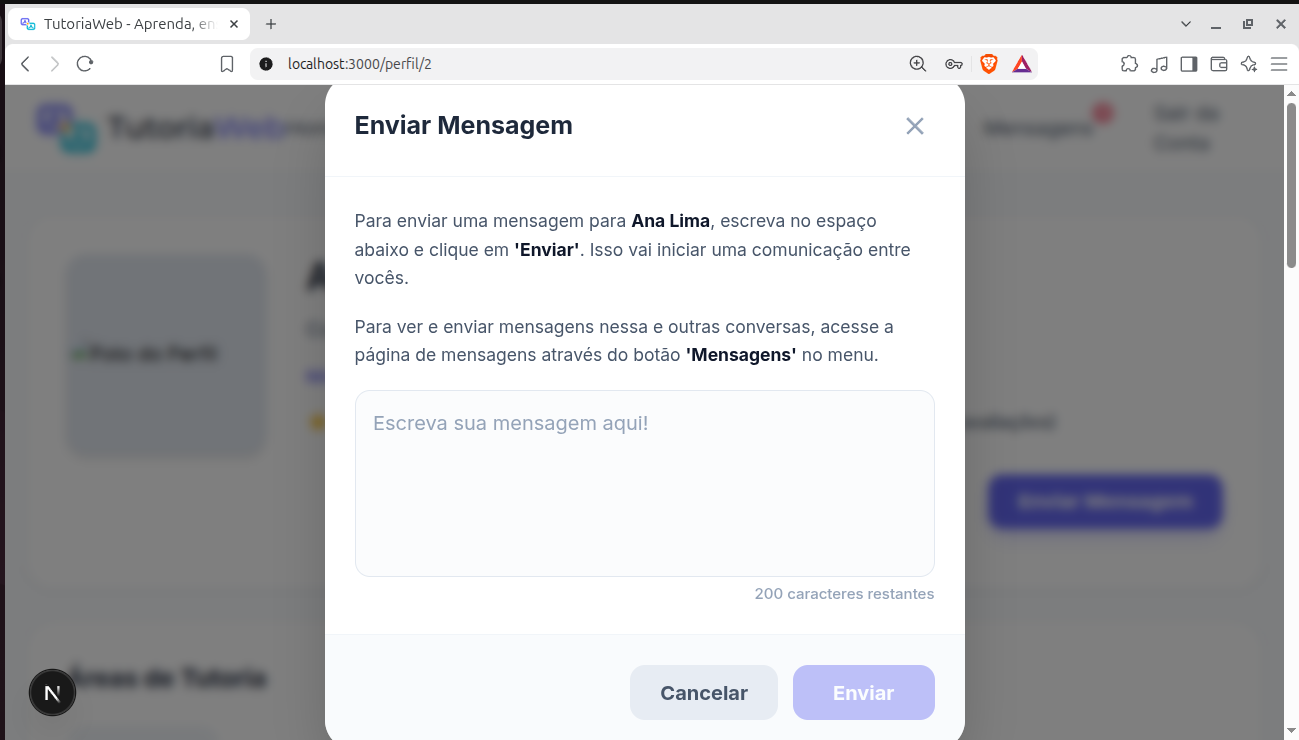
\includegraphics[width=1.9\textwidth, height=0.90\textheight, keepaspectratio]{figuras/modalMensagens.png}
    
        Fonte: Autoria própria.
        
        \vspace{0.2cm}
            
        \label{fig:modalMensagens}
    \end{figure}
\end{landscape}
\clearpage

\begin{landscape}
    \setlength{\oddsidemargin}{\evensidemargin}
    \numeracaoPaisagem
    \begin{figure}[H]
        \centering
        \caption{Página e histórico de mensagens.}
        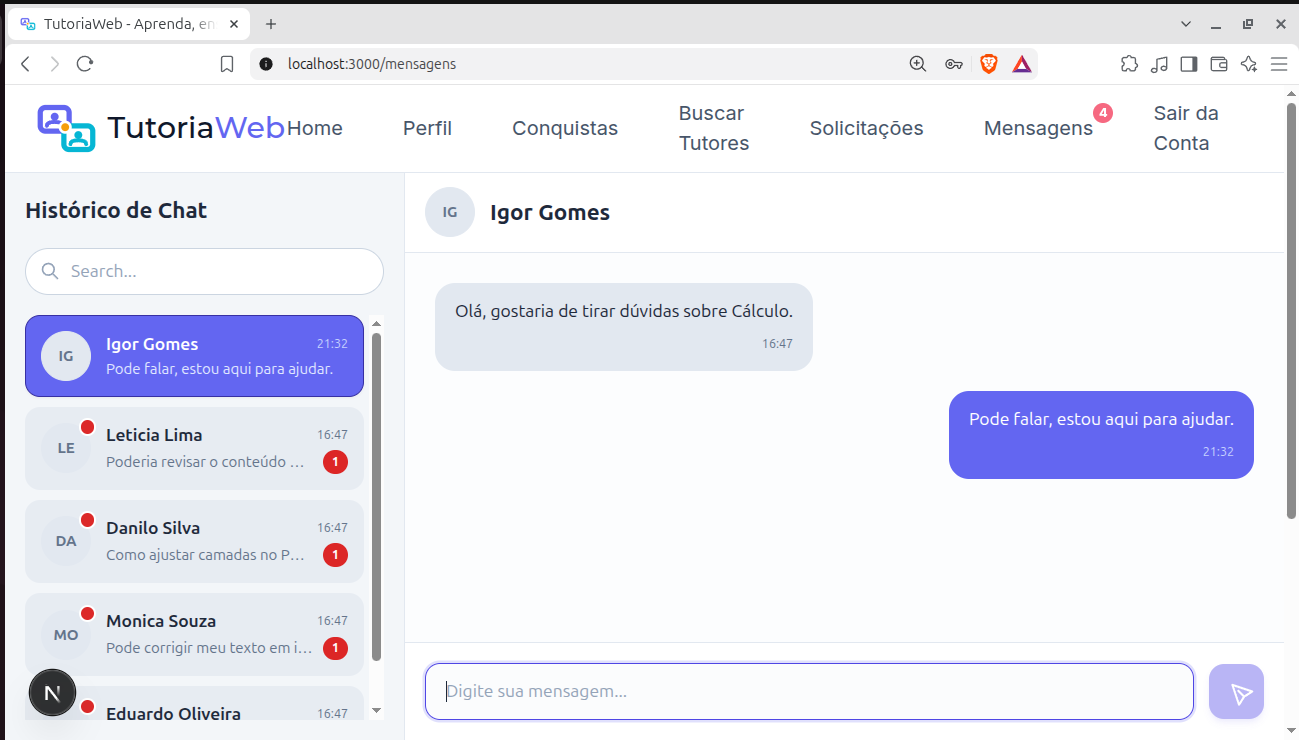
\includegraphics[width=1.9\textwidth, height=0.90\textheight, keepaspectratio]{figuras/janelaMensagens.png}
    
        Fonte: Autoria própria.
        
        \vspace{0.2cm}
            
        \label{fig:janelaMensagens}
    \end{figure}
\end{landscape}
\clearpage

\subsection[Funcionalidade 6: Busca e Recomendação de Tutores]{Funcionalidade 6: Busca e Recomendação de Tutores}

\subsubsection[US14: Buscar Tutores]{US14: Buscar Tutores}

A estimativa inicial para o desenvolvimento dessa US era na Semana 6, de 12 a 18 de abril. O desenvolvimento do \textit{backend} ocorreu do dia 18 de março, havendo refatorações na \textit{view} de Tutor para paginação e outras modificações do dia 25 até o dia 29 de maio, e mais uma modificação nos dia 18 e 20 de julho a respeito de adição de atributos de ordenação. O desenvolvimento do \textit{frontend} começou no dia 5 de maio com a criação da página de busca de tutores, sendo pausado até 25 de maio, data em que foi realizada a integração com o \textit{backend}. Em 1 de junho foi realizada a paginação dos resultados, sendo o desenvolvimento pausado novamente até o dia 18 de junho, data em que foi implementada as ordenações dos resultados por nota média de avaliação dos tutores e por quantidade de tutorias realizadas. O \textit{frontend} foi finalizado em 12 de agosto, com a adição do filtro por raio de distância.

A página de busca de tutores apresenta inicialmente apenas as opções de filtros e ordenações. Quando o usuário clica no botão ``Pesquisar'', é feita uma requisição ao \textit{backend} que retorna os tutores que atendem aos critérios definidos nos filtros. Caso nenhum filtro tenha sido definido, os tutores são retornados de acordo com a ordem dos registros no banco de dados. Os resultados são páginados e a quantidade de tutores por página podem ser alterados entre 6, 12, e 18. Caso nenhum tutor tenha sido encontrado, um texto informativo é exibido. A página com resultados pode ser observada na Figura \ref{fig:paginaBuscaTutores}.

Cada tutor é exibido em um \textit{card}, que exibe seu nome, foto, localização, nota média de avaliação (juntamente com a quantidade de avaliações) e as áreas de conhecimento que o mesmo fornece tutorias. Ao se clicar no botão ``Ver Perfil'', o usuário é redirecionado ao perfil do tutor, onde pode realizara as interações já mencionadas anteriormente (solicitar sessão e enviar mensagem).

Uma melhoria realizada durante o desenvolvimento dessa US foi a possibilidade de, além da filtragem dos resultados por área de conhecimento, ser feita a filtragem por especialidade nessa área, tornando a busca mais precisa.

Não houveram dificuldades no desenvolvimento ambas as frentes desta US.

\begin{landscape}
    \setlength{\oddsidemargin}{\evensidemargin}
    \numeracaoPaisagem
    \begin{figure}[H]
        \centering
        \caption{Página de busca de tutores com resultados.}
        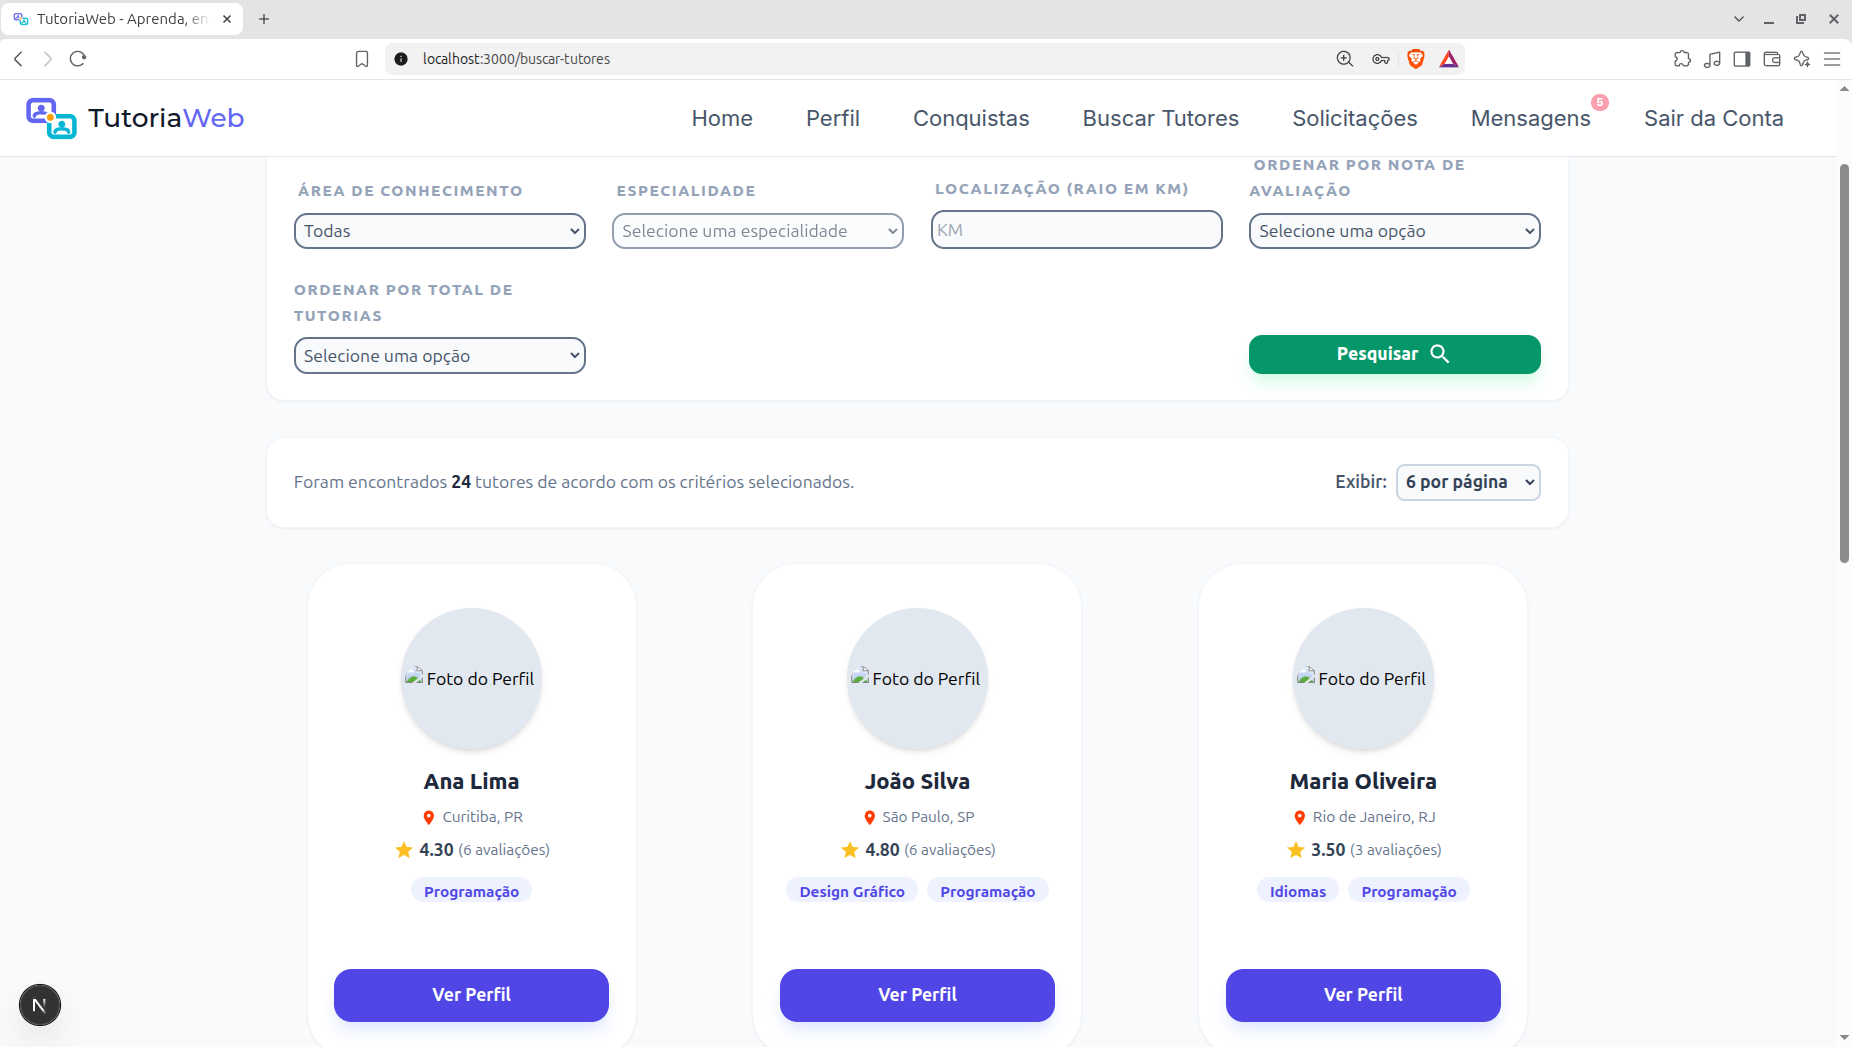
\includegraphics[width=1.9\textwidth, height=0.90\textheight, keepaspectratio]{figuras/paginaBuscaTutores.png}
    
        Fonte: Autoria própria.
        
        \vspace{0.2cm}
            
        \label{fig:paginaBuscaTutores}
    \end{figure}
\end{landscape}
\clearpage

\subsubsection[US15: Recomendações]{US15: Recomendações}

A estimativa inicial para o desenvolvimento dessa US era na Semana 10, de 10 a 16 de maio. O desenvolvimento do \textit{backend} foi realizado do dia 20 à 26 de maio, havendo modificações de parâmetros futuros nos dias 20 de julho, 20 de agosto e 18 de setembro. O desenvolvimento \textit{frontend} foi adiantado para o dia 5 de maio, juntamente com a página de busca de tutores. Isso ocorreu pois ambas as páginas são muito parecidas, então aproveitou-se grande parte do código da página de busca de tutores. O desenvolvimento foi pausado até o dia 20 de agosto, onde foi realizada a integração com o \textit{backend}.

A solução para o sistema de recomendação executa uma requisição em um \textit{endpoint GET}, o qual executa o sistema de recomendação hibrído proposto pelos autores. Este sistema utiliza bibliotecas matemáticas avançadas do Python:

\begin{itemize}
    \item \textbf{Pandas e Numpy:} Usados para a criação de \textit{DataFrames} (estruturas de tabelas tabulares) e operações matemáticas vetoriais;
    \item \textbf{Scikit-learn:} Emprega o método \textit{cosine\_similarity} para calcular distâncias entre vetores, e \texttt{MultiLabelBinarizer} para realizar a transformação \textit{One-Hot Encoding} (binarização de classes textuais/id) das especialidades.
\end{itemize}

O algoritmo busca tutores usando filtros baseados nos parâmetros fornecidos na URL:

\begin{itemize}
    \item \textbf{Área:} É obrigatório fornecer pelo menos a área de conhecimento que se deseja uma tutoria;
    \item \textbf{Especialidade:} A especialidade, caso enviada, tem prevalência sobre a área;
    \item \textbf{Geolocalização:} Se um \texttt{raio} for fornecido, a distância em quilômetros é conferida. O código traz suporte nativo ao PostGIS (\textit{distance\_lte}) e inclui um método de tolerância (\textit{fallback}) por cálculo de \textit{Haversine} via código puramente matemático, caso não haja extensão espacial no banco de dados.
\end{itemize}

Após reduzir o número de tutores na consulta ao banco, as informações dos tutores restantes são processadas em massa e montadas em um dicionário focado nas especialidades (\texttt{tutor\_specs\_map}), que finalmente se transforma no \textit{DataFrame} \texttt{df\_tutors}.

Depois começa-se a etapa de filtragem baseada em conteúdo. Esta etapa calcula se o perfil intrínseco do tutor satisfaz os interesses do usuário:
\begin{itemize}
    \item O sistema monta um vetor de interesse partindo do zero. O interesse do usuário ``aumenta'' (ganha \textit{boosts}) conforme ações declaradas: receber peso +10.0 se solicitou a especialidade exata, e +2.0 em todos os subtópicos se pediu apenas a área;
    \item O motor consulta o histórico passado de sessões, atribuindo bônus adicionais caso ele já tenha cursado especialidades específicas;
    \item A \textbf{Similaridade de Cosseno} cruza esse vetor de interesse com as características \textit{One-Hot} do tutor, gerando uma nota inicial (\texttt{content\_score}). Ela ainda recebe um incremento caso o tutor resida na mesma cidade (+3.0) ou estado (+1.0), além de bônus atrelados às pontuações nativas da aplicação.
\end{itemize}

Logo após essa etapa inicia-se a filtragem colaborativa, em que a lógica infere a nota que o usuário daria ao tutor baseado no que usuários de perfis semelhantes pensam:
\begin{itemize}
    \item Monta-se uma \textbf{Matriz de Correlação Usuário-Item} coletando todas as avaliações (\texttt{AvaliacaoTutorModel}) na aplicação;
    \item Uma Similaridade de Cosseno identifica os "10 usuários mais parecidos" com o aluno. Realiza-se, então, uma média ponderada das avaliações desses ``vizinhos próximos'';
    \item Há tratamento de ``Início Frio`'' (\textit{Cold Start}): se for um usuário recém-criado, a predição adota a média universal daquele tutor.
\end{itemize}

Para a unificação das duas etapas, o \textit{score} colaborativo possui peso maior em comparação ao de conteúdo. A nota definitiva (\texttt{final\_score}) se torna igual ao dobro da nota colaborativa somada ao da nota de conteúdo.

Por último, o algoritmo reordena o \textit{DataFrame} de forma decrescente, remapeia essas notas matemáticas (\textit{final\_score}) dinamicamente na classe \textit{TutorModel} como a propriedade virtual \textit{.score}, e envia a lista ordenada ao paginador \textit{RecomendacaoPagination} e respectivo serializador JSON.

A página de recomendações é acessada clicando-se no botão ``Ver Recomendações'' na página de busca de tutores. Conforme mencionado, essa página é bastante similar à página de busca de tutores

Conforme citado, a página de recomendação de tutores é bastante similar à página de busca de tutores, contendo, entretanto, apenas filtragem por área de conhecimento (que é obrigatória), especialidade e por localização dentro de um raio de distância em quilômetros a partir da localização do usuário.

Os resultados são exibidos da mesma maneira que na página de busca de tutores: paginados e com cada tutor sendo exibido em um \textit{card}, que contém as mesmas informações já mencionadas anteriormente e o botão que leva o usuário para o perfil do tutor. A página com resultados pode ser observada na Figura \ref{fig:paginaRecomendacoes}.

Houve uma mudança nessa funcionalidade durante o desenvolvimento. Inicialmente, a ideia era que o usuário informasse em seu perfil as áreas que possui interesse em receber tutoria, conforme o CA01. Entretanto, os autores notaram que isso prejudicava a experiência do usuário, visto que o usuário teria que adicionar áreas no perfil para obter recomendações, e deletar áreas de interesse para deixar de recebê-las. Ao se remover as áreas de interesse e centralizar toda a funcionalidade de recomendações em uma única página, esta etapa intermediária de gerenciamento no perfil deixou de existir, melhorando a funcionalidade.

O desenvolvimento desta funcionalidade no \textit{backend} apresentou obstáculos técnicos significativos, exigindo uma extensa curva de aprendizado sobre a arquitetura de um SR. Devido à complexidade matemática e de engenharia de dados do tema, foi necessário destinar mais de uma \textit{sprint} exclusivamente para o estudo teórico e o planejamento da implementação desta US. Os autores dedicaram-se a pesquisar aprofundadamente o funcionamento das bibliotecas \textit{Pandas}, \textit{NumPy} e \textit{Scikit-learn} para dominar e viabilizar as operações vetoriais e a manipulação de dados. Além da curva de aprendizado com as novas ferramentas, foi imprescindível uma investigação minuciosa sobre filtragem colaborativa e baseada em conteúdo, a fim de compreender de fato as metodologias de cálculo de similaridade e como integrar e ponderar essas lógicas na construção de um algoritmo híbrido otimizado.

Não houveram dificuldades no desenvolvimento do \textit{frontend}.

\begin{landscape}
    \setlength{\oddsidemargin}{\evensidemargin}
    \numeracaoPaisagem
    \begin{figure}[H]
        \centering
        \caption{Página de busca de tutores com resultados.}
        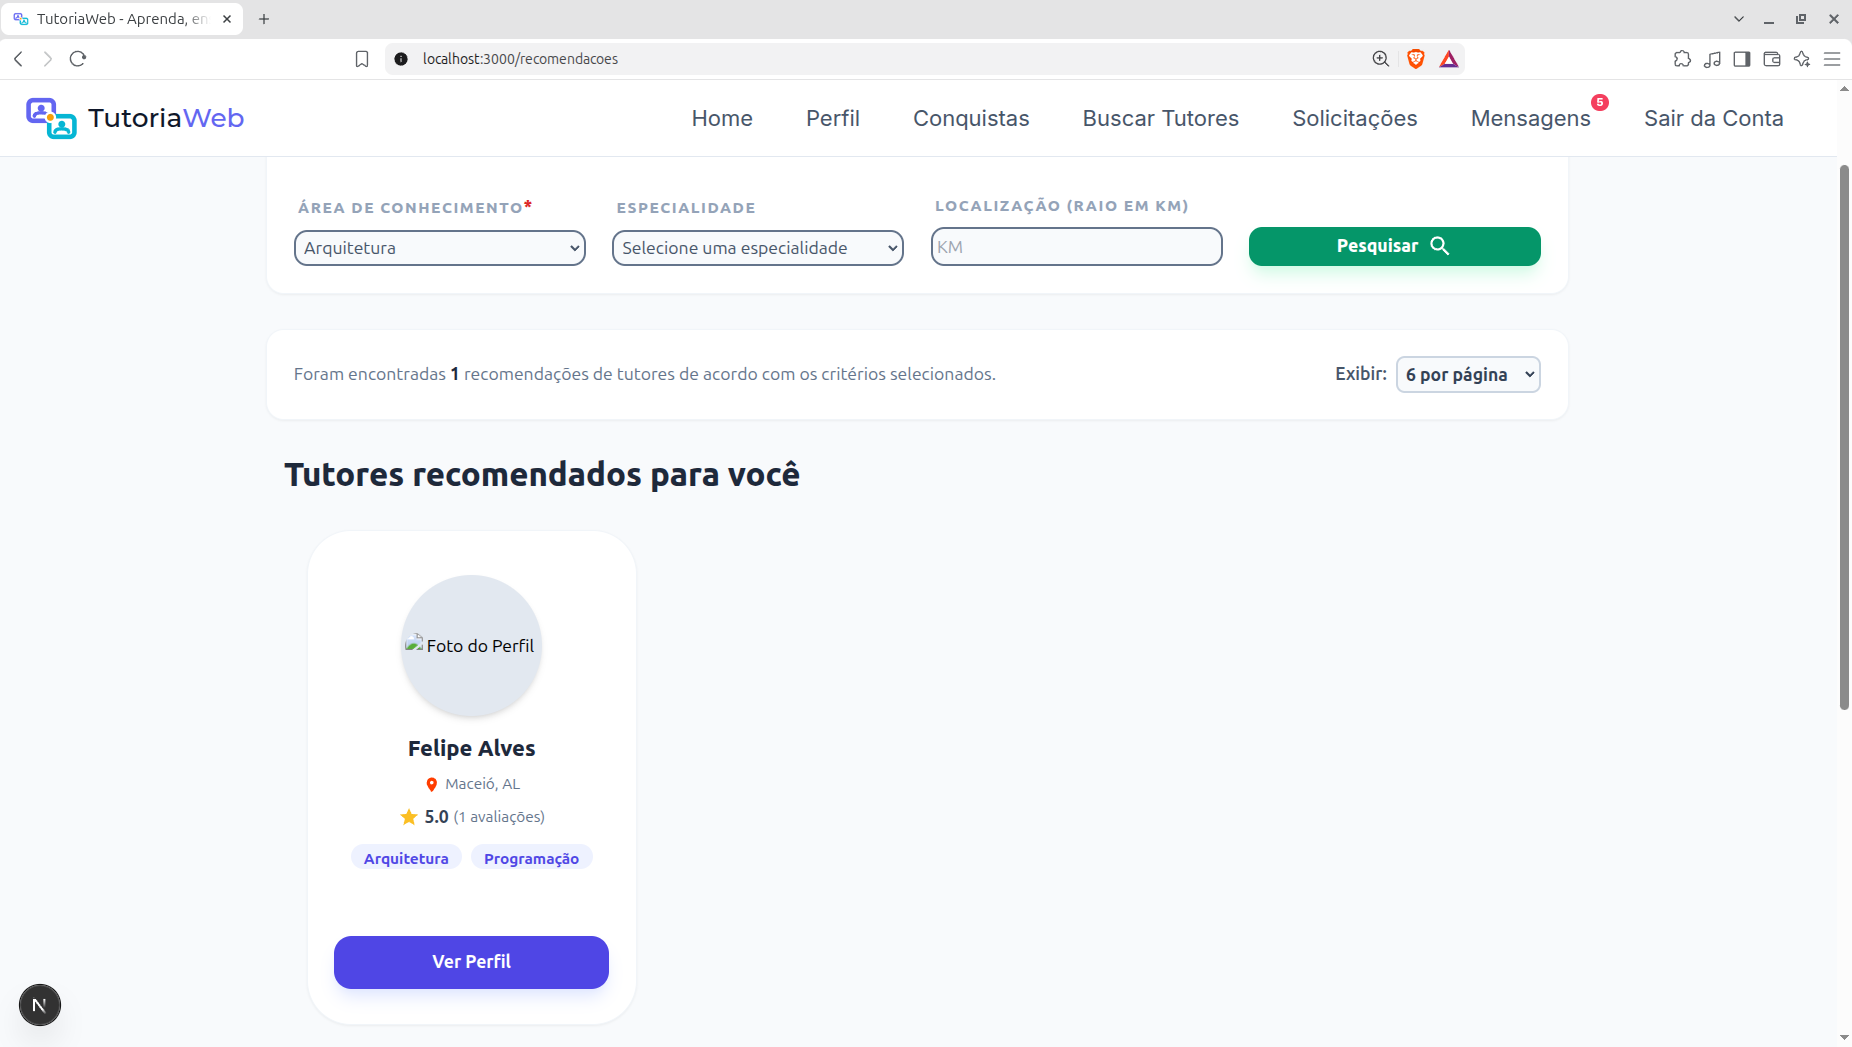
\includegraphics[width=1.9\textwidth, height=0.90\textheight, keepaspectratio]{figuras/paginaRecomendacoes.png}
    
        Fonte: Autoria própria.
        
        \vspace{0.2cm}
            
        \label{fig:paginaRecomendacoes}
    \end{figure}
\end{landscape}
\clearpage

\subsection[Funcionalidade 7: Sistema de Gamificação]{Funcionalidade 7: Sistema de Gamificação}

\subsubsection[US16: Conquistas]{US16: Conquistas}

A estimativa inicial para o desenvolvimento dessa US era na Semana 11, de 17 a 23 de maio. O desenvolvimento do \textit{frontend} começou em 28 de agosto, sendo pausado até 10 de setembro e terminado em 19 de setembro. O \textit{backend} foi completamente reutilizado da simulação, feito nos dias 20 e 23 de outubro, apenas recebendo alterações em \textit{endpoints GET} no dia 11 de setembro por conta de mudanças na tabela de conquistas no banco de dados, conforme será explicado mais adiante.

O desenvolvimento do \textit{frontend} começou com a página de conquistas e os \textit{cards} delas, mas foi pausado pois foi necessário gerar as imagens que serviriam de ícones no card. As imagens foram geradas por \textit{prompts} no Google Gemini, um \textit{chatbot} de inteligência artificial da Google. Esse processo foi demorado devido à quantidade considerável de conquistas, sendo 31 ao todo. Além disso, por vezes foi necessário repetir ou refinar os \textit{prompts} para se obter um resultado satisfatório.

Após todas as imagens serem geradas e redimensionadas para uma resolução menor, o desenvolvimento foi retomado, sendo implementado o evento de desbloqueio das conquistas, bem como uma notificação visual para quando esse evento ocorre, que é acompanhado de um efeito sonoro tocado pelo navegador. A página de conquistas e a notificação podem ser observadas nas Figuras \ref{fig:paginaConquistas} e \ref{fig:notificacaoConquista}.

Os autores buscaram diversificar os objetivos das conquistas, buscando envolver todas as atividades possíveis dentro da aplicação e tanto no papel de tutor como no papel de aprendiz. Como exemplos, pode-se citar conquistas cujo desbloqueio são enviar mensagem para tutores, conseguir alcançar determinados níveis, conseguir uma avaliação nota 5 como tutor e aprendiz e realizar um determinado número de sessões.

Duas evoluções que os autores pensaram e implementaram para essa US durante o desenvolvimento foram a criação de classificações para as conquistas, cujo critério é a dificuldade de sua obtenção, e a criação de conquistas secretas, cujos \textit{cards}, diferentes das outras conquistas, não possui uma descrição do que deve ser feito para serem obtidas, e sim uma pista sugestiva. Quando são desbloquadas, o \textit{card} se torna o de uma conquista normal, exibindo o título, classificação, pontuação e descrição. \textit{Cards} de conquistas secretas podem ser observados na Figura \ref{fig:conquistaSecreta}.

A classificação de conquistas foi implementada inspirada no sistema de troféus do PlayStation 3, em que cada conquista, representada por um troféu, é classificada como bronze, prata, ouro ou platina. Essas categorias foram utilizadas na aplicação, apenas trocando-se platina por diamante. Essa ideia é embasada pelos \textit{Core Drives} de Yu-Kai Chou mencionados na Subseção \ref{sec:gamificacao}.

Ter categorias de conquistas ativa a natureza colecionadora do usuário, incentivando o comportamento de tentar obter a coleção inteira das categorias mais difíceis. Isso é um aplicação do \textit{Core Drive} de Propriedade e Posse. A mudança também é justificada pelo \textit{Core Drive} de Desenvolvimento e Realização. A classificação tangibiliza o esforço do usuário. Uma conquista de categoria ouro ou diamante ser desbloqueada comunica que um objetivo difícil foi alcançado, trazendo uma sensação maior de realização. 

A ideia de conquistas secretas também foi inspirada no sistema do PlayStation, com a diferença de que a aplicação fornece pistas sugestivas para o usuário, algo ausente em troféus secretos. O objetivo era instigar a curiosidade do usuário e fazê-lo ter comportamentos incomuns a fim de destravá-las.

Isso é justamente o conceito do \textit{Core Drive} de Empoderamento da Criatividade e \textit{Feedback}: engajar o usuário em um processo criativo onde precisa descobrir novas estratégias. Além disso, essa mudança também é embasada pelo \textit{Core Drive} de Escassez e Impaciência: o impulso de desejar algo simplesmente porque é raro, exclusivo ou difícil de obter imediatamente. Pelo fato de serem secretas, essas conquistas se tornam mais raras de se ter, gerando um desejo de obtê-las.

\begin{landscape}
    \setlength{\oddsidemargin}{\evensidemargin}
    \numeracaoPaisagem
    \begin{figure}[H]
        \centering
        \caption{Página de conquistas.} 
        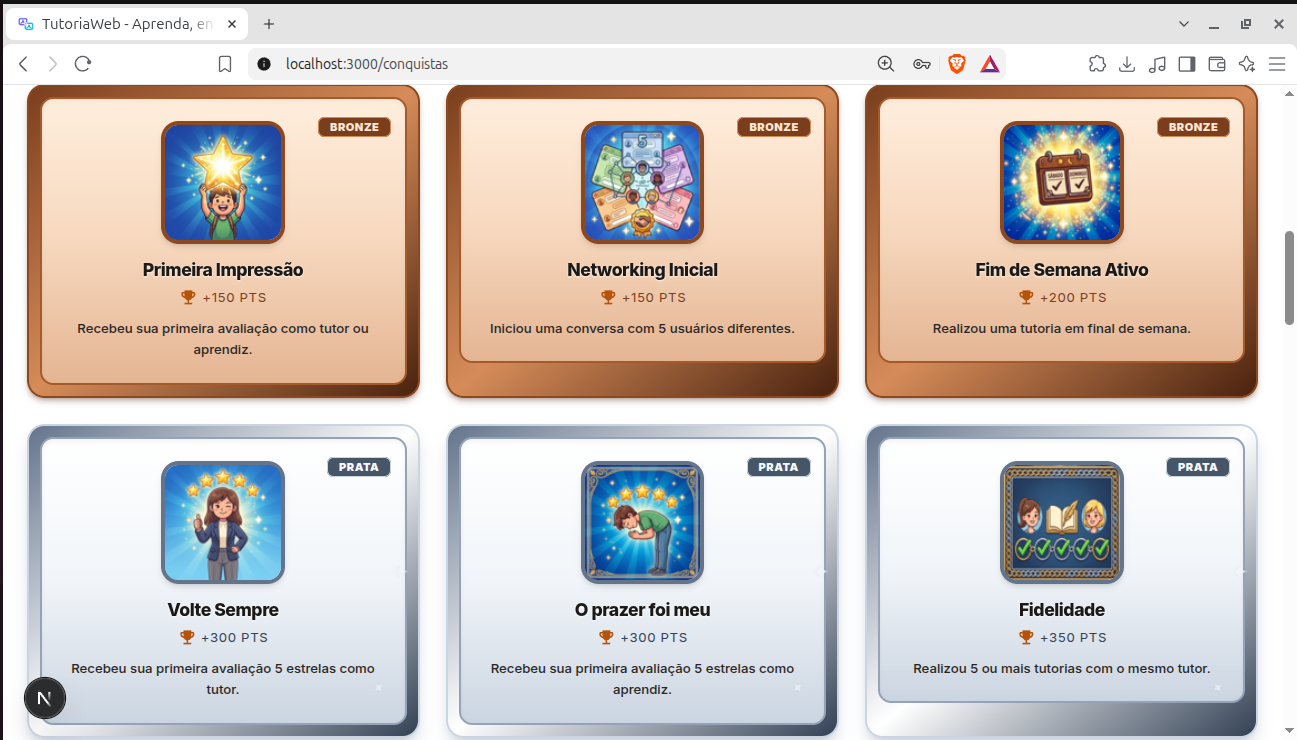
\includegraphics[width=1.9\textwidth, height=0.90\textheight, keepaspectratio]{figuras/paginaConquistas.png}
    
    
        Fonte: Autoria própria.
        
        \vspace{0.2cm}
            
        \label{fig:paginaConquistas}
    \end{figure}
\end{landscape}
\clearpage

\begin{landscape}
    \setlength{\oddsidemargin}{\evensidemargin}
    \numeracaoPaisagem
    \begin{figure}[H]
        \centering
        \caption{Notificação de conquista desbloqueda.} 
        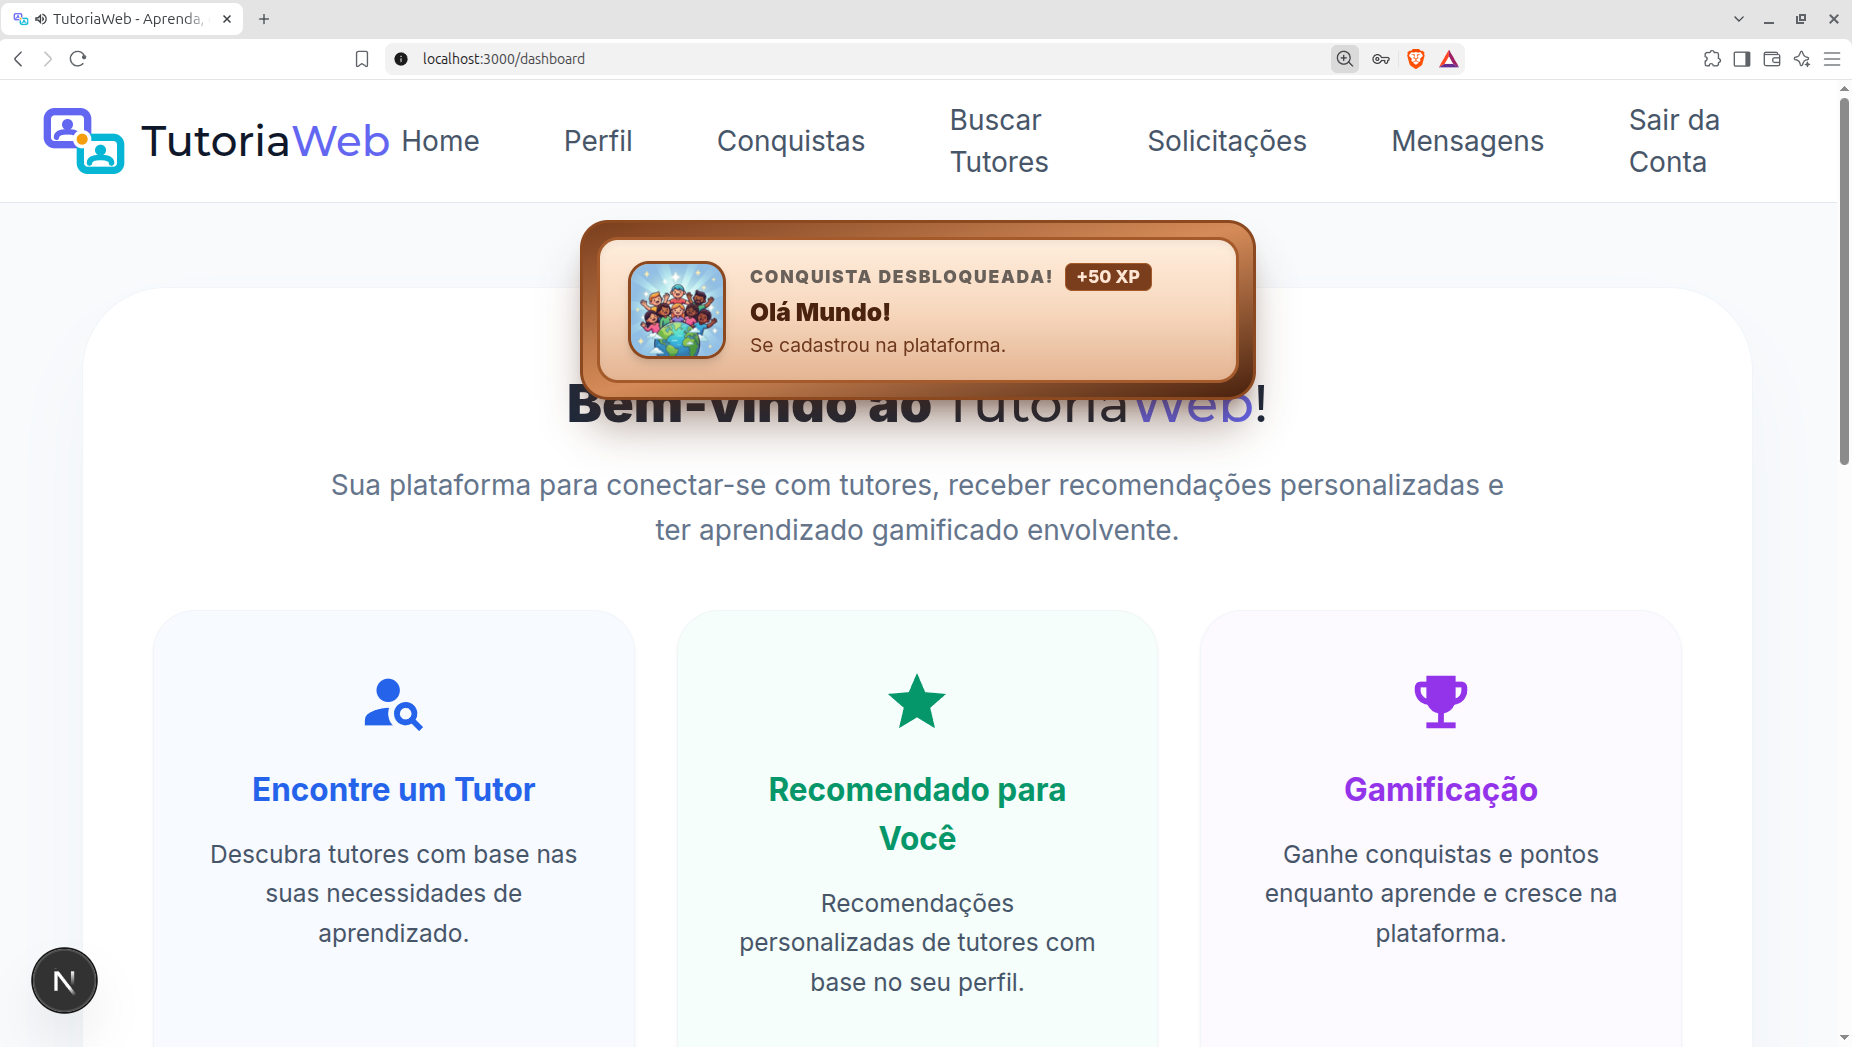
\includegraphics[width=1.9\textwidth, height=0.90\textheight, keepaspectratio]{figuras/notificacaoConquista.png}
    
    
        Fonte: Autoria própria.
        
        \vspace{0.2cm}
            
        \label{fig:notificacaoConquista}
    \end{figure}
\end{landscape}
\clearpage

\begin{landscape}
    \setlength{\oddsidemargin}{\evensidemargin}
    \numeracaoPaisagem
    \begin{figure}[H]
        \centering
        \caption{\textit{Cards} de conquistas secretas.} 
        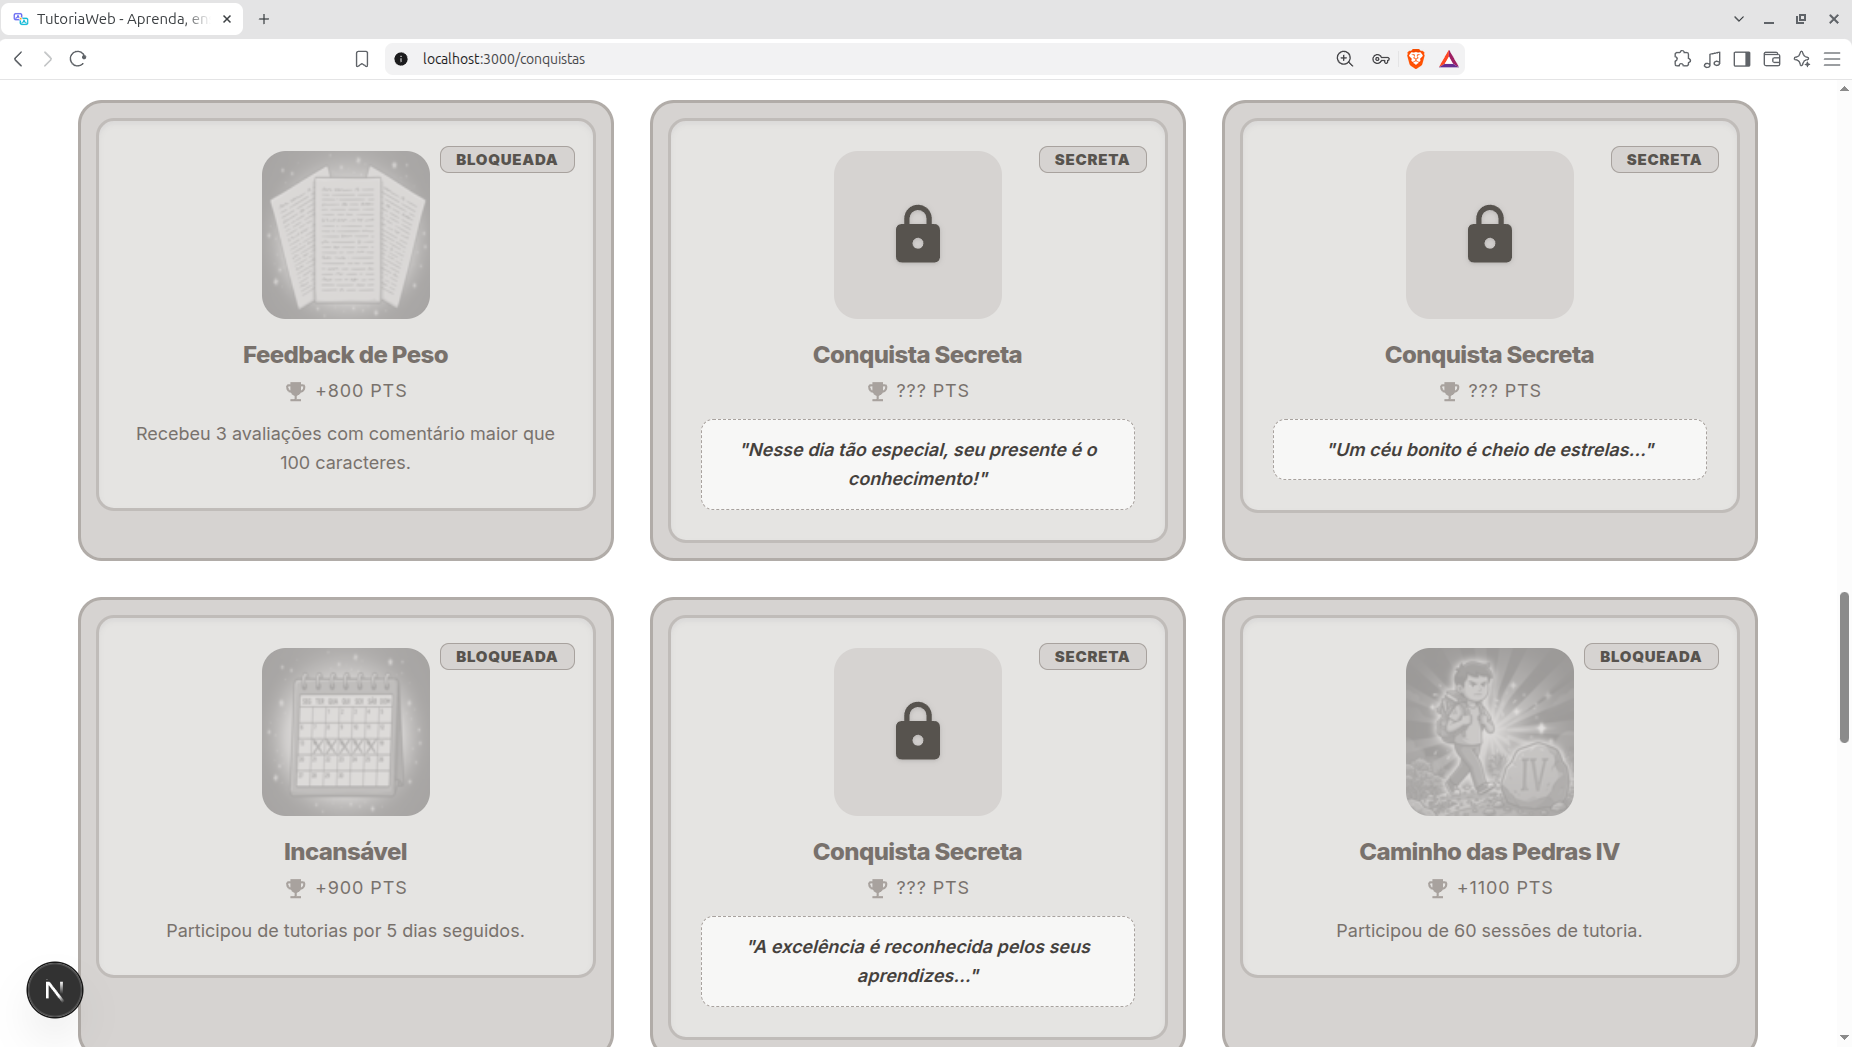
\includegraphics[width=1.9\textwidth, height=0.90\textheight, keepaspectratio]{figuras/conquistaSecreta.png}
    
    
        Fonte: Autoria própria.
        
        \vspace{0.2cm}
            
        \label{fig:conquistaSecreta}
    \end{figure}
\end{landscape}
\clearpage

Não houve dificuldades técnicas no desenvolvimento dessa US no \textit{frontend}. O maior empecilho foi a quantidade considerável de conquistas, demandando bastante tempo para a geração de todas as imagens e codificação dos gatilhos de desbloqueio na aplicação.

\subsubsection[US17: Níveis e US18: Títulos]{US17: Níveis e US18: Títulos}

Essas US vão ser relatadas em conjunto por serem muito curtas, não havendo necessidade de uma subseção inteira apenas para elas, e também por serem intrínsecamente relacionadas.

A estimativa inicial para o desenvolvimento delas era na Semana 12, de 24 a 30 de maio. Entretanto, foram adiantadas para 3 de abril, sendo as duas concluídas nessa data. O motivo do adiantamento é devido à página de perfil exibir o nível e o título decoraritivo do usuário. Sendo assim, quando a página estava sendo desenvolvida, essas US foram feitas antecipadamente a fim de se completá-la totalmente.

Essas duas funcionalidades não tiveram nenhum desenvolvimento no \textit{backend}, sendo feitas inteiramente no \textit{frontend}. Foi criado um arquivo que contém os limites de pontos de cada nível, com valores que determinam a faixa de pontuação de cada nível. Esse arquivo foi posteriormente refatorado em 7 de setembro pois os valores iniciais dificultavam demasiadamente a obtenção de níveis mais altos. Além dos limites, o arquivo também contém uma função que recebe uma pontuação e retorna qual é o nível correspondente à ela.

Os títulos foram criados em um arquivo separado, que contém uma lista dos pares de níveis e títulos correspondentes e também uma função que recebe um nível e retorna o título equivalente a ele. Dessa maneira, quando os dados de um usuário são obtidos na página do perfil dele, a função de nível retorna o nível do usuário de acordo com sua pontuação, e o retorno dela usado como parâmetro da função de título. O resultado de ambas as funções é exibido na página. A relação entre as faixas de pontuação, nível e título pode ser observada na Tabela \ref{tab:niveis-titulos}.

Não houveram dificuldades no desenvolvimento dessas US.

\newpage

\begin{table}
    \centering
    \caption{Relação entre faixas de pontuação, níveis e títulos.}
    \label{tab:niveis-titulos}
    % Mudança aqui: de tabularx{\linewidth} para tabular
    \begin{tabular}{|l|l|l|}
        \hline
        \textbf{Faixa de Pontuação} & \textbf{Nível} & \textbf{Título} \\
        \hline
        0 -- 100 & 1 & NPC Genérico 
        \\
        \hline
        101 -- 250 & 2 & Noob com Orgulho
        \\
        \hline
        251 -- 450 & 3 & Sobrevivi ao Tutorial
        \\
        \hline
        451 -- 700 & 4 & Genin Esforçado
        \\
        \hline
        701 -- 2.700 & 5 a 9 & Jovem Padawan
        \\
        \hline
        2.701 -- 5.950 & 10 a 14 & Farmador de XP
        \\
        \hline
        5.951 -- 10.450 & 15 a 19 & Estagiário Sênior
        \\
        \hline
        10.451 -- 16.200 & 20 a 24 & Faixa Preta de Taubaté 
        \\
        \hline
        16.201 -- 23.200 & 25 a 29 & Caçador de Conquistas 
        \\
        \hline
        23.201 -- 31.450 & 30 a 34 & O miserável é um gênio!
        \\
        \hline
        31.451 -- 40.950 & 35 a 39 & Super Saiyajin Base
        \\
        \hline
        40.951 -- 51.700 & 40 a 44 & Sábio dos Seis Caminhos
        \\
        \hline
        51.701 -- 63.700 & 45 a 49 & Speedrunner do Saber 
        \\
        \hline
        63.701 ou mais & 50 & Platina Humana  
        \\
        \hline
    \end{tabular}
    \vspace{0.2cm} % Um pequeno espaço antes da fonte
    
    Fonte: Autoria Própria.
\end{table}

\section[Mudanças no banco de dados]{Mudanças no banco de dados}

O banco de dados inicialmente planejado para a aplicação passou por alterações durante o desenvolvimento das funcionalidades para melhor adequação às funcionalidades ou para realização de melhorias. Essas mudanças foram mencionadas nas subseções das US, mas para melhor visualização da estrutura final, o DLD foi refeito, podendo ser observado na Figura \ref{fig:DLD_novo}. Para melhor visualização, o arquivo de imagem do DE-R pode ser acessado por este \textit{link}: \url{https://github.com/TutoriaWebApp/TCC/blob/main/overleaf/figuras/DLD_tcc2v2.png}.

O Dicionário de Dados também foi atualizado para incluir essas alterações, apresentando-as em mais detalhes e podendo ser lido no Apêndice \ref{dicionario-dados}.

\begin{landscape}
    \setlength{\oddsidemargin}{\evensidemargin}
    \numeracaoPaisagem
    \begin{figure}[H]
        \centering
        \caption{DLD atualizado.} 
        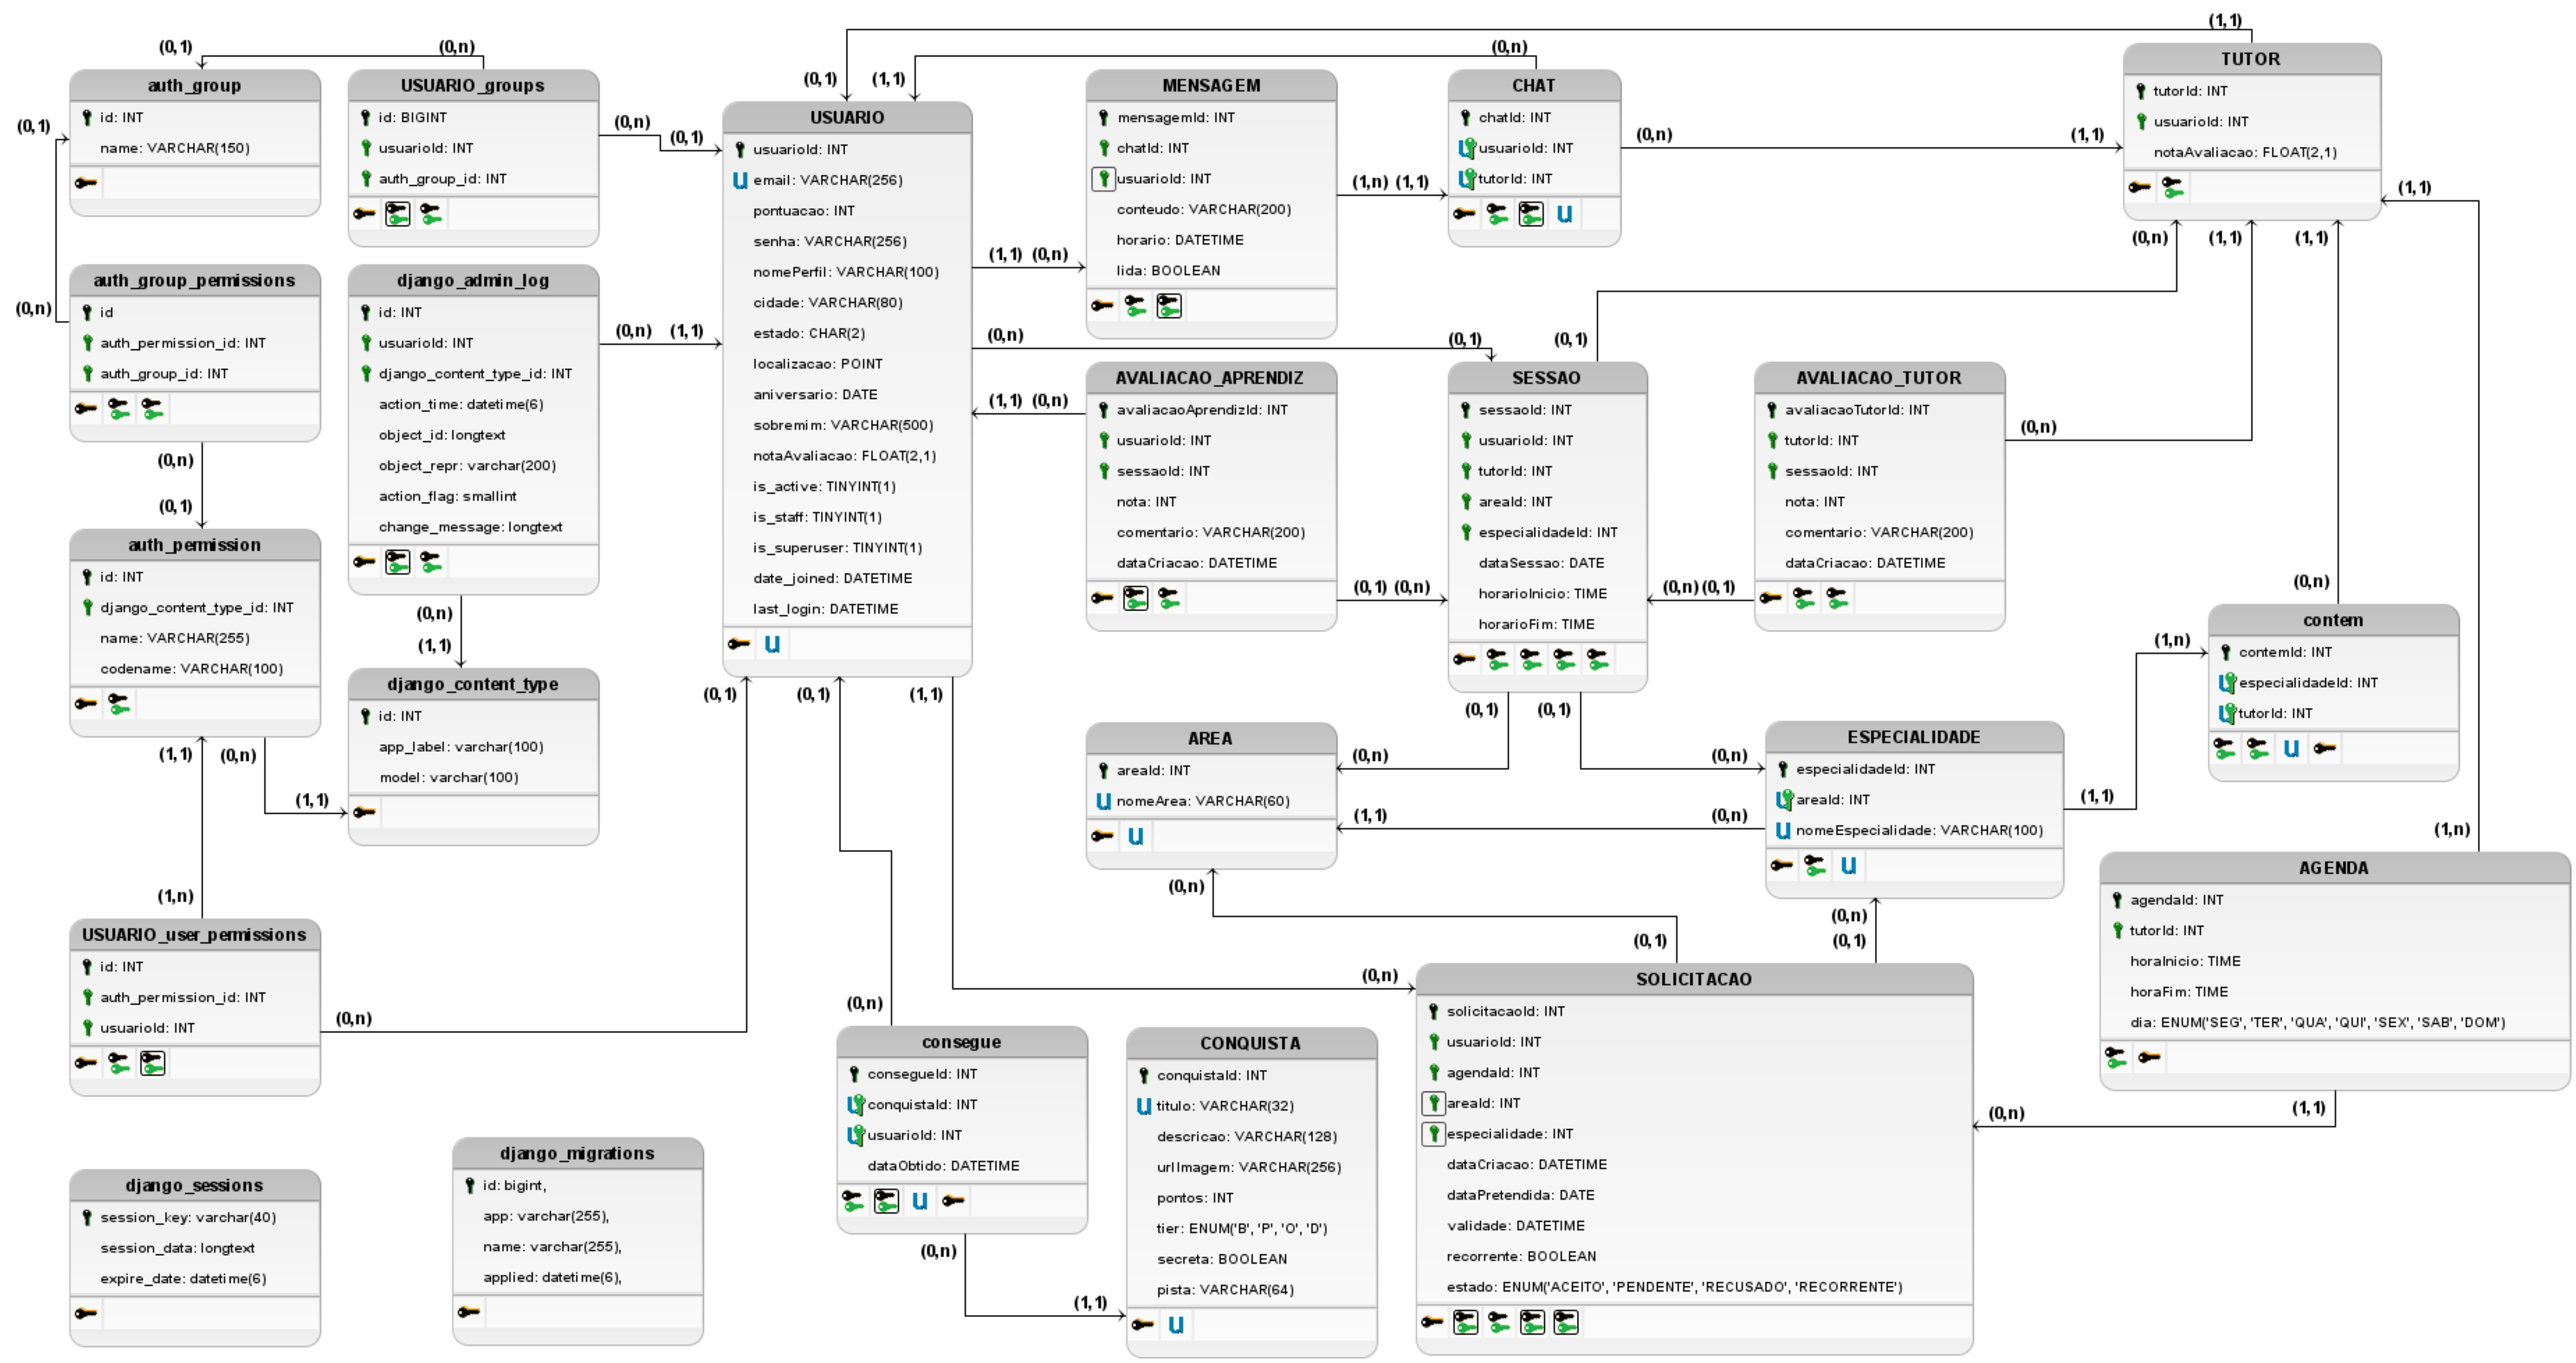
\includegraphics[width=1.9\textwidth, height=0.90\textheight, keepaspectratio]{figuras/DLD_tcc2v2.png}
    
    
        Fonte: Autoria própria.
        
        \vspace{0.2cm}
            
        \label{fig:DLD_novo}
    \end{figure}
\end{landscape}
\clearpage

\section[Teste de Software]{Teste de Software}

Conforme a Subseção \ref{sec:PlanoDeTestes}, a estratégia de testes para a aplicação proposta consistiu na implementação de testes unitários, de integração e E2E. Essa prática garantiu que novas atualizações ou adições de funcionalidades não quebrariam as regras de negócio já consolidadas, proporcionando um ambiente seguro para o crescimento contínuo do software.

\subsection[Testes Unitários]{Testes Unitários}

Para o desenvolvimento dos testes unitários foram utilizadas ferramentas nativas do DRF, como, por exemplo, ``TestCase'', ``AP`TestCase'' e ```TestCase''. Além destas ferramentas também foi utilizado o pacote ``TestCase'' para gerar o relatório de todos os testes executados.

Os testes desenvolvidos cobriram as principais camadas da arquitetura do sistema, englobando as lógicas do modelo de banco de dados (\textit{Models}), regras de roteamento e requisições HTTP (\textit{Views} e \textit{ViewSet}), serialização de dados (\textit{Serializers}) e utilitários (\textit{Utils}).

Conforme os dados gerados pelo relatório de cobertura de testes, que podem ser observado na Tabela \ref{tab:coverageUnit}, a aplicação atingiu um índice global de \textbf{88\%} de cobertura de código, abrangendo um total de 3.367 linhas lógicas (\textit{statements}), superando os 75\% que haviam sido estabelecidos como meta.

Destaca-se que partes críticas do sistema mantiveram índices de aprovação, como por exemplo, os testes desenvolvidos para as classes de entidade (como \textit{UsuarioModelTest}, \textit{AvaliacaoModelTest}, \textit{ChatModelTest} e \textit{SessaoSolicitacaoModelTest}) e para as regras de serialização alcançaram, em sua grande maioria, \textbf{100\%} de cobertura.

As taxas de cobertura reduzidas em arquivos específicos, como certas \textit{Views} ou gerenciadores de configuração, representam trechos de código com tratamentos de exceções isoladas ou rotinas secundárias que não foram invocadas diretamente durante o ambiente simulado. Contudo, o alto percentual geral obtido (88\%) evidencia a robustez arquitetural da aplicação e garante que os fluxos principais de agendamento de sessões, gamificação (conquistas) e interação entre tutor e aprendiz funcionam conforme o planejado.

\begin{landscape}
    \setlength{\oddsidemargin}{\evensidemargin}
    \iniciarCabecalhoTabelaPaisagem
\begin{longtable}{lcccc}
\caption{Relatório da cobertura de testes.\label{tab:coverageUnit}} \\
\toprule
\textbf{Arquivo / Módulo} & \textbf{Instruções} & \textbf{Faltantes} & \textbf{Excluídos} & \textbf{Cobertura (\%)} \\
\midrule
\endfirsthead
\multicolumn{5}{c}{{\bfseries Continuação da Tabela \ref{tab:coverageUnit}}} \\
\toprule
\textbf{Arquivo / Módulo} & \textbf{Instruções} & \textbf{Faltantes} & \textbf{Excluídos} & \textbf{Cobertura (\%)} \\
\midrule
\endhead
\bottomrule
\endfoot
    config/\_\_init\_\_.py & 0 & 0 & 0 & 100\% \\
    config/authenticate.py & 19 & 3 & 0 & 84\% \\
    config/manager.py & 19 & 9 & 0 & 53\% \\
    config/settings.py & 52 & 9 & 0 & 83\% \\
    config/urls.py & 8 & 1 & 0 & 88\% \\
    manage.py & 11 & 2 & 0 & 82\% \\
    project/\_\_init\_\_.py & 0 & 0 & 0 & 100\% \\
    project/admin.py & 33 & 0 & 0 & 100\% \\
    project/apps.py & 6 & 0 & 0 & 100\% \\
    project/forms/UsuarioForm.py & 11 & 0 & 0 & 100\% \\
    project/forms/\_\_init\_\_.py & 1 & 0 & 0 & 100\% \\
    project/migrations/0001\_initial.py & 9 & 0 & 0 & 100\% \\
    project/migrations/\_\_init\_\_.py & 0 & 0 & 0 & 100\% \\
    project/models/AvaliacaoModel.py & 31 & 0 & 0 & 100\% \\
    project/models/ChatModel.py & 27 & 0 & 0 & 100\% \\
    project/models/ConquistaModel.py & 35 & 0 & 0 & 100\% \\
    project/models/SessaoModel.py & 61 & 1 & 0 & 98\% \\
    project/models/TutorModel.py & 44 & 0 & 0 & 100\% \\
    project/models/UsuarioModel.py & 36 & 3 & 0 & 92\% \\
    project/models/\_\_init\_\_.py & 7 & 0 & 0 & 100\% \\
    project/serializers/AvaliacaoSerializer.py & 53 & 3 & 0 & 94\% \\
    project/serializers/ChatSerializer.py & 59 & 4 & 0 & 93\% \\
    project/serializers/ConquistaSerializer.py & 14 & 0 & 0 & 100\% \\
    project/serializers/EstatisticaSerializer.py & 6 & 0 & 0 & 100\% \\
    project/serializers/NotificacoesSerializer.py & 12 & 0 & 0 & 100\% \\
    project/serializers/SessaoSerializer.py & 131 & 20 & 0 & 85\% \\
    project/serializers/SistemaRecomendacaoSerializer.py & 9 & 0 & 0 & 100\% \\
    project/serializers/TutorSerializer.py & 80 & 2 & 0 & 98\% \\
    project/serializers/UsuarioSerializer.py & 120 & 14 & 0 & 88\% \\
    project/serializers/\_\_init\_\_.py & 9 & 0 & 0 & 100\% \\
    project/signals.py & 33 & 0 & 0 & 100\% \\
    project/urls/api.py & 28 & 0 & 0 & 100\% \\
    project/utils/GeoLocalizacaoUtil.py & 90 & 40 & 0 & 56\% \\
    project/utils/UsuarioUtils.py & 31 & 2 & 0 & 94\% \\
    project/utils/\_\_init\_\_.py & 3 & 0 & 0 & 100\% \\
    project/views/AuthViewSet.py & 84 & 0 & 0 & 100\% \\
    project/views/AvaliacaoViewSet.py & 121 & 21 & 0 & 83\% \\
    project/views/ChatViewSet.py & 97 & 21 & 0 & 78\% \\
    project/views/ConquistaViewSet.py & 45 & 13 & 0 & 71\% \\
    project/views/DashboardViewSet.py & 20 & 8 & 0 & 60\% \\
    project/views/NotificacoesViewSet.py & 21 & 8 & 0 & 62\% \\
    project/views/SessaoViewSet.py & 261 & 51 & 0 & 80\% \\
    project/views/SistemaRecomendacaoViewSet.py & 144 & 43 & 0 & 70\% \\
    project/views/TutorViewSet.py & 135 & 27 & 0 & 80\% \\
    project/views/UsuarioViewSet.py & 71 & 14 & 0 & 80\% \\
    project/views/\_\_init\_\_.py & 11 & 0 & 0 & 100\% \\
    test/AuthTest.py & 129 & 0 & 0 & 100\% \\
    test/UsuarioUtilsTest.py & 62 & 0 & 0 & 100\% \\
    test/\_\_init\_\_.py & 23 & 0 & 0 & 100\% \\
    test/models/AreaEspecialidadeModelTest.py & 24 & 0 & 0 & 100\% \\
    test/models/AvaliacaoModelTest.py & 30 & 0 & 0 & 100\% \\
    test/models/ChatModelTest.py & 38 & 2 & 0 & 95\% \\
    test/models/ConquistaModelTest.py & 32 & 0 & 0 & 100\% \\
    test/models/SessaoSolicitacaoModelTest.py & 27 & 0 & 0 & 100\% \\
    test/models/TutorModelTest.py & 11 & 0 & 0 & 100\% \\
    test/models/UsuarioModelTest.py & 35 & 2 & 0 & 94\% \\
    test/models/\_\_init\_\_.py & 8 & 0 & 0 & 100\% \\
    test/serializers/AvaliacaoSerializerTest.py & 25 & 0 & 0 & 100\% \\
    test/serializers/ChatSerializerTest.py & 48 & 0 & 0 & 100\% \\
    test/serializers/ConquistaSerializerTest.py & 25 & 0 & 0 & 100\% \\
    test/serializers/SessaoSolicitacaoSerializerTest.py & 32 & 0 & 0 & 100\% \\
    test/serializers/TutorAreaSerializerTest.py & 43 & 0 & 0 & 100\% \\
    test/serializers/UsuarioSerializerTest.py & 50 & 0 & 0 & 100\% \\
    test/serializers/\_\_init\_\_.py & 7 & 0 & 0 & 100\% \\
    test/views/AvaliacaoViewSetTest.py & 77 & 0 & 0 & 100\% \\
    test/views/ChatViewSetTest.py & 65 & 0 & 0 & 100\% \\
    test/views/ConquistaViewSetTest.py & 33 & 1 & 0 & 97\% \\
    test/views/SessaoViewSetTest.py & 208 & 74 & 0 & 64\% \\
    test/views/SistemaRecomendacaoViewSetTest.py & 61 & 1 & 0 & 98\% \\
    test/views/TutorViewSetTest.py & 71 & 0 & 0 & 100\% \\
    test/views/UsuarioViewSetTest.py & 97 & 0 & 0 & 100\% \\
    test/views/\_\_init\_\_.py & 8 & 0 & 0 & 100\% \\
    \midrule
    \textbf{Total} & \textbf{3367} & \textbf{399} & \textbf{0} & \textbf{88\%} \\
    \bottomrule
\end{longtable}
\end{landscape}
\terminarCabecalhoTabelaPaisagem

\subsection[Testes de Integração]{Testes de Integração}

Para a elaboração e execução dos testes de integração foi utilizada a plataforma Postman, para a construção das coleções de requisições, em conjunto com a ferramenta de linha de comando Newman, para a execução automatizada e geração do relatório.

Os testes desenvolvidos abrangeram as principais rotas da API da aplicação, simulando fluxos práticos de interação do usuário e englobando funcionalidades de autenticação (\textit{Login}, \textit{Log out} e Redefinição de Senha), gerenciamento de cadastros (Cadastrar Usuário e Perfil Logado), além das lógicas de negócio associadas à interação na aplicação, como fluxos de Sessão e Solicitar Sessão.

Conforme os dados gerados pelo \textit{dashboard} do relatório Newman na Figura \ref{fig:newman}, a coleção efetuou um total de 74 requisições HTTP, avaliando um total de 147 asserções (\textit{assertions}) globais. O ambiente de testes simulado também demonstrou um tempo total de execução de 16,3 segundos, com um excelente tempo médio de resposta de 145ms por requisição.

Destaca-se que partes críticas do sistema de comunicação da API mantiveram índices totais de aprovação. Por exemplo, os testes desenvolvidos para o fluxo de cadastro, listagem de usuários, obtenção e alteração do perfil logado, além da renovação de credenciais (\textit{Log in Refresh com Sucesso}), alcançaram \textbf{100\%} de aprovação em todas as suas validações.

As 15 falhas relatadas em testes específicos representam validações isoladas que não retornaram os resultados esperados, concentradas majoritariamente em verificações estritas do estado de \textit{cookies} durante falhas de \textit{login} e \textit{/log out} e no retorno de códigos HTTP divergentes (como erros 400 e 500 ao contrário dos sucessos 200 e 204) nos fluxos de aceitar, recusar e deletar solicitações de sessão. Contudo, o elevado índice geral de sucesso nas requisições demonstra a consistência arquitetural da API e garante que a integração essencial de dados, autenticação básica e listagem de informações operam com confiabilidade e solidez.

O repositório com a coleção dos testes de integração feitos no Postman e a análise do Newman podem ser acessados através desse \textit{link}: \url{https://github.com/TutoriaWebApp/Integracao}

\newpage

\begin{figure}[H]
    \centering
    \caption{Newman Summary Report.} 
    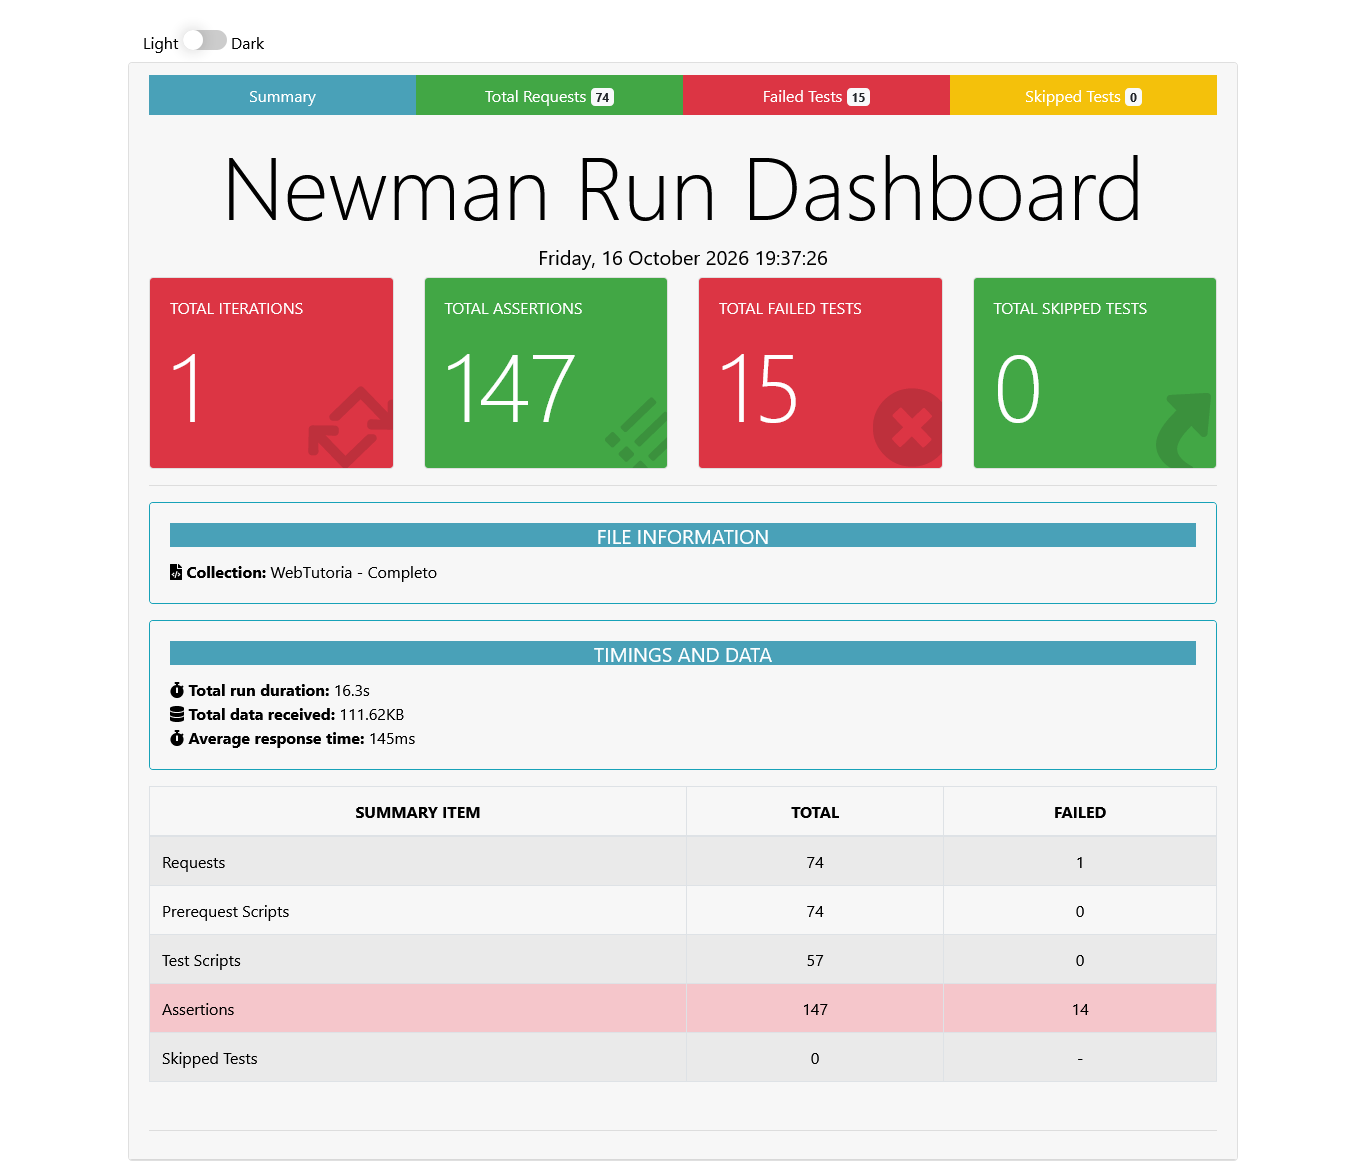
\includegraphics[width=1.1\textwidth, height=0.7\textheight, keepaspectratio]{figuras/NewmanSummaryReport.png}

    Fonte: Autoria própria.

    \vspace{0.2cm}
    
    \label{fig:newman}
\end{figure}

\subsection[Testes E2E]{Testes E2E}

Para realizar a a automação dos testes E2E da aplicação foi utilizado o \textit{framework} Robot Framework em conjunto com a biblioteca \textbf{SeleniumLibrary} e o navegador Firefox (geckodriver). A suíte de testes E2E é composta por 11 suítes funcionais integradas, englobando 38 cenários de teste que simulam fluxos completos de navegação, cadastro, autenticação, busca com geolocalização, agendamento de tutorias, troca de mensagens e gamificação.

A Tabela \ref{tab:robotE2E} apresenta o resumo quantitativo de aprovação e tempo de execução por suíte funcional. Dos 38 cenários executados, todos os 38 foram aprovados com sucesso, atingindo uma taxa de sucesso global de 100\% com tempo total de execução de aproximadamente 22,4 minutos (1.343,9 segundos).

Houveram dificuldades na realização dos testes. O Robot Framework utiliza os atributos ``id'' dos elementos HTML das páginas para permitir a seleção e interação com os mesmos. Entretanto, esses atributos estavam ausentes nas paǵinas, levando à refatorações para inclusão destes para prosseguimento dos testes.

O repositório com os arquivos utilizados nos testes pode se acessado através desse \textit{link}: \url{https://github.com/TutoriaWebApp/End2End}.

\begin{landscape}
    \setlength{\oddsidemargin}{\evensidemargin}
    \iniciarCabecalhoTabelaPaisagem
    
    \begin{longtable}{llcc}
\caption{Resultados dos cenários de teste E2E. \label{tab:robotE2E}} \\
\toprule
\textbf{Suíte} & \textbf{Cenário / Caso de Teste E2E} & \textbf{Status} & \textbf{Duração (s)} \\
\midrule
\endfirsthead
\multicolumn{4}{c}{{\bfseries Continuação da Tabela \ref{tab:robotE2E}}} \\
\toprule
\textbf{Suíte} & \textbf{Cenário / Caso de Teste E2E} & \textbf{Status} & \textbf{Duração (s)} \\
\midrule
\endhead
\bottomrule
\endfoot
01 Cadastro & Cenário: Cadastrar um novo perfil Aprendiz & \textbf{PASS} & 34.78s \\
01 Cadastro & Cenário: Cadastrar um novo perfil Tutor & \textbf{PASS} & 48.82s \\
02 Login & Cenário: Login com credenciais válidas & \textbf{PASS} & 27.67s \\
02 Login & Cenário: login com email inválido & \textbf{PASS} & 27.20s \\
02 Login & Cenário: login com senha inválida & \textbf{PASS} & 26.72s \\
03 Meu Perfil & Cenário: Visualizar Meu Perfil & \textbf{PASS} & 33.15s \\
03 Meu Perfil & Cenário: Alterar Senha & \textbf{PASS} & 39.82s \\
03 Meu Perfil & Cenário: Editar todo Perfil & \textbf{PASS} & 64.86s \\
04 Redefinir Senha & Cenário: Esqueci minha senha & \textbf{PASS} & 28.03s \\
04 Redefinir Senha & Cenário: Redefinir senha por link válido & \textbf{PASS} & 30.72s \\
04 Redefinir Senha & Cenário: Redefinir senha por link já utilizado & \textbf{PASS} & 27.80s \\
01 Buscar Tutores & Cenário: Buscar todos os tutores e verificar resultado & \textbf{PASS} & 30.91s \\
01 Buscar Tutores & Cenário: Filtrar tutores por Área de Conhecimento & \textbf{PASS} & 31.87s \\
01 Buscar Tutores & Cenário: Filtrar tutores por Área de Conhecimento e Especialidade & \textbf{PASS} & 30.30s \\
01 Buscar Tutores & Cenário: Filtrar tutores por raio de distância 1km & \textbf{PASS} & 29.22s \\
01 Buscar Tutores & Cenário: Filtrar tutores por raio de distância 1000km & \textbf{PASS} & 30.45s \\
01 Buscar Tutores & Cenário: Ordenar tutores por Nota de Avaliação de forma Decrescente & \textbf{PASS} & 29.89s \\
01 Buscar Tutores & Cenário: Ordenar tutores por Nota de Avaliação de forma Crescente & \textbf{PASS} & 30.31s \\
01 Buscar Tutores & Cenário: Ordenar tutores por Número de Sessões de forma Decrescente & \textbf{PASS} & 30.29s \\
01 Buscar Tutores & Cenário: Ordenar tutores por Número de Sessões de forma Crescente & \textbf{PASS} & 29.83s \\
02 Recomendacoes & Cenário: Visualizar tutores recomendados por Área de Conhecimento & \textbf{PASS} & 32.41s \\
02 Recomendacoes & Cenário: Visualizar tutores recomendados por Especialidade & \textbf{PASS} & 33.06s \\
02 Recomendacoes & Cenário: Visualizar tutores recomendados por Distância & \textbf{PASS} & 43.07s \\
03 Perfil Publico & Cenário: Vizualizar informações de um tutor via Buscar Tutores & \textbf{PASS} & 34.38s \\
03 Perfil Publico & Cenário: Vizualizar informações de um tutor via Recomendação & \textbf{PASS} & 36.49s \\
03 Perfil Publico & Cenário: Ver Avaliações do Tutor & \textbf{PASS} & 33.45s \\
03 Perfil Publico & Cenário: Enviar mensagem & \textbf{PASS} & 37.13s \\
03 Perfil Publico & Cenário: Visualizar informações de um tutor via link & \textbf{PASS} & 31.67s \\
03 Perfil Publico & Cenário: Solicitar tutoria a partir do perfil & \textbf{PASS} & 54.21s \\
04 Solicitacoes & Cenário: Vizualizar solicitações aceitas como Tutor & \textbf{PASS} & 30.07s \\
04 Solicitacoes & Cenário: Visualizar solicitações aceitas como Aprendiz & \textbf{PASS} & 30.12s \\
04 Solicitacoes & Cenário: Visualizar minhas solicitações & \textbf{PASS} & 29.06s \\
04 Solicitacoes & Cenário: Aceitar uma solicitação pendente & \textbf{PASS} & 39.59s \\
04 Solicitacoes & Cenário: Recusar uma solicitação pendente & \textbf{PASS} & 39.61s \\
05 Mensagens & Cenário: Sem contatos de mensagens & \textbf{PASS} & 26.94s \\
05 Mensagens & Cenário: Enviar mensagem para um contato no chat & \textbf{PASS} & 39.20s \\
06 Avaliacoes & Cenário: Avaliar sessão como Tutor e como Aprendiz & \textbf{PASS} & 61.54s \\
07 Conquistas & Cenário: Visualizar lista de conquistas e seus detalhes & \textbf{PASS} & 49.28s \\
\bottomrule
\end{longtable}
\end{landscape}
\terminarCabecalhoTabelaPaisagem

\subsection{Teste de Usabilidade}
Esta seção descreve o roteiro estruturado para a execução dos testes de usabilidade com usuários e seus resultados. O objetivo foi validar a interface, a experiência de navegação e a eficácia das funcionalidades da aplicação. Os cenários foram divididos de acordo com as jornadas dos dois principais papéis na aplicação: o aprendiz e o tutor.

Para cada cenário de teste no roteiro foi descrito a ação que o usuário deveria realizar. Ao final, o usuário que realizou o teste de usabilidade preencheu um formulário demonstrando sua experiência ao utilizar a aplicação, respondendo qual foi o nível de dificuldade para a realização de ação em escala de Likert, onde 1 é muito difícil e 5 é muito fácil. Além disso, os participantes também puderam escrever suas opiniões sobre cada atividade e também sobre a experiência em geral.

Os testes envolveram usuários de perfis diferentes, com idades variando entre 25 a 60 anos e com graus diferentes de conforto no uso de dispositivos móveis e computadores. Foram testados tanto a versão \textit{mobile} quanto a versão para computador da aplicação. Vale notar que uma das usuárias que participou dos testes se encaixa relativamente bem no perfil de público-alvo de tutor da aplicação. Trata-se de uma enfermeira que, ocasionalmente, para complementar a renda, fornece aulas como professora de sua área de atuação em faculdades particulares.

Os testes foram realizados no ambiente de \textit{deploy} da aplicação, cujo acesso e utilização está detalhado no Apêndice \ref{deploy}.

\vspace{1cm}

\subsubsection{Roteiro de Testes}

\begin{itemize}[label=\textbullet]
    \item \textbf{Cenário 1 - Criação de Conta}:\\Acessar a página inicial da aplicação e realizar a criação de uma conta como Aprendiz, preenchendo os dados obrigatórios;
    \item \textbf{Cenário 2 - \textit{Log In}}:\\Realizar \textit{login} na aplicação utilizando o e-mail e a senha cadastrados;
    \item \textbf{Cenário 3 - Editar Perfil}:\\Acessar o perfil e editar as informações básicas, realizando o \textit{upload} de uma nova foto;
    \item \textbf{Cenário 4 - Buscar um tutor}:\\Navegar para página de buscar tutor, interagir com os filtros (ou não) e buscar um tutor;
    \item \textbf{Cenário 5 - Enviar mensagem}:\\Enviar uma mensagem para um tutor da lista de tutores da busca.
    \item \textbf{Cenário 6 - Solicitar Sessão}:\\Solicitar um sessão de tutoria na agenda de um tutor;
    \item \textbf{Cenário 7 - Se tornar um tutor}:\\Navegar para a página de edição de perfil e inserir área, especialidade e disponibilidade para se tornar um tutor;
    \item \textbf{Cenário 8 - Responder a uma solicitação de tutoria}:\\Ao visualizar uma nova solicitação pendente, navegar até a página de solicitações e aceitar ou recusar a solicitação
    \item \textbf{Cenário 9 - Avaliar um Tutor ou Aprendiz}:\\Após o horário de uma sessão de tutoria, o usuário deverá avaliar a o tutor ou o aprendiz da sessão.
\end{itemize}

\subsubsection{Resultados}

Os resultados obtidos no teste de usabilidade podem ser acessados na planilha \url{https://docs.google.com/spreadsheets/d/1-73uolTNyJ7tUU6MZw_W3RiTKJKs0r3aSjvvVR3ttgM/edit?usp=sharing}. A média aritmética de dificuldade para realização de cada cenário pode ser observada na Tabela \ref{tab:resultados-usabilidade}.

\newpage

\begin{table}
    \centering
    \caption{Resultados da dificuldade para realização dos cenários.}
    \label{tab:resultados-usabilidade}
    \begin{tabular}{|l|c|}
        \hline
        \textbf{Cenário} & \textbf{Média de Dificuldade}\\
        \hline
        \textbf{Cenário 1 - Criação de Conta} & 2,5
        \\
        \hline
        \textbf{Cenário 2 - \textit{Log In}} & 3,25
        \\
        \hline
        \textbf{Cenário 3 - Editar Perfil} & 3
        \\
        \hline
        \textbf{Cenário 4 - Buscar um tutor} & 2,5
        \\
        \hline
        \textbf{Cenário 5 - Enviar mensagem} & 3,75
        \\
        \hline
        \textbf{Cenário 6 - Solicitar Sessão} & 3
        \\
        \hline
        \textbf{Cenário 7 - Se tornar um tutor} & 3,25
        \\
        \hline
        \textbf{Cenário 8 - Responder a uma solicitação de tutoria} & 3 
        \\
        \hline
        \textbf{Cenário 9 - Avaliar um Tutor ou Aprendiz} & 3
        \\
        \hline
    \end{tabular}
    \vspace{0.2cm} % Um pequeno espaço antes da fonte
    
    Fonte: Autoria Própria.
\end{table}

Conforme pode ser observado, a maioria dos cenários possuem grau de dificuldade 3, que corresponde à uma dificuldade regular. Logo, a aplicação apresenta uma boa navegabilidade e usabilidade. Vale notar que as participantes mais velhas, na faixa de 50 a 60 anos, tiveram maior dificuldade na realização das atividades, considerando-as difíceis ou no máximo regulares. Entretanto, ambas as participantes admitiram impaciência para lerem as informações nas páginas, o que aumentou a complexidade da realização das atividades, e elogiaram a interface da aplicação.

Não foi elaborado um cenário para teste de conquistas, pois como são desbloqueadas conforme o usuário utiliza a aplicação, algumas delas já foram obtidas com a realização dos cenários. Ainda assim, o formulário de avaliação conteve uma pergunta questionando o que os participantes acharam dessa funcionalidade, obtendo respostas muito positivas.

Uma das participantes, a que possui o perfil mais próximo de um tutor, reagiu muito positivamente à essa funcionalidade, pois, em suas palavras, ``sentiu reconhecimento pelo que fez, e todos são movidos por reconhecimento. Foi o diferencial para a incetivar''.

Considerando que as conquistas foram avaliadas positivamente por todos os participantes e que uma participante relatou se sentir ativamente incentivada e reconhecid por suas ações, pode-se considerar que as conquistas e a gamificação da aplicação cumprem bem seu papel de engajamento. Pessoas diferentes são movidas e incentivadas por diferentes motivadores. Logo, o fato de nem todos os participantes relatarem, ao menos explicitamente, engajados por elas não é algo negativo.

Diante dos resultados e \textit{feedbacks} recebidos, os autores realizaram melhorias na aplicação. Quando o usuário faz \textit{log in} pela primeira vez, é exibida uma \textit{modal} informativa sobre o que é possível fazer em cada página, tendo em vista que as participantes mais velhas tiveram dificuldades para se orientar, podendo ser observada na Figura \ref{fig:modal-tour}. Além disso, a \textit{modal} de solicitação de sessão agora apresenta os dias disponíveis na cor verde, devido à participante mais velha ter tido dificuldades em distinguir quais dias estavam disponíveis e quais não possuiam horários, visto que eram exibidos de forma similar. Foi implementado uma rolagem automática da tela na página de criação de conta quando o usuário prossegue para a segunda etapa, a fim de exibir para o usuário que a etapa de tutor é opcional. Por fim, a opção ``Solicitações'' foi alterada para ``Gerenciar Solicitações'', visto que algumas participantes se confundiram e acreditaram que a solicitação de tutoria era realizada nesta página.

\begin{landscape}
    \setlength{\oddsidemargin}{\evensidemargin}
    \numeracaoPaisagem
    \begin{figure}[H]
        \centering
        \caption{\textit{Modal} informativa sobre as páginas.} 
        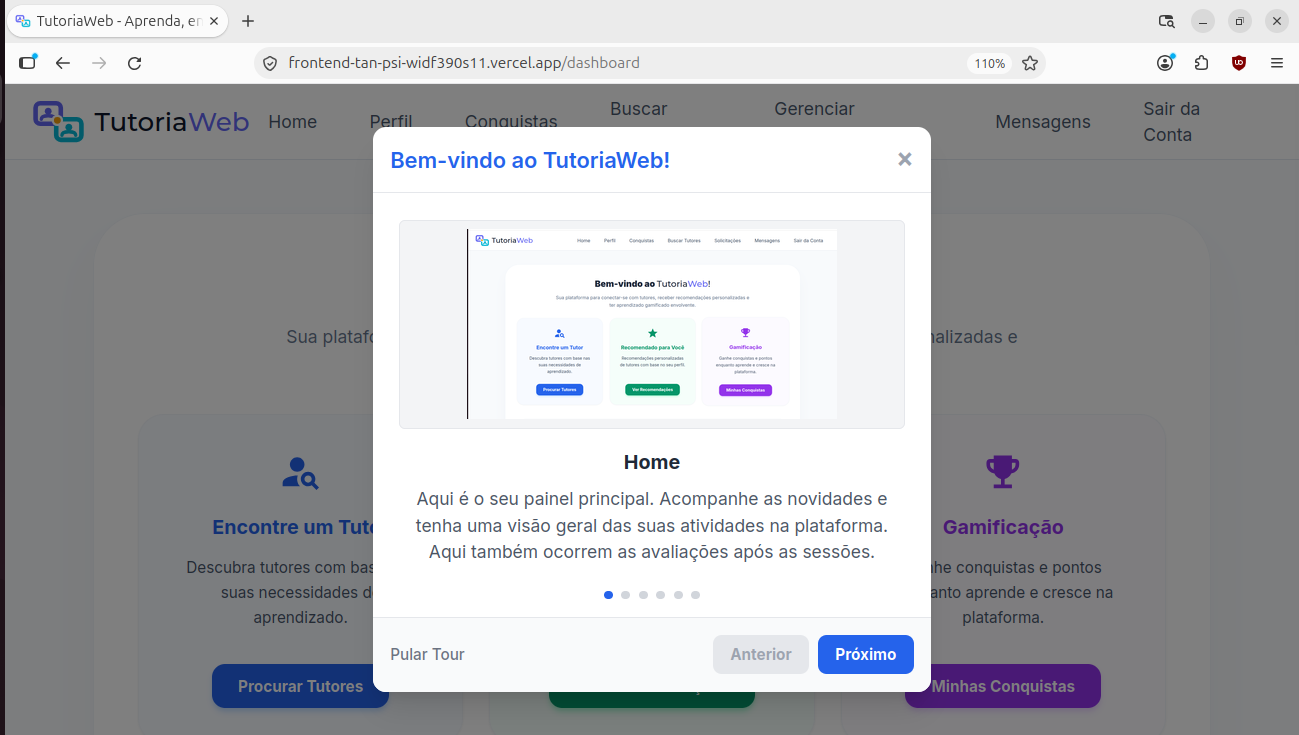
\includegraphics[width=1.9\textwidth, height=0.90\textheight, keepaspectratio]{figuras/modal-tour.png}
    
        Fonte: Autoria própria.
        
        \vspace{0.2cm}
            
        \label{fig:modal-tour}
    \end{figure}
\end{landscape}

\subsection[Análise Estática do Código]{Análise Estática do Código}

Análise estática trata-se da análise do código-fonte sem sua execução, permitindo detecção de erros de sintaxe, semântica e estrutura \cite{pressman2021engenharia}.

Para assegurar a qualidade, a segurança e a manutenibilidade do código-fonte, a aplicação SonarCloud foi adotada para realizar a análise estática contínua tanto do \textit{backend} quanto do \textit{frontend} da aplicação.

Na primeira análise, cujos resultados podem ser observados na Figura \ref{fig:analise-1}, foram identificados alguns débitos técnicos e vulnerabilidades.
Destacaram-se, neste momento inicial, a classificação "E" no quesito de segurança para o repositório do \textit{backend} e a classificação "D" em confiabilidade para o \textit{frontend}.

\begin{figure}[H]
    \centering
    \caption{Resultados da primeira análise estática.} 
    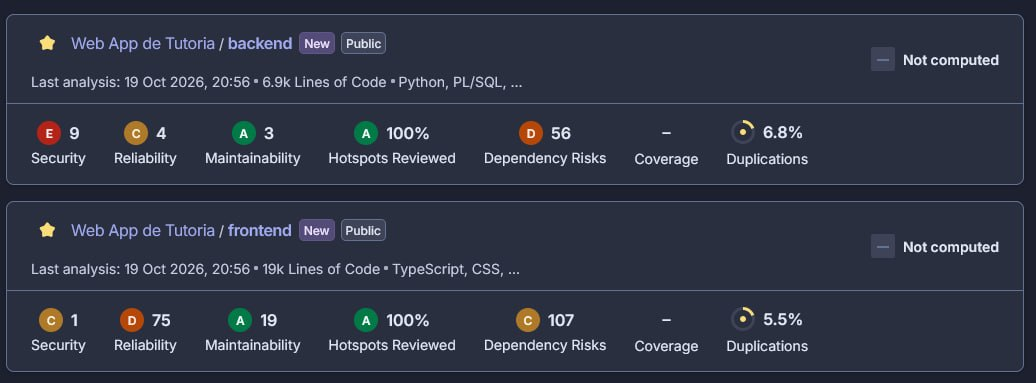
\includegraphics[width=0.99\textwidth]{figuras/analise-1.jpg}
    
    Fonte: SonarCloud.
    
    \vspace{0.2cm}
        
    \label{fig:analise-1}
\end{figure}

A partir da revisão minuciosa dos \textit{logs} e dos relatórios de apontamentos gerados pelo SonarCloud, foi feito uma refatoração dos pontos críticos indicados na base de código. Essa intervenção corretiva resultou em uma melhoria significativa no código do projeto, culminando nos indicadores exibidos na Figura \ref{fig:analise-2}.

Os erros apresentados no \textit{backend} em sua maioria eram em dependências de instalação, tanto no ``requirements.txt'' do Python quanto na inicialização do Docker com perfil \textit{root}. Além disso, também foi reportado que um dos arquivos de \textit{script} SQL (\textit{Structured Query Language}) possuia muitos comandos repetidos.

Os erros apresentados no \textit{frontend} em sua maioria eram a falta do retorno \textit{void} na chamada de funções assíncronas e o uso da tag HTML \textit{label} sem associação com campos de \textit{input} de formulários. O erro de segurança era a falta de uma configuração no arquivo Docker do \textit{frontend}, o que causava a execução de scripts antecipadamente.

Após as correções, ambos os repositórios atingiram o status de aprovação geral, zerando as vulnerabilidades de segurança e alcançando a classificação máxima ``A'' nos pilares de segurança e confiabilidade.

A classificação ``C'' em riscos de dependências no \textit{backend} se deve à versão utilizada do DRF, que era a versão estável mais recente no início do desenvolvimento. Entretanto foi verificado que para se instalar versões mais recentes, seria necessário realizar uma série de refatorações no código.

A classificação ``D'' em riscos de dependências no \textit{frontend} se deve à versão do Next.js utilizada, também a mais estável e recente na época de início do desenvolvimento. Entretanto, versões posteriores foram lançadas com otimizações e correções, sendo a falta delas os riscos apontados. Atualizar a versão do \textit{framework} poderia causar quebras de compatibilidade com bibliotecas, falhas inesperadas e comportamento inconsistente na aplicação, não sendo assim feita a atualização.


\begin{figure}[H]
    \centering
    \caption{Resultados da última análise estática.} 
    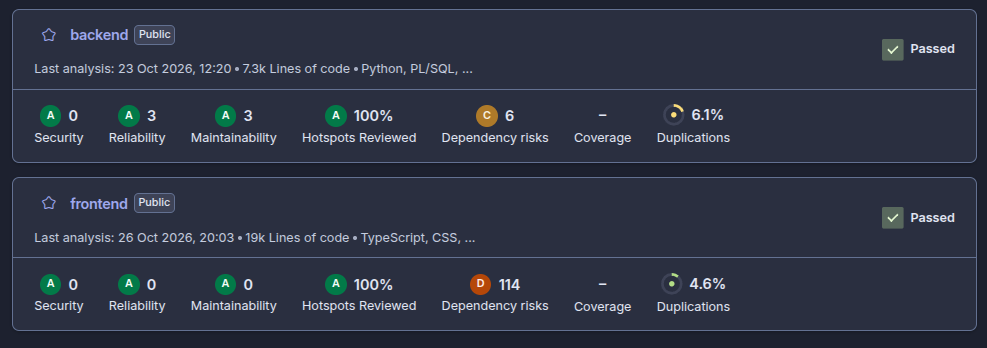
\includegraphics[width=0.99\textwidth]{figuras/analise-2.png}
    
    Fonte: SonarCloud.
    
    \vspace{0.2cm}
        
    \label{fig:analise-2}
\end{figure}